\documentclass[a4paper, 12pt, titlepage]{article}

\usepackage{amsmath}
\usepackage{amssymb}
\usepackage{bytefield}
\usepackage{fancyhdr}
\usepackage[left=2.5cm, right=2.5cm]{geometry} % for better on-line reading
\usepackage{float}
\usepackage{hyperref}
\usepackage{lastpage}
\usepackage{lettrine}
\usepackage{lmodern}
\usepackage{makecell}
\usepackage{makeidx}
\usepackage{microtype}
\usepackage{multirow}
\usepackage{setspace}
\usepackage{subcaption}
\usepackage{titlesec}
\usepackage{titling}
\usepackage[dvipsnames]{xcolor}

\usepackage[backend=biber, style=alphabetic]{biblatex}
\addbibresource{bibliography.bib}

\usepackage{listings}
\lstset{language=C++, basicstyle=\ttfamily, keywordstyle=\color{blue}\ttfamily, stringstyle=\color{red}\ttfamily}

\usepackage{pgfplots}
\pgfplotsset{compat=1.16}

\usepackage{tikz}
\usetikzlibrary{shapes,arrows,calc,fit,positioning,decorations.markings}

\renewcommand{\sectionautorefname}{}
\renewcommand{\subsectionautorefname}{}
\renewcommand{\subsubsectionautorefname}{}

% colors
\definecolor{royalblue}{cmyk}{1,0.50,0,0}
\definecolor{nemdark}{HTML}{44004E}
\definecolor{nemleading}{HTML}{5200c6}
\definecolor{nemorange}{HTML}{ff9600}
\definecolor{nemgreen}{HTML}{33dd50}

% page formatting and footer
\pagestyle{fancy}
\fancyhf{}
\cfoot{Page \thepage \hspace{1pt} of \pageref{LastPage}}

% title formatting
\titleformat{\section}
{\color{nemleading}\normalfont\Large\bfseries}
{\color{nemorange}\thesection}{1em}{}

% paragraph formatting
\setlength{\parskip}{2.5mm}
\setlength{\parindent}{4mm}

% hyperlink formatting
\hypersetup{
	colorlinks,
	linkcolor={cyan!60!black},
	citecolor={blue!50!black},
	urlcolor={blue!80!black}
}

% blue node
\tikzset{fontscale/.style = {font=\small}}
\tikzstyle{cblue}=[circle, draw, thin, fill=cyan!10, scale=0.2, align=center, fontscale=4]

% transparent node
\tikzstyle{ctra}=[rectangle, thin]
\tikzstyle{crou}=[rectangle, draw, rounded corners, thin]
\tikzstyle{crecb}=[rectangle, draw, thin, text height=12pt,text depth=5pt,solid,rounded corners=0]
\tikzstyle{legend_phytop}=[rectangle, draw, rounded corners, thin,
	minimum width=2.5cm, minimum height=0.8cm,
	royalblue
]
\tikzstyle{legend_normal}=[rectangle]

\pretitle{
	\begin{center}
	
\includegraphics{images/NEM_symbol.pdf}
	\\
	\vspace{15mm}
}

\title{
	\fontsize{26pt}{28pt}\textbf{Symbol from NEM}
	\\
	\vspace{5mm}
	\fontsize{24pt}{25pt}\textit{Technical Reference}
	\\
	\vspace{20mm}
	\fontsize{12pt}{14pt}{Version 0.10.0.4}
}
\author{}
\date{\today}

% constants
\newcommand*{\codename}{\textcolor{nemleading}{\textbf{Symbol}}}
\newcommand*{\codenamespace}{\codename{ }}
\newcommand*{\codenamechapterfirstword}{\nemchapterfirstletter{S}{ymbol} }

% math constants
\newcommand{\euler}{\mathrm{e}}

% math formatting
\newcommand{\mathfunc}[1]{\mathrm{#1}}
\newcommand{\structField}[2]{#1\mathrm{{::}#2}}

% nem index
\newcommand{\nind}[1]{
	\emph{#1}\index{#1}
}

% reference formatting
\newcommand{\nemref}[1]{\autoref{#1}:~\nameref{#1}}
\newcommand{\nemrefparens}[1]{(see \nemref{#1})}

%%% basic formatting %%%

\newcommand{\class}[1]{\texttt{#1}}
\newcommand{\field}[1]{\texttt{#1}}
\newcommand{\filepath}[1]{\texttt{#1}}

\newcommand{\nemchapterfirstletter}[1]{
	\lettrine[lraise=0,lines=3,nindent=0.5em,slope=0.0em]{\color{nemdark}\fontseries{bx}\fontsize{54pt}{56pt}\selectfont #1}
}

\protected\def \nemsetting #1#2{
	\ifmmode\text{#2}\else\textit{#1{\allowbreak}:{\allowbreak}#2}\fi
}

%%% figure formatting %%%

% centers an image without a caption
\newcommand{\nemcenter}[1]{
	\centering
	#1
}

% centers an image with a caption
\newcommand{\nemcenterwithcaption}[2]{
	\centering
	#1
	\caption{#2}
}

%%% quote formating %%%

% selects Libertine for quote font
\newcommand*\quotefont{
	\fontfamily{LinuxLibertineT-OsF}
}

\newcommand*{\openquote}{
	\tikz[remember picture,overlay,xshift=-15pt,yshift=10pt]
	\node[] (OQ) {\quotefont\fontsize{60}{60}\selectfont``};%
	\kern0pt
}
\newcommand*{\closequote}{
	\tikz[remember picture,overlay,xshift=15pt,yshift=0pt]
	\node[] (CQ) {\quotefont\fontsize{60}{60}\selectfont''};
}

\newcommand{\nemquote}[2]{
	\begin{quote}\openquote #1 \hfill\closequote
	\par \hfill \textit{- #2}
	\end{quote}
}

%%% memory layout commands %%%

% prepares an 8 byte memory layout with a caption
\newcommand{\nemmemorylayout}[2]{
	\centering
	\begin{bytefield}[bitwidth=1.1em, leftcurly=., leftcurlyspace=0pt]{8}
		\bitheader{0-7} \\
		#1
	\end{bytefield}
	\caption{#2}
}

% creates a multiword memory layout wordbox that has top-aligned text
% first param is always offset
\newcommand{\nemmemorymultiwordbox}[3]{
	\begin{leftwordgroup}{\texttt{#1}}
		\wordbox[tlr]{1}{#2}
	\end{leftwordgroup} \\
	\wordbox[blr]{#3}{}
}

% creates a multiword memory layout wordbox with variable sized data that has top-aligned text
\newcommand{\nemmemorymultiwordboxskipped}[3]{
	\begin{leftwordgroup}{\texttt{#1}}
		\wordbox[tlr]{1}{#2}
	\end{leftwordgroup} \\
	\skippedwords \\
	\wordbox[blr]{1}{#3}
}


\makeindex[intoc]

\begin{document}
	\pagenumbering{roman}

	\phantomsection\pdfbookmark[section]{\codename}{titlepage}

	\begin{titlepage}
	\maketitle
	\end{titlepage}

	\phantomsection\pdfbookmark[section]{\contentsname}{toc}

	\pagestyle{empty}
	\setcounter{page}{2}

	\begin{spacing}{0}
	{
		\pagestyle{empty}
		\fancypagestyle{plain}{
			\fancyhf{}
			\renewcommand{\headrulewidth}{0pt}
			\renewcommand{\footrulewidth}{0pt}
		}
		\tableofcontents
	}
	\end{spacing}

	\refstepcounter{section}
\section*{Preface}
\addcontentsline{toc}{section}{Preface}

\nemquote{%
You miss 100\% of the shots you don't take.
}{Wayne Gretzky}

\nemchapterfirstletter{N}{EM} had its humble beginnings as a "call for participation" on a bitcointalk thread in January 2014.
The cryptospace had just experienced a boom at the tail end of 2013 - although nowhere near where it would go a few years later - and there was a lot of enthusiasm in the space.
NXT had just launched as one of the first PoS blockchains, and much of the early NEM community was inspired by and had connections to the NXT community. This includes all three of the remaining core developers.

Although there was some initial discussion on what to build, we quickly decided to create something new from scratch.
This allowed for more design flexibility as well as the use of high coding standards from the very beginning.
This also gave us the opportunity to contribute something new to the blockchain landscape.
As a result of lots of effort - mostly nights and weekends - this culminated in the release of NIS1 mainnet in March 2015.
We were pleased with what we built, but knew we took a few shortcuts, and continued improving it.
Eventually, we came to the realization that the original solution would need a rearchitecture to fix some central performance bottlenecks and allow faster innovation in the future.

We are grateful to Tech Bureau who provided support for us to build a completely new chain from scratch - \codename.
We are hopeful that this fixes many of the problems inherent in NIS1 and provides a solid foundation for future improvements and enhancements.
Our mandate was to build a high performance *blockchain* - not a DAG or dBFT based system.
In this, we think, we succeeded.

This has been a long journey for us, but we are excited to see what yet is to come and what novel things \textbf{you} use \codenamespace to build.
We would like to once again thank the contributors and the many people who have inspired us\ldots

\begin{flushright}
	BloodyRookie
	gimre
	Jaguar0625
\end{flushright}

	\section*{Typographical conventions}
%\addcontentsline{toc}{section}{Typographical conventions}

This documentation uses the following typographical conventions:

\renewcommand{\arraystretch}{1.3}

\begin{tabular}{l p{1.5cm} p{7cm}} 
	Sample & Attributes & Description \\
	\hline
	\codenamespace & bold, colored & when referring to project name \\
	\hline
	\class{ProcessBootstrapper} & 
	\multirow[t]{3}{=}{fixed-width font} &
	\multirow[t]{3}{=}{classes, fiele paths, fields (of transactions, blocks or other entities)} \\
	\field{FeeMultiplier} & & \\
	\filepath{commit\_step.dat} & & \\
	\hline
	\nemsetting{network}{maxDifficultyBlocks} & italic & configuration settings, prefixed with configuration filename in text mode\\
	\hline
	$\nemsetting{network}{maxDifficultyBlocks}$ & regular & configuration settings, in equations and formulas \\
	\hline
	$\structField{T}{SignerPublicKey}$ & regular & model fields in equations and formulas \\
	\hline
	$\mathfunc{VerifiableDataBuffer}()$ & regular & function names in equations and formulas \\
\end{tabular}

\renewcommand{\arraystretch}{1.0}


	\setcounter{section}{0}
	\renewcommand*{\theHsection}{body\the\value{section}}

	\pagestyle{fancy}
	\pagenumbering{arabic}
	\setcounter{page}{1}

	\section{Introduction}
\label{sec:introduction}

\nemquote{%
From the ashes a fire shall be woken,\\
A light from the shadows shall spring;\\
Renewed shall be blade that was broken,\\
The crownless again shall be king.
}{J.R.R. Tolkien}

\nemchapterfirstletter{T}{rustless}, high-performance, layered-architecture, blockchain-based DLT protocol - these are the first principles that influenced the development of \codename.
While a handful of DLT protocols were considered, a blockchain protocol was quickly chosen because it was deemed most true to the ideal of trustlessness.
Any node can download a complete copy of the chain and can independently verify it at all times.
Nodes with sufficient harvesting power can always create blocks and never need to rely on a leader.
These choices necessarily sacrifice some throughput relative to other protocols, but they seem most consistent with the philosophical underpinnings of Bitcoin\cite{nakamoto2009}.

\codenamespace supports both probabilistic and deterministic block finalization.
Under probabilistic finalization, the probability that any particular block is rolled back decreases as more and more blocks are added - or chained - to it.
Although the probability might become vanishingly small, it is always nonzero\footnote{
	When probabilistic finalization is enabled, for performance reasons, at most \nemsetting{network}{maxRollbackBlocks} are allowed to be rolled back.
	Older blocks are assumed, but not guaranteed, to be finalized because the probability of their rollback is quite low.
}.
In contrast, deterministic finalization includes a mechanism in the protocol that allows checkpoints to be set that can never be rolled back.
This can lead to potentially deep rollbacks but provides stronger assurances.
In either case, the risk of block rollback and transaction invalidation is assumed by users.

As part of a focus on trustlessness, the following features were added relative to NEM:
\begin{itemize}
	\item{Block headers can be synced without transaction data, while allowing verification of chain integrity.}
	\item{Transaction Merkle trees allow cryptographic proofs of transaction containment (or not) within blocks.}
	\item{Receipts increase the transparency of indirectly triggered state changes.}
	\item{State proofs allow trustless verification of specific state within the blockchain.}
\end{itemize}

In \codename, there is a single server executable that can be customized by loading different plugins (for transaction support) and extensions (for functionality).
There are three primary configurations (per network), but further customized hybrid configurations are possible by enabling or disabling specific extensions.

The three primary configurations are:
\begin{enumerate}
	\item{Peer: These nodes are the backbone of the network and create new blocks.}
	\item{API: These nodes store data in a MongoDB database for easier querying and can be used in combination with a NodeJS REST server.}
	\item{Dual: These nodes perform the functions of both Peer and API nodes.}
\end{enumerate}

A strong network will typically have a large number of Peer nodes and enough API nodes to support incoming client requests.
Allowing the composition of nodes to vary dynamically based on real needs, should lead to a more globally resource-optimized network.

Basing the core block and transaction pipelines on the disruptor pattern - and using parallel processing wherever possible - allows high rates of transactions per second relative to a typical blockchain protocol.

NIS1 was a worthy entry into the blockchain landscape and \codenamespace is an even worthier evolution of it.
This is not the end but a new beginning.
There is more work to be done.

\subsection{Network Fingerprint}

Each network has a unique \nind{fingerprint} that is composed of the following:
\begin{enumerate}
	\item{Network Identifier -
		One byte identifier that can be shared across networks.
		All addresses compatible with a network must have this value as their first byte.
	}
	\item{Generation Hash Seed -
		Random 32 byte value that must be globally unique across networks.
		This value is prepended to transaction data prior to hashing or signing in order to prevent cross network replay attacks.
	}
\end{enumerate}

	\section{System}
\label{sec:system}

\nemquote{%
A new technology can transform society, but when the technology is in its infancy, very few people can see its full potential.
}{Liu Cixin}

\codenamechapterfirstword supports high customization at both the network and individual node levels.
Network-wide settings, specified in \nemsetting{network}{network}, must be the same for all nodes in a network.
In contrast, node-specific settings can vary across all nodes in the same network, and are located in \nemsetting{node}{node}.

\codenamespace was designed to use a \emph{plugin / extension} approach instead of supporting Turing complete smart contracts.
While the latter can allow for more user flexibility, it's also more error prone from the user perspective.
A plugin model limits the operations that can be performed on a blockchain and consequently has a smaller attack surface.
Additionally, it's much simplier to optimize the performance of a discrete set of operations than an infinite set.
This helps \codenamespace achieve the high throughput for which it was designed.

\subsection{Transaction Plugins}

All nodes in a network must support the same types of transactions and process them in exactly the same manner so that all nodes can agree on the global blockchain state.
The network requires each node to load a set of \emph{transaction plugins}\index{plugins}, and this set determines the kinds of transactions the network supports.
This set is determined by the presence of \nemsetting{network}{plugin*} sections in the \nemsetting{network}{network} configuration.
Any changes, additions or deletions of these plugins must be coordinated and accepted by all network nodes.
If only a subset of nodes agree to these modifications, those nodes will be on a fork.
All built-in \codenamespace transactions are built using this plugin model in order to validate its extensibility.

A plugin is a separate dynamically-linked library that exposes a single entry point in the following form
\footnote{Format of plugins depends on target operating system and compiler used, so all host applications and plugins must be built with the same compiler version and options.}:

\begin{lstlisting}
extern "C" PLUGIN_API
void RegisterSubsystem(
	catapult::plugins::PluginManager& manager);
\end{lstlisting}

\class{PluginManager} provides access to the subset of configuration that plugins need to initialize themselves.
Through this class, a plugin can register zero or more of the following:

\begin{enumerate}
	\item{Transactions -
		Specify new transaction types and the mapping of those types to parsing rules.
		Specifically, the plugin defines rules for translating a transaction into component notifications that are used in further processing.
		A handful of processing constraints can also be specified, such as indicating a transaction can only appear within an aggregate transaction \nemrefparens{sec:transactions:aggregate}.
	}
	\item{Caches -
		Specify new cache types and rules for serializing and deserializing model types to and from binary.
		Each state-related cache can optionally be included in the calculation of a block's \field{StateHash} \nemrefparens{sec:blocks:statehash} when that feature is enabled.
	}
	\item{Handlers - Define APIs that are always accessible.}
	\item{Diagnostics - Define APIs and counters that are accessible only when the node is running in diagnostic mode.}
	\item{Validators - Process the notifications produced by block and transaction processing.
			These validators can be stateless or stateful.
			The registered validators can subscribe to general or plugin-defined notifications and reject disallowed values or state changes.
	}
	\item{Observers - Process the notifications produced by block and transaction processing.
		The registered observers can subscribe to general or plugin-defined notifications and update blockchain state based on their values.
		Observers don't require any validation logic because they are only called after all applicable validators succeed.
	}
	\item{Resolvers -
		Specify custom mappings from unresolved to resolved types.
		For example, this is used by the namespace plugin to add support for alias resolutions
\nemrefparens{sec:accounts:addressaliases}.
	}
\end{enumerate}

\subsection{\codenamespace Extensions}
\label{sec:system:extensions}

Individual nodes within a network are allowed to support a heterogeneous mix of capabilities.
For example, some nodes might want to store data in a database or publish events to a message queue.
These capabilities are all optional because none of them impact consensus.
Such capabilities are determined by the set of \nind{extensions} a node loads as specified in \nemsetting{extensions-\{process\}}{extensions}.
Most built-in \codenamespace functionality is built using this extension model in order to validate its extensibility.

An extension is a separate dynamically linked library that exposes a single entry point in the following form
\footnote{Format of extensions depends on target operating system and compiler used, so all host applications and plugins must be built with the same compiler version and options.}:

\begin{lstlisting}
extern "C" PLUGIN_API
void RegisterExtension(
	catapult::extensions::ProcessBootstrapper& bootstrapper);
\end{lstlisting}

\class{ProcessBootstrapper} provides access to full \codenamespace configuration and services that extensions need to initialize themselves.
Providing this additional access allows extensions to be more powerful than plugins.
Through this class, an extension can register zero or more of the following:

\begin{enumerate}
	\item{Services -
		Represent an independent behavior.
		Services are passed an object representing the executable's state and can use it to configure a multitude of things.
		Among others, a service can add diagnostic counters, define APIs (both diagnostic and non-diagnostic) and add tasks to the task scheduler.
		It can also create dependent services and tie their lifetimes to that of the hosting executable.
		There are very few limitations on what a service can do, which allows the potential for significant customizations.
	}
	\item{Subscriptions -
		Process any supported blockchain event: block, state, unconfirmed transaction and partial transaction.
		Events are raised when changes are detected.
		Transaction status events are raised when the processing of a transaction completes.
		Node events are raised when remote nodes are discovered.
	}
\end{enumerate}

In addition to the above, extensions can configure the node in more intricate ways.
For example, an extension can register a custom network time supplier.
In fact, there is a specialized extension that sets a time supplier based on algorithms described in \nemref{sec:timesync}.
This is an example of the high levels of customization allowed by this extension model.
For understanding the full range of extensibility allowed by extensions, please refer to the project code or developer documentation\nemtechdocsfootnote{}.

\subsection{Server}

The simplest \codenamespace topology is composed of a single server executable.
Transaction Plugins required by the network and \codenamespace Extensions desired by the node operator are loaded and initialized by the server.

\codenamespace stores all of its data in a \filepath{data} directory.
The contents of the data directory are as follows:

\begin{enumerate}
	\item{Block Versioned Directories -
		These directories contain block information in a proprietary format.
		Each confirmed block's binary data, transactions and associated data are stored in these directories.
		The statements \nemrefparens{sec:blocks:receipts} generated when processing each block are also stored here for quick access.
		An example of a versioned directory is \filepath{00000}, which contains the first group of blocks.
	}
	\item{\filepath{audit} - Audit files created by the audit consumer \nemrefparens{sec:disruptor:commonConsumers} are stored in this directory.}
	\item{\filepath{spool} -
		Subscription notifications are written out to this directory.
		They are used as a message queue to pass messages from the server to the broker.
		They are also used by the recovery process to recover data in the case of an ungraceful termination.
	}
	\item{\filepath{state} -
		\codenamespace stores its proprietary storage files in this directory.
		\filepath{supplemental.dat} and files ending with \filepath{\_summary.dat} store summarized data.
		Files ending in \filepath{Cache.dat} store complete cache data.
	}
	\item{\filepath{statedb} - When \nemsetting{node}{enableCacheDatabaseStorage} is set, this directory will contain RocksDB files.}
	\item{\filepath{transfer\_message} -
		When \nemsetting{user}{enableDelegatedHarvestersAutoDetection} is set, this directory will contain extracted delegated harvesting requests for the current node.
	}
	\item{\filepath{commit\_step.dat} -
		This stores the most recent step of the commit process initiated by the server.
		This is primarily used for recovery purposes.
	}
	\item{\filepath{index.dat} - This is a counter that contains the number of blocks stored on disk.}
\end{enumerate}

\subsubsection{Cache Database}

The server can run with or without a cache database.
When \nemsetting{node}{enableCacheDatabaseStorage} is set, RocksDB is used to store cache data.
Verifiable state \nemrefparens{sec:blocks:statehash} requires a cache database and most network configurations are expected to have it enabled.

A cache database should only be \emph{disabled} when all of the following are true:

\begin{enumerate}
	\item{High rate of transactions per second is desired.}
	\item{Trustless verification of cache state is not important.}
	\item{Servers are configured with a large amount of RAM.}
\end{enumerate}

In this mode, all cache entries are always resident in memory.
On shutdown, cache data is written to disk across multiple flat files.
On startup, this data is read and used to populate the memory caches.

When a cache database is enabled, summarized cache data is written to disk across multiple flat files.
This summarized data is derivable from data stored in caches.
One example is the list all high-value accounts that have a balance of at least \nemsetting{network}{minHarvesterBalance}.
While this list can be generated by (re)inspecting all accounts stored in the account state cache, it is saved to and loaded from disk as an optimization.

\subsection{Broker}

The broker process allows more complex \codenamespace behaviors to be added without sacrificing parallelization.
Transaction Plugins required by the network and \codenamespace Extensions desired by the node operator are loaded and initialized by the broker.
Although the broker supports all features of Transaction Plugins, it only supports a subset of \codenamespace Extensions features.
For example, overriding the network time supplier in the broker is not supported.
Broker extensions are primarily intended to register subscribers and react to events forwarded to those subscribers.
Accordingly, it's expected that the server and broker have different extensions loaded.
Please refer to the project code or developer documentation for more details.

The broker monitors the \filepath{spool} directories for changes and forwards any event notifications to subscribers registered by loaded extensions.
Extensions register their subscribers to process these events.
For example, a database extension can read these events and use them to update a database to accurately reflect the global blockchain state.

\filepath{spool} directories function as one way message queues.
The server writes messages and the broker reads them.
There is no way for the broker to send messages to the server.
This decoupling is intentional and was done for performance reasons.

The server raises subscription events in the blockchain sync consumer \nemrefparens{sec:disruptor:blockConsumers} when it holds an exclusive lock to the blockchain data.
These operations are offloaded to the broker to prevent slow database operations when the server has an exclusive lock.
The server overhead is minimal because most of the data used by the broker is also required to recover data after an ungraceful server termination.

\subsection{Recovery}

The recovery process is used to repair the global blockchain state after an ungraceful server and/or broker termination.
Transaction Plugins required by the network and \codenamespace Extensions desired by the node operator are loaded and initialized by the recovery process.
When a broker is used, the recovery process must load the same extensions as the broker.

The specific recovery procedure depends on the process configuration and the value of the \filepath{commit\_step.dat} file.
Generally, if the server exited after state changes were flushed to disk, those changes will be reapplied.
The blockchain state will be the same as if the server had applied and committed those changes.
Otherwise, if the server exited before state changes were flushed to disk, pending changes will be discarded.
The blockchain state will be the same as if the server had never attempted to process those changes.

After the recovery process completes, the blockchain state should be indistinguishable from the state of a node that never terminated ungracefully.
\filepath{spool} directories are repaired and processed.
Block and cache data stored on disk are reconciled and updated.
Pending state changes, if applicable, are applied.
Other files indicating the presence of an ungraceful termination are updated or removed.

\subsection{Common Topologies}

Although a network can be composed of a large number of heterogeneous topologies, it is likely that most nodes will fall into one of three categories: Peer, API or Dual.
The same server process is used across all of these topologies.
The only difference is in what extensions each loads.

Peer nodes are lightweight nodes.
They have enough functionality to add security to the blockchain network, but little beyond that.
They can synchronize with other nodes and harvest new blocks.

API nodes are more heavyweight nodes.
They can synchronize with other nodes, but cannot harvest new blocks.
They support hosting bonded aggregate transactions and collecting cosignatures to complete them.
They require a broker process, which is configured to write data into a MongoDB database and propagate changes over public message queues to subscribers.
The REST API is dependent on both of these capabilities and is typically co-located with an API node for performance reasons in order to minimize latency.

Dual nodes are simply a superset of Peer and API nodes.
They support all capabilities of both node types.
Since these nodes support all API node capabilities, they also require a broker.

	\section{Cryptography}
\label{sec:cryptography}

\nemquote{%
I understood the importance in principle of public key cryptography but it's all moved much faster than I expected. I did not expect it to be a mainstay of advanced communications technology.
}{Whitfield Diffie}

\nemchapterfirstletter{B}{lockchain} technology demands the use of some cryptographic concepts.
\codenamespace uses cryptography based on Elliptic Curve Cryptography (ECC).
The choice of the underlying curve is important in order to guarantee security and speed.

\codenamespace uses the Ed25519\index{Ed25519} digital signature algorithm.
This algorithm uses the following \emph{Twisted Edwards curve}:
$$ -x^2 + y^2 = 1 - \frac{121665}{121666} x^2 y^2$$
over the finite field defined by the prime number $2^{255}-19$.
The base point for the corresponding group G is called B.
The group has $q=2^{252} + 27742317777372353535851937790883648493$ elements.
It was developed by D. J. Bernstein et al. and is one of the safest and fastest digital signature algorithms \cite{Bernstein2011}.

Importantly for \codenamespace purposes, the algorithm produces short 64-byte signatures and supports fast signature verification.
Neither key generation nor signing is used during block processing, so the speed of these operations is unimportant.

\subsection{Public/Private Key Pair}
\index{key!private}
\index{key!public}

A \emph{private key} is a random 256-bit integer $k$. To derive the public key\emph{public key} \underline{A} from it, the following steps are taken:
\begin{align}
	\hf(k) &=(h_0, h_1, \ldots, h_{511}) \\
	a &= 2^{254} + \sum_{3\leq i \leq 253} 2^i h_i \\
	A &= aB
\end{align}

Since $A$ is a group element, it can be encoded into a 256-bit integer \underline{A}, which serves as the public key.

\subsection{Signing and Verification}

Given a message $M$, private key $k$ and its associated public key \underline{A}, the following steps are taken to create a signature:
\begin{align}
	\hf(k) &=(h_0, h_1, \ldots, h_{511}) \\
	r &= \hf(h_{256}, \ldots, h_{511}, M) \text{ where the comma means concatenation} \\
	R &= rB \\
	S &= (r + \hf(\underline{R}, \underline{A}, M)a) \: mod \: q \label{eq:cryptography:S}
\end{align}

Then $(\underline{R}, \underline{S})$ is the \nind{signature} for the message $M$ under the private key $k$.
Note that only signatures where $S<q$ and $S>0$ are considered as valid \textbf{to prevent} the problem of \emph{signature malleability}\index{signature!malleability}.

To verify the signature $(\underline{R}, \underline{S})$ for the given message $M$ and public key \underline{A}, the verifier checks $S<q$ and $S>0$ and then calculates
\begin{align*}
	\tilde{R} = SB - \hf(\underline{R}, \underline{A}, M)A
\end{align*}

and verifies that
\begin{equation}
	\tilde{R} = R \label{eq:cryptography:verifyR}
\end{equation}

If $S$ was computed as shown in \eqref{eq:cryptography:S} then
$$SB = rB + (\hf(\underline{R}, \underline{A}, M)a)B = R + \hf(\underline{R}, \underline{A}, M)A$$
so \eqref{eq:cryptography:verifyR} will hold.

\subsubsection{Batch Verification}

When lots of signatures have to be verified, a batch signature verification can speed up the process by about 80\%.
\codenamespace uses the algorithm outlined in \cite{Bernstein2011}.
Given a batch of $(M_i, A_i, R_i, S_i)$ where $(R_i, S_i)$ is the signature for the message $M_i$ with public key $A_i$,
let $H_i = \hf(R_i, A_i, M_i)$.
Additionally, assume a corresponding number of uniform distributed 128-bit independent random integers $z_i$ are generated.
Now consider the equation:
\begin{align}
	\left(-\sum_i{z_i S_i \: \mathrm{mod} \: q}\right)B + \sum_i{z_i R_i} + \sum_i{(z_i H_i \: \mathrm{mod} \: q)A_i = 0} \label{eq:cryptography:verifyBatch}
\end{align}

Setting $P_i = 8 R_i + 8 H_i A_i - 8 S_i B$, then if \eqref{eq:cryptography:verifyBatch} holds, it implies
\begin{align}
	\sum_i{z_i P_i} = 0 \label{eq:cryptography:verifyBatch2}
\end{align}

All $P_i$ are elements of a cyclic group (remember $q$ is a prime).
If some $P_i$ is not zero, for example $P_2$, it means that for given integers $z_0, z_1, z_3, z_4 \ldots$, there is exactly one choice for $z_2$ to satisfy \eqref{eq:cryptography:verifyBatch2}.
The chance for that is $2^{-128}$.
Therefore, if \eqref{eq:cryptography:verifyBatch} holds, it is a near certainty that $P_i = 0$ for all $i$.
This implies that the signatures are valid.

If \eqref{eq:cryptography:verifyBatch} does not hold, it means that there is at least one invalid signature.
In that case, \codenamespace falls back to single signature verification to identify the invalid signatures.

\subsection{Verifiable Random Function (VRF)}
\label{sec:cryptography:vrf}

A verifiable random function (\nind{VRF}) uses a public/private key pair to generate pseudo-random values.
Only the owner of the private key can generate a value such that it cannot be predetermined by an adversary.
Anyone with the public key can verify whether or not the value was generated by its associated private key.
\codenamespace uses the ECVRF-EDWARDS25519-SHA512-TAI defined in \cite{irtf-cfrg-vrf-07}.

To generate a proof\footnote{
	This is typically called proving, not to be confused with verifying, because the private key owner needs to prove that it generated
	the random value with its private key.
} given a public key $Y$ corresponding to a private key $SK = xB$ and an input seed $alpha$\footnote{
	The listings provided in this section do not define auxiliary functions.
	Full descriptions of these functions can be found in \cite{irtf-cfrg-vrf-07}.
}:
\begin{align*}
	H &= \mathfunc{map\_to\_group\_element}(alpha, Y) \\
	\gamma &= xH \\
	k &= \mathfunc{generate\_nonce}(H) \\
	c &= \mathfunc{IetfHash}(3, 2, H, \gamma, kB, kH)[0..15] \\
	s &= (k + cx) \mod q \\
	proof &= (\gamma, c, s)
\end{align*}

The proof produced by the function above can be verified with the following procedure:
\begin{align*}
	H &= \mathfunc{map\_to\_group\_element}(alpha, Y) \\
	U &= sB - cY \\
	V &= sH - c \gamma \\
	\mathvar{verification\_hash} &= \mathfunc{IetfHash}(3, 2, H, \gamma, U, V)[0..15]
\end{align*}

When the calculated $\mathvar{verification\_hash}$ matches the $c$ part of the proof, the verification of the random value is successful.

A proof hash, also called a VRF hash output, can be derived from $\gamma$ of a \emph{validated} proof:
\begin{align}
	\mathvar{proof\_hash} &= \mathfunc{IetfHash}(3, 3, 8 \gamma) \label{eq:cryptography:proofHash}
\end{align}

\subsection{Voting Key Tree}
\label{sec:cryptography:voting}
\index{tree!BM (Bellare-Miner)}
\index{BM tree|see {tree, BM (Bellare-Miner)}}

Finalization voters are required to specify the range of epochs in which a root voting key is eligible to vote.
Prior to announcing a root voting key, voters are required to build a voting key tree that contains epoch-pinned voting keys.
The tree construction is roughly based on Bellare-Miner \cite{BellareMiner1999} construction.

A two-level tree is used in the current implementation.
The amount of keys in the lowest level is dependent on the \nemsetting{finalization}{votingKeyDilution} setting\footnote{
	This setting must be the same across all network nodes.
}.

\newcommand{\key}[1]{ node { $sk_{#1}$ \\ $pk_{#1}$ \\ $sig_{#1}$ } }
\begin{figure}[h]
	\nemcenterwithcaption{
		\begin{tikzpicture}[font=\small,every node/.style = {shape=rectangle, rounded corners, draw, align=center}]]
		\tikzset{
			used/.style = { text=gray!30 },
			unused/.style = { text=black },
		}
		\tikzstyle{level 1}=[level distance=10em]
		\tikzstyle{level 2}=[level distance=6em]
		\node { root voting public key }
			child [used, sibling distance=15em] { \key{b_1}
				child [sibling distance=4em] { \key{b_{1,0}} }
				child [sibling distance=4em] { \key{b_{1,1}} }
				child [unused, sibling distance=1.5em] { node[draw=none] { \ldots } }
				child [sibling distance=3em] { \key{b_{1,d-1}} }
			}
			child [used, sibling distance=15em] { \key{b_2}
				child [used, sibling distance=4em] { \key{b_{2,0}} }
				child [unused, sibling distance=4em] { \key{b_{2,1}} }
				child [unused, sibling distance=1.5em] { node[draw=none] { \ldots } }
				child [unused, sibling distance=3em] { \key{b_{2,d-1}} }
			}
			child [sibling distance=2em] { node[draw=none] { \vdots } }
			child [sibling distance=3em] { \key{b_n}
				child [used] { node { sub-tree \\ not ready } }
			};
		\end{tikzpicture}
	}{Voting key tree with $d := \nemsetting{finalization}{votingKeyDilution}$ }
\end{figure}

The tree is built by pinning keys to identifiers in the tree. The identifiers in the tree are derived from the epoch.
\begin{align}
	i &= \mathfunc{floor}(\mathvar{epoch} / \nemsetting{finalization}{votingKeyDilution}) \\
	j &= \mathvar{epoch} \bmod \nemsetting{finalization}{votingKeyDilution}
\end{align}

$i$ is an index into the middle layer of the tree relative to the root.
$j$ is an index into the bottom layer of the tree relative to the middle layer.
$b_i$ is an index from the root to the \emph{i} middle layer.
$b_{i,j}$ is an index from the root to the \emph{i} middle layer and from there to the \emph{j} bottom layer.

The tree is partially built before announcing a voting key link transaction.
First, the \emph{tree root key pair} is generated.
The root public key is signed with an account's signing public key as part of the voting key link transaction.

Next, middle-level keys are generated and, for each key pair, the public key is signed with the root key.
After all middle-level keys are generated, the \emph{root secret key} is discarded.
\begin{align*}
	\mathvar{sig}_{b_i} &= \mathfunc{Sign}_{\mathname{root secret key}}(\mathvar{pk}_{b_i} || \mathfunc{IntToBin}(i))
\end{align*}

When requested, a batch of \nemsetting{finalization}{votingKeyDilution} bottom-level keys are generated in a similar fashion.
When the batch is generated, the middle-level secret key is discarded.
\begin{align*}
	\mathvar{sig}_{b_{i,j}} &= \mathfunc{Sign}_{\mathvar{sk}_{b_i}}(\mathvar{\mathvar{pk}_{b_{i, j}} || \mathfunc{IntToBin}(j) })
\end{align*}

\index{key!BM tree signing}

Therefore, every \emph{BM tree signing key} is composed of three parts:
\begin{itemize}
	\item{top-level: $\mathname{root voting public key}$}
	\item{middle-level: $(\mathvar{pk}_{b_i}, \mathvar{sig}_{b_i})$}
	\item{bottom-level: $(\mathvar{sk}_{b_i, j}, \mathvar{pk}_{b_i, j}, \mathvar{sig}_{b_i})$}
\end{itemize}

A bottom-level key is only valid for a single epoch, and then it is discarded.
When in use, all the higher level keys that have generated the bottom level key have already been destroyed.
Using a unique short-term key for each epoch prevents long range attacks revolving around an attacker collecting old and discarded finalization keys.

When signing a voting message for a given epoch, a bottom-level signature is created:
\begin{align*}
	\mathvar{sig}_{\mathname{message-i,j}} &= \mathfunc{Sign}_{\mathvar{sk}_{b_{i,j}}}(message)
\end{align*}

\index{signature!BM tree}

Finally, the signature for a vote in a given epoch - called \emph{BM tree signature} - is composed of three pairs:
\begin{itemize}
	\item{$(\mathname{root voting public key}, \mathvar{sig}_{b_i} )$}
	\item{$(\mathvar{pk}_{b_i}, \mathvar{sig}_{b_{i, j}})$}
	\item{$(\mathvar{pk}_{b_{i,j}}, \mathvar{sig}_{\mathname{message-i,j}})$}
\end{itemize}

A \emph{BM tree signature} is considered verified when:
\begin{itemize}
	\item{\emph{root voting public key} is registered to participate in the given epoch.}
	\item{\emph{middle-level} and \emph{bottom-level} keys match epoch.}
	\item{All component signatures are cryptographically verified.}
\end{itemize}

	\section{Trees}
\label{sec:trees}

% custom tree commands
\newcommand{\nemtree}[2]{
	\nemcenterwithcaption{
		\begin{tikzpicture}[every node/.style = {shape=rectangle, rounded corners, draw, align=center}]]
			#1
		\end{tikzpicture}
	}{#2}
}

\newcommand{\nemtreelabeled}[3]{
	\nemtree{#1}{#2\label{fig:trees:#3}}
}

\nemquote{%
All our wisdom is stored in the trees.
}{Santosh Kalwar}

\codenamechapterfirstword uses tree structures in order to support trustless light clients.
Merkle trees allow a client to cryptographically confirm the existence of data stored within them.
Patricia trees allow a client to cryptographically confirm the existence or non-existence of data stored within them.

\subsection{Merkle Tree}

A Merkle Tree\cite{Merkle1988} is a tree of hashes that allows efficient existence proofs.
Within \codename, all basic merkle trees are constrained to being balanced and binary.
Each leaf node contains a hash of some data.
Each non-leaf node is constructed by hashing the hashes stored in child nodes.
In the \codenamespace implementation, when any (non-root) layer contains an odd number of hashes, the last hash is doubled when calculating the parent hash.

\begin{figure}[h]
	\nemtree{
		\tikzstyle{level 3}=[sibling distance=8em]
		\node {Merkle Hash = $H_{Root}$ =\\ $\hf(H_{ABCD}, H_{EE^2})$}
			child [sibling distance=16em] { node {$H_{ABCD}$ =\\ $\hf(H_{AB}, H_{CD})$}
				child { node {$H_{AB}$ =\\ $\hf(\hf(A), \hf(B))$}
					child { node { $\hf(A)$ } { child { node {A} } } }
					child { node { $\hf(B)$ } { child { node {B} } } }
				}
				child { node {$H_{CD}$ =\\ $\hf(\hf(C), \hf(D))$ }
					child { node { $\hf(C)$ } { child { node {C} } } }
					child { node { $\hf(D)$ } { child { node {D} } } }
				}
			}
			child [sibling distance=16em] { node {$H_{EE^2}$ =\\ $\hf(H_{EE}, H_{EE})$}
				child { node {$H_{EE}$ =\\ $\hf(\hf(E), \hf(E))$ }
					child { node { $\hf(E)$ } { child { node {E} } } }
				}
			};
	}{Four level Merkle tree composed of five data items}
\end{figure}

\begin{figure}
	\nemtree{
		\tikzset{ highlight/.style = {fill = yellow} }
		\tikzstyle{level 3}=[sibling distance=8em]
		\node [highlight] {Merkle Hash = $H_{Root}$ =\\ $\hf(H_{ABCD}, H_{EE^2})$}
			child [sibling distance=16em] { node {$H_{ABCD}$ =\\ $\hf(H_{AB}, H_{CD})$}
				child { node {$H_{AB}$ =\\ $\hf(\hf(A), \hf(B))$ }
					child { node [highlight] { $\hf(A)$ } { child { node {A} } } }
					child { node { $\hf(B)$ } { child { node [highlight] {B} } } }
				}
				child { node [highlight] {$H_{CD}$ =\\ $\hf(\hf(C), \hf(D))$ }
					child { node { $\hf(C)$ } { child { node {C} } } }
					child { node { $\hf(D)$ } { child { node {D} } } }
				}
			}
			child [sibling distance=16em] { node [highlight] {$H_{EE^2}$ =\\ $\hf(H_{EE}, H_{EE})$}
				child { node {$H_{EE}$ =\\ $\hf(\hf(E), \hf(E))$ }
					child { node { $\hf(E)$ } { child { node {E} } } }
				}
			};
	}{Merkle proof required for proving existence of B in the tree}
\end{figure}

A benefit of using merkle trees is that the existence of a hash in a tree can be proven with only $\log(N)$ hashes.
This allows for existence proofs with relatively low bandwidth requirements.

A merkle proof for existence requires a single hash from each level of the tree.
In order to prove the existence of $B$, a client must:
\begin{enumerate}
	\item{Calculate $\hf(B)$.}
	\item{Obtain $H_{Root}$; in \codename, this is stored in the block header.}
	\item{Request $\hf(A), H_{CD}, H_{EE^2}$.}
	\item{Calculate $H_{Root'} = \hf(\hf(\hf(\hf(A), \hf(B)), H_{CD}), H_{EE^2})$.}
	\item{Compare $H_{Root}$ and $H_{Root'}$; if they match $\hf(B)$ must be stored in the tree.}
\end{enumerate}

\subsection{Patricia Tree}
\label{sec:trees:patricia}

A patricia tree\cite{Morrison1968} is a deterministically ordered tree.
It is constructed from key value pairs, and supports both existence and non-existence proofs requiring only $\log(N)$ hashes.
Non-existence proofs are possible because this tree is deterministically sorted by keys.
The application of the same data, in any order, will always result in the same tree.

When inserting a new key value pair into the tree, the key is decomposed into nibbles and each nibble is logically its own node in the tree.
All keys within a single tree are required to have the same length, which allows slightly optimized algorithms.

For illustration, consider the following key value pairs in \autoref{tab:trees:exampleData}.
Some examples will use ASCII keys to more clearly elucidate concepts, while others will use hex keys to more accurately depict \codenamespace implementations.

\autoref{fig:trees:asciiExpanded} depicts a full patricia tree where each letter is represented by a separate node.
Although this tree is logically correct, it is quite expansive and uses a lot of memory.
A typical key is a 32 byte hash value, which implies that storing a single value could require up to 64 nodes.
In order to work around this limitation, successive empty branch nodes can be collapsed into either a branch node with at least two connections or a leaf node.
This leads to a different but more compact tree, as depicted in \autoref{fig:trees:asciiCompact}.

\begin{table}[ht]
	\nemcenterwithcaption{
		\begin{tabular}{|c|c|c|}
			\hline
			key & hex-key & value \\
			\hline
			do** & \texttt{646F0000} & verb \\
			dog* & \texttt{646F6700} & puppy \\
			doge & \texttt{646F6765} & mascot \\
			hors & \texttt{686F7273} & stallion \\
			\hline
		\end{tabular}
	}{Patricia tree example data\label{tab:trees:exampleData}}
\end{table}

\begin{figure}[H]
	\nemtreelabeled{
		\tikzstyle{level 1}=[sibling distance=20em]
		\tikzstyle{level 3}=[sibling distance=16em]
		\tikzstyle{level 4}=[sibling distance=8em]
		\node {Root}
			child { node {D}
				child { node {O}
					child { node {*}
						child { node {* [verb]} }
					}
					child { node {G}
						child { node {* [puppy]} }
						child { node {E [mascot]} }
					}
				}
			}
			child { node {H}
				child { node {O}
					child { node {R}
						child { node {S [stallion]} }
					}
				}
			};
	}{Conceptual (expanded) patricia tree composed of four data items
	}{asciiExpanded}
\end{figure}

\begin{figure}[H]
	\nemtreelabeled{
		\tikzset{ highlight/.style = {fill = yellow} }
		\tikzstyle{level 1}=[sibling distance=20em]
		\tikzstyle{level 3}=[sibling distance=16em]
		\tikzstyle{level 4}=[sibling distance=8em]
		\node {Root}
			child { node [highlight] {DO}
				child { node [highlight] {** [verb]} }
				child { node {G}
					child { node {* [puppy]} }
					child { node {E [mascot]} }
				}
			}
			child { node [highlight] {HORS [stallion]} };
	}{Conceptual (compact) patricia tree composed of four data items
	}{asciiCompact}
\end{figure}

\subsection{Merkle Patricia Tree}

A merkle patricia tree is a combination of merkle and patricia trees.
The \codenamespace implementation centers around two types of nodes: leaf nodes and branch nodes.
Each leaf node contains a hash of some data.
Each branch node contains up to sixteen pointers to child nodes.

Like in a basic merkle tree, each merkle patricia tree has a root hash.
Unlike in a basic merkle tree, the hashes stored in the tree are a bit more complex.

Every node in the tree has a tree node path.
This path is composed of a sentinel nibble followed by zero or more path nibbles.
If the path represents a leaf node, $\texttt{0x2}$ will be set in the sentinel nibble.
If the path is composed of an odd number of nibbles, $\texttt{0x1}$ will be set in the sentinel nibble and the second nibble will contain the first path nibble.
If the path is composed of an even number, the second nibble will be set to $\texttt{0x0}$ and the second byte will contain the first path nibble.

\begin{figure}[ht]
	\nemcenterwithcaption{
		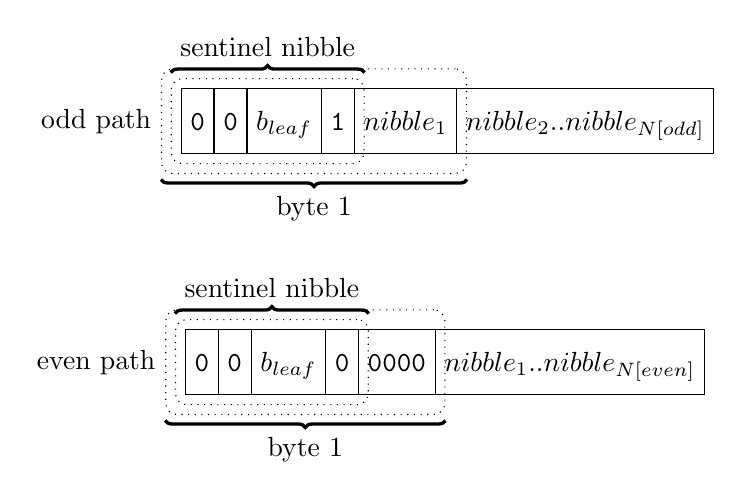
\begin{tikzpicture}[node distance=-\pgflinewidth]
			% odd tree node path
			\node[anchor=center] (lbl1) {odd path};
			\node[crecb,right=0.25cm of lbl1] (bit11) {\texttt{0}};
			\node[crecb,right=of bit11] (bit12) {\texttt{0}};
			\node[crecb,right=of bit12] (bit13) {$b_{leaf}$};
			\node[crecb,right=of bit13] (bit14) {\texttt{1}};

			\node[crecb,right=of bit14] (nibble12) {$nibble_1$};
			\node[crecb,right=of nibble12] {$nibble_2..nibble_{N [odd]}$};

			\node[fit=(bit11)(bit12)(bit13)(bit14), draw, dotted, rounded corners] (nibble11) {};
			\draw[decorate,decoration={brace,raise=2pt},very thick] (nibble11.north west) -- node[above=4pt] {sentinel nibble} (nibble11.north east);

			\node[fit=(nibble11)(nibble12), draw, dotted, rounded corners] (byte11) {};
			\draw[decorate,decoration={brace,mirror,raise=2pt},very thick] (byte11.south west) -- node[below=4pt] {byte 1} (byte11.south east);

			% even tree node path
			\node[anchor=center, below=2.5cm of lbl1] (lbl2) {even path};
			\node[crecb,right=0.25cm of lbl2] (bit21) {\texttt{0}};
			\node[crecb,right=of bit21] (bit22) {\texttt{0}};
			\node[crecb,right=of bit22] (bit23) {$b_{leaf}$};
			\node[crecb,right=of bit23] (bit24) {\texttt{0}};

			\node[crecb,right=of bit24] (nibble22) {\texttt{0000}};
			\node[crecb,right=of nibble22] {$nibble_1..nibble_{N [even]}$};

			\node[fit=(bit21)(bit22)(bit23)(bit24), draw, dotted, rounded corners] (nibble21) {};
			\draw[decorate,decoration={brace,raise=2pt},very thick] (nibble21.north west) -- node[above=4pt] {sentinel nibble} (nibble21.north east);

			\node[fit=(nibble21)(nibble22), draw, dotted, rounded corners] (byte21) {};
			\draw[decorate,decoration={brace,mirror,raise=2pt},very thick] (byte21.south west) -- node[below=4pt] {byte 1} (byte21.south east);
		\end{tikzpicture}
	}{Tree node path encoding}
\end{figure}

A \emph{leaf node}\index{tree!leaf} is composed of the following two items:
\begin{enumerate}
	\item{TreeNodePath: Encoded tree node path (with leaf bit set).}
	\item{ValueHash: Hash of the value associated with the key ending at the leaf.}
\end{enumerate}

The hash of a leaf node can be calculated by hashing its component parts:
$$\hf(\mathvar{Leaf}) = \hf(\mathvar{TreeNodePath}, \mathvar{ValueHash})$$.

A \emph{branch node}\index{tree!branch} is composed of the following items:
\begin{enumerate}
	\item{TreeNodePath: Encoded tree node path (with leaf bit unset).}
	\item{
		$\mathvar{LinkHash}_{0}, \ldots, \mathvar{LinkHash}_{15}$: Hashes of children where the index is the next nibble part of the path.
		When no child is present at an index, a zero hash should be used instead.
	}
\end{enumerate}

The hash of a branch node can be calculated by hashing its component parts:
$$\hf(\mathvar{Branch}) = \hf(\mathvar{TreeNodePath}, \mathvar{LinkHash}_0,\ldots,\mathvar{LinkHash}_{15})$$.

Reconstructing the earlier example with hex keys yields a tree that illustrates a more accurate view of how a \codenamespace tree is constructed.
Notice that each branch node index composes a single nibble of the path.
This is depicted in \autoref{fig:trees:hexCompact}.

\begin{figure}[ht]
	\nemtreelabeled{
		\tikzstyle{level 1}=[sibling distance=20em]
		\tikzstyle{level 3}=[sibling distance=16em]
		\tikzstyle{level 4}=[sibling distance=8em]
		\node (6) [red] {\texttt{6}}
			child { node (646F) [red] {\texttt{6F}}
				child { node (646F0000) {\texttt{000} [verb]} }
				child { node (646F67) [red] {\texttt{7}}
					child { node (646F6700) {\texttt{0} [puppy]} }
					child { node (646F6765) [red] {\texttt{5} [mascot]} }
				}
			}
			child { node (686F7273) {\texttt{6F7273} [stallion] } };

		\begin{scope}[every node/.style = {draw=none}]
			\path (6) -- (646F) node [red, above, pos=0.5] {{\texttt{4}}};
			\path (6) -- (686F7273) node [above, pos=0.5] {\texttt{8}};
			\path (646F) -- (646F0000) node [above, pos=0.5] {\texttt{0}};
			\path (646F) -- (646F67) node [red, above, pos=0.5] {{\texttt{6}}};
			\path (646F67) -- (646F6700) node [above, pos=0.5] {\texttt{0}};
			\path (646F67) -- (646F6765) node [red, above, pos=0.5] {{\texttt{6}}};
		\end{scope}
	}{
		Realistic patricia tree with branch and leaf nodes and all optimizations.
		Path to $mascot$ [\texttt{646F6765}] is highlighted.
	}{hexCompact}
\end{figure}

\subsection{Merkle Patricia Tree Proofs}

A merkle proof for existence requires a single node from each level of the tree.
In order to prove the existence of $\{key = \texttt{646F6765}, value = \hf(mascot)\}$, a client must:
\begin{enumerate}
	\item{Calculate $\hf(mascot)$ (remember, all leaf values are hashes).}
	\item{Request all nodes on the path $\texttt{646F6765}$: $Node_{6}$, $Node_{646F}$, $Node_{646F67}$.}
	\item{Verify that $Node_{646F67}::Link[6]$ is equal to $\hf(\mathfunc{Leaf}(mascot))$.}
	\item{Calculate $\hf(Node_{646F67})$ and verify that $Node_{6467}::Link[6]$ is equal to $\hf(Node_{646F67})$.}
	\item{Calculate $\hf(Node_{6467})$ and verify that $Node_{6}::Link[4]$ is equal to $\hf(Node_{6467})$.}
	\item{Existence is proven if all calculated and actual hashes match.}
\end{enumerate}

A merkle proof for non-existence requires a single node from each level of the tree.
In order to prove the non-existence of $\{key = \texttt{646F6764}, value = \hf(mascot)\}$, a client must:
\begin{enumerate}
	\item{Calculate $\hf(mascot)$ (remember, all leaf values are hashes).}
	\item{Request all nodes on the path $\texttt{646F6764}$: $Node_{6}$, $Node_{646F}$, $Node_{646F67}$.}
	\item{
		Verify that $Node_{646F67}::Link[5]$ is equal to $\hf(\mathfunc{Leaf}(mascot))$.
		Since $Link[5]$ is unset, this check will fail.
		If the value being searched for was in the tree, it must be linked to this node because of the determinism of the tree.
	 }
\end{enumerate}

	\section{Accounts and Addresses}
\label{sec:accounts}

\nemquote{%
A beginning is the time for taking the most delicate care that the balances are correct.
}{Frank Herbert}

\codenamechapterfirstword uses elliptic curve cryptography to ensure confidentiality, authenticity and non-repudiability of all transactions.
Each account is a private+public Ed25519 keypair \nemrefparens{sec:cryptography} and is associated with a mutable state that is updated when transactions are accepted by the network.
Accounts are identified by addresses, which are derived in part from one way mutations of public keys.

\subsection{Addresses}

An \nind{address} is a Base32\footnote{ \url{http://en.wikipedia.org/wiki/Base32} } encoded triplet consisting of:
\begin{itemize}
	\item{network byte}
	\item{160-bit hash of the account's public key}
	\item{4 byte checksum}
\end{itemize}

The checksum allows for quick recognition of mistyped addresses.
It is possible to send mosaics\footnote{A mosaic is a digital asset defined on \codename. Other technologies refer to mosaics as tokens.} to any valid address even if the address has not previously participated in any transaction.
If nobody owns the private key of the account to which the mosaics are sent, the mosaics are most likely lost forever.

\subsection{Address Derivation}
In order to convert a public key to an address, the following steps are performed:
\begin{enumerate}
	\item{Perform 256-bit SHA3 on the public key.}
	\item{Perform 160-bit RIPEMD\_160 of hash resulting from step 1.}
	\item{Prepend network version byte to RIPEMD\_160 hash.}
	\item{Perform 256-bit SHA3 on the result, take the first four bytes as a checksum.}
	\item{Concatenate output of step 3 and the checksum from step 4.}
	\item{Encode result using Base32.}
\end{enumerate}

\begin{figure}
	\nemcenterwithcaption{
		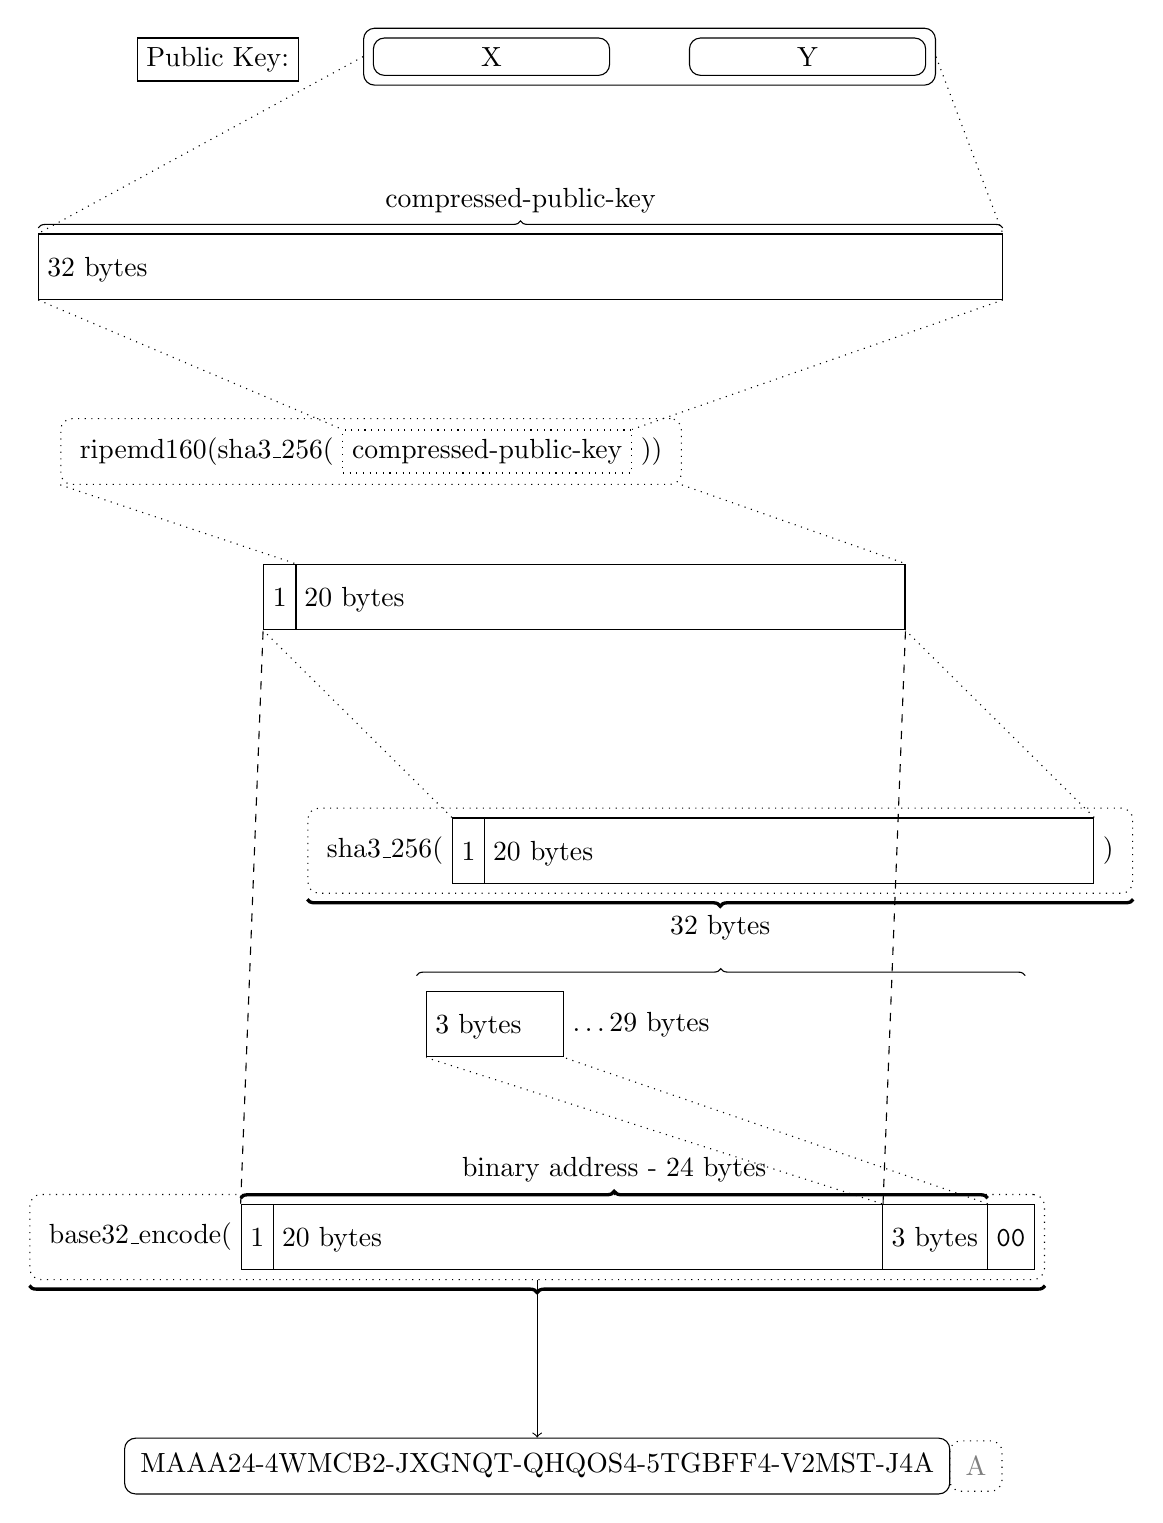
\begin{tikzpicture}[node distance=-\pgflinewidth]
	%%% first row, public key
	\node[draw,anchor=north west] (pubkeyLabel) at (0,0) {Public Key: };

	\node[crou,anchor=north west,minimum width=3cm] (pkx) at (3, 0) {X};
	\node[crou,minimum width=3cm, right=1cm of pkx] (pky) {Y};

	\node[fit=(pkx)(pky),crou] (xy) {};

	% join lines
	\node[crecb,below left=2cm and -8cm of pkx,text width=12cm] (bpk32) {32 bytes};

	%%% second row
	\draw[decorate,decoration={brace,raise=2pt}] (bpk32.north west) --
		node[above=4pt] (bpkLabel) {compressed-public-key}
		(bpk32.north east);

	\draw[dotted] (xy.west) -- (bpk32.north west);
	\draw[dotted] (xy.east) -- (bpk32.north east);

	% invisible
	\node[fit=(bpk32)(bpkLabel)] (bpk) {};

	%%% third row - ripeMD
	% it's easier to do it this way, as problems with paths show up when using nested tikzpicture
	\node[below left=1.5cm and -4cm of bpk] (ripeInner) { $\mathfunc{ripemd160}(\mathfunc{sha3\_256}($ };
	\node[right=of ripeInner, draw, dotted,rounded corners=0] (bpkInnerLabel) {compressed-public-key};
	\node[right=of bpkInnerLabel] (ripeInner2) { $)) $ };

	\node[fit=(ripeInner)(bpkInnerLabel)(ripeInner2), draw, dotted, rounded corners] (ripe) {};

	\draw[dotted] (bpk32.south west) -- (bpkInnerLabel.north west);
	\draw[dotted] (bpk32.south east) -- (bpkInnerLabel.north east);

	%%% fourth row - network byte + ripemd output
	\node[crecb,below left=1cm and -3cm of ripe] (brmd1) {1};
	\node[crecb,right=of brmd1,text width=7.5cm] (brmd20) {20 bytes};

	\draw[dotted] (ripe.south west) -- (brmd20.north west);
	\draw[dotted] (ripe.south east) -- (brmd20.north east);

	%%% fifth row - SHA3(version + ripe)
	\node[below left=2.5cm and -2cm of brmd20] (checkInner) { $\mathfunc{sha3\_256(}$ };
	\node[crecb,right=of checkInner] (bInnerRmd1) {1};
	\node[crecb,right=of bInnerRmd1,text width=7.5cm] (bInnerRmd20) {20 bytes};
	\node[right=of bInnerRmd20] (checkInner2) { $) $ };

	\draw[dotted] (bInnerRmd1.north west) -- (brmd1.south west);
	\draw[dotted] (bInnerRmd20.north east) -- (brmd20.south east);

	\node[fit=(checkInner)(bInnerRmd1)(bInnerRmd20)(checkInner2), draw, dotted, rounded corners] (check) {};

	\draw[decorate,decoration={brace,mirror,raise=2pt},very thick] (check.south west) -- node[below=4pt] (check32) {32 bytes} (check.south east);

	%%% sixth row - sha3 output
	\node[below=1.5cm of bInnerRmd20,text width=5.5cm] (check29) {\ldots 29 bytes};
	\node[crecb,left=of check29,text width=1.5cm] (check3) {3 bytes};
	\node[fit=(check3)(check29)] (checkGroup) {};
	\draw[decorate,decoration={brace,raise=2pt}] (checkGroup.north west) -- (checkGroup.north east);

	%%% seventh row - binary address
	\node[crecb,below left=2cm and -6cm of check29] (bAddr0) {\texttt{00}};
	\node[crecb,left=of bAddr0] (bAddr3) {3 bytes};
	\node[crecb,left=of bAddr3,text width=7.5cm] (bAddr20) {20 bytes};
	\node[crecb,left=of bAddr20] (bAddr1) {1};

	\node[left=of bAddr1] (base32) { $\mathfunc{base32\_encode(}$ };

	\node[fit=(bAddr1)(bAddr20)(bAddr3)] (binaryAddress) {};

	\node[fit=(base32)(bAddr1)(bAddr20)(bAddr3)(bAddr0), draw, dotted, rounded corners] (base32call) {};

	\draw[decorate,decoration={brace,raise=2pt},very thick] (bAddr1.north west) -- node[above=4pt] {binary address - 24 bytes} (bAddr3.north east);
	\draw[decorate,decoration={brace,mirror,raise=2pt},very thick] (base32call.south west) -- node[below=4pt] (binAddr) {} (base32call.south east);

	% final association
	\draw[dotted] (bAddr3.north west) -- (check3.south west);
	\draw[dotted] (bAddr3.north east) -- (check3.south east);

	\draw[dashed,thin] (bAddr1.north west) -- (brmd1.south west);
	\draw[dashed,thin] (bAddr20.north east) -- (brmd20.south east);

	\node[draw,below=2cm of base32call,rounded corners,solid,inner sep=0.2cm] (nanemo) {MAAA24-4WMCB2-JXGNQT-QHQOS4-5TGBFF4-V2MST-J4A};
	\node[draw,right=of nanemo,dotted,rounded corners,inner sep=0.2cm] (nanemotrim) {\textcolor{gray}{A}};
	\draw[solid,thin,->] (base32call.south) -- (nanemo.north);
\end{tikzpicture}

	}{Address generation}
\end{figure}

\pagebreak

\subsection{Address Aliases}
\index{alias address}
An address can have one or more aliases assigned using an address alias transaction\nemtechdocsfootnote{concepts/namespace.html\#addressaliastransaction}.
All transactions accepting addresses support using either a public key derived address or an address alias.
In case of such transactions, the format of the address alias field is:
\begin{itemize}
	\item{network byte ORed with value 1}
	\item{8 byte namespace id that is an alias}
	\item{16 zero bytes}
\end{itemize}

\subsection{Intentional Address Collision}
It is possible that two different public keys will yield the same address.
If such an address contains any valuable assets \textbf{AND} has not been associated with a public key earlier (for example, by sending a transaction from the account), it would be possible for an attacker to withdraw funds from such an account.

In order for the attack to succeed, the attacker would need to find a private+public keypair such that the SHA3\_256 of the public key would \textbf{at the same time} be equal to the RIPEMD\_160 preimage of the 160-bit hash mentioned above.
Since SHA3\_256 offers 128 bits of security, it is mathematically improbable for a single SHA3\_256 collision to be found.
Due to similarities between \codenamespace addresses and Bitcoin addresses, the probability of causing a \codenamespace address collision is roughly the same as that of causing a Bitcoin address collision.

	\section{Transactions}
\label{sec:transactions}

\nemquote{%
In fact, a large part of what we think of as economic activity is designed to accomplish what high transaction costs would otherwise prevent or to reduce transaction costs so that individuals can negotiate freely and we can take advantage of that diffused knowledge of which Friedrich Hayek has told us.
}{Ronald Coase}

\nemchapterfirstletter{T}{ransactions} are instructions that modify the global chain state.
They are processed atomically and grouped into blocks.
If any part of a transaction fails processing, the global chain state is reset to the state prior to the transaction application attempt.

There are two fundamental types of transactions: basic transactions and aggregate transactions.
Basic transactions represent a single operation and require a single signature.
Aggregate transactions are containers of one or more transactions that may require multiple signatures.

Aggregate transactions allow basic transactions to be combined into potentially complex operations and executed atomically.
This increases developer flexibility relative to a system that only guarantees atomicity for individual operations while still constraining the global set of operations allowed to a finite set.
It does not require the introduction of a Turing-complete language and all of its inherent disadvantages.
Developers do not need to learn any new languages nor develop bespoke contract implementations from scratch.
The composition of transactions should be less error-prone and lead to fewer bugs than implementing computationally complete programs.

\subsection{Basic Transaction}

A basic transaction is composed of both cryptographically verifiable and unverifiable data.
All verifiable data is contiguous and is signed by the transaction signer.
All unverifiable data is either ignored (e.g. padding bytes) or deterministically computable from verifiable data.
Each basic transaction requires verification of exactly one signature.

None of the unverifiable header fields need to be verified.
\field{Size} is the serialized size of the transaction and can always be derived from verifiable transaction data.
\field{Signature} is an output from signing and an input to verification.
\field{SignerPublicKey} is an input to both signing and verification.
In order for a transaction $T$ to pass signature verification, both \field{Signature} and \field{SignerPublicKey} must be matched with the verifiable data, which has a length relative to \field{Size}.
$$\mathfunc{verify}(\structField{T}{Signature}, \structField{T}{SignerPublicKey}, \mathfunc{VerifiableDataBuffer}(T))$$

\field{Reserved} bytes are used for padding transactions so that all integral fields and cryptographic primitives have natural alignment.
Since these bytes are meaningless, they can be stripped without invalidating any cryptographic guarantees.

Binary layouts for all transaction types are specified in \codename's open source schema language
\footnote{Schemas can be found at https://github.com/nemtech/catbuffer.}.
Please refer to the published schemas for the most up to date specifications.

\begin{figure}[H]
	\nemcenterwithcaption{
		\begin{subfigure}{.5\textwidth}
			\nemmemorylayout{
				\begin{leftwordgroup}{\texttt{0x00}}
					\bitbox{4}{Size} \bitbox{4}{Reserved}
				\end{leftwordgroup} \\
				\nemmemorymultiwordbox{0x08}{Signature}{7} \\
				\nemmemorymultiwordbox{0x48}{SignerPublicKey}{3} \\
				\begin{leftwordgroup}{\texttt{0x68}}
					\bitbox{4}{Reserved} \bitbox[]{4}{}
				\end{leftwordgroup}
			}{Header (unsigned)}
		\end{subfigure}%
		\begin{subfigure}{.5\textwidth}
			\nemmemorylayout{
				\begin{leftwordgroup}{\texttt{0x6C}}
					\bitbox[br]{4}{} \bitbox{4}{V, N, T}
				\end{leftwordgroup} \\
				\nemmemorysinglewordbox{0x70}{MaxFee} \\
				\nemmemorysinglewordbox{0x78}{Deadline} \\
				\nemmemorymultiwordboxskipped{0x80}{Payload}{}
			}{Verifiable data}
		\end{subfigure}
	}{Basic transaction binary layout}
\end{figure}

In figures, \texttt{(V)ersion}, \texttt{(N)etwork} and \texttt{(T)ype} are abbreviated due to space concerns.

\subsection{Aggregate Transaction}
\label{sec:transactions:aggregate}

The layout of an aggregate transaction is more complex than that of a basic transaction, but there are some similarities.
An aggregate transaction shares the same unverifiable header as a basic transaction, and this data is processed in the same way.
Additionally, an aggregate transaction has a footer of unverifiable data followed by embedded transactions and cosignatures.

An aggregate transaction can always be submitted to the network with all requisite cosignatures.
In this case, it is said to be \emph{complete} and it is treated like any other transaction without any special processing.

API nodes can also accept \emph{bonded} aggregate transactions that have incomplete cosignatures.
The submitter must pay a bond that is returned if and only if all requisite cosignatures are collected before the transaction times out.
Assuming this bond is paid upfront, an API node will collect cosignatures associated with this transaction until it either has sufficient signatures or times out.

\field{TransactionsHash} is the most important field in an aggregate transaction.
It is the Merkle root hash of the hashes of the embedded transactions stored within the aggregate.
In order to compute this field, a Merkle tree is constructed by adding each embedded transaction hash in natural order.
The resulting root hash is assigned to this field.

None of the unverifiable footer fields need to be verified.
\field{PayloadSize} is a computed size field that must be correct in order to extract the exact same embedded transactions that were used to calculate \field{TransactionsHash}.
\field{Reserved} bytes, again, are used for padding and have no intrinsic meaning.

\begin{figure}[H]
	\nemcenterwithcaption{
		\begin{subfigure}{.33\textwidth}
			\nemmemorylayout{
				\begin{leftwordgroup}{\texttt{0x00}}
					\bitbox{4}{Size} \bitbox{4}{Reserved}
				\end{leftwordgroup} \\
				\nemmemorymultiwordbox{0x08}{Signature}{7} \\
				\nemmemorymultiwordbox{0x48}{SignerPublicKey}{3} \\
				\begin{leftwordgroup}{\texttt{0x68}}
					\bitbox{4}{Reserved} \bitbox[]{4}{}
				\end{leftwordgroup}
			}{Header (unsigned)}
		\end{subfigure}%
		\begin{subfigure}{.33\textwidth}
			\nemmemorylayout{
				\begin{leftwordgroup}{\texttt{0x6C}}
					\bitbox[br]{4}{} \bitbox{4}{V, N, T}
				\end{leftwordgroup} \\
				\nemmemorysinglewordbox{0x70}{MaxFee} \\
				\nemmemorysinglewordbox{0x78}{Deadline} \\
				\nemmemorysinglewordbox{0x80}{TransactionsHash}
			}{Verifiable data}
		\end{subfigure}%
		\begin{subfigure}{.33\textwidth}
			\nemmemorylayout{
				\begin{leftwordgroup}{\texttt{0x88}}
					\bitbox{4}{\tiny PayloadSize} \bitbox{4}{Reserved}
				\end{leftwordgroup} \\
				\nemmemorymultiwordboxskipped{0x90}{Embedded}{Transactions} \\
				\nemmemorymultiwordboxskipped{}{Cosignatures}{}
			}{Unverifiable footer}
		\end{subfigure}
	}{Aggregate transaction header binary layout}
\end{figure}

\subsubsection{Embedded Transaction}

An embedded transaction is a transaction that is contained within an aggregate transaction.
Compared to a basic transaction, the header is smaller, but the transaction-specific data is the same.
\field{Signature} is removed because all signature information is contained in cosignatures.
\field{MaxFee} and \field{Deadline} are removed because they are specified by the parent aggregate transaction.

Client implementations can use the same code to construct the custom parts of either a basic or embedded transaction.
The only difference is in the creation and application of different headers.

Not all transactions are supported as embedded transactions.
For example, an aggregate transaction cannot be embedded within another aggregate transaction.

\begin{figure}[H]
	\nemcenterwithcaption{
		\begin{subfigure}{.5\textwidth}
			\nemmemorylayout{
				\begin{leftwordgroup}{\texttt{0x00}}
					\bitbox{4}{Size} \bitbox{4}{Reserved}
				\end{leftwordgroup} \\
				\nemmemorymultiwordbox{0x08}{SignerPublicKey}{3} \\
				\begin{leftwordgroup}{\texttt{0x28}}
					\bitbox{4}{Reserved} \bitbox[]{4}{}
				\end{leftwordgroup}
			}{Header (unsigned)}
		\end{subfigure}%
		\begin{subfigure}{.5\textwidth}
			\nemmemorylayout{
				\begin{leftwordgroup}{\texttt{0x2C}}
					\bitbox[br]{4}{} \bitbox{4}{V, N, T}
				\end{leftwordgroup} \\
				\nemmemorymultiwordboxskipped{0x30}{Payload}{}
			}{Verifiable data}
		\end{subfigure}
	}{Embedded transaction binary layout}
\end{figure}

\subsubsection{Cosignature}

A cosignature is a pair composed of a public key and its corresponding signature.
Zero or more cosignatures are appended at the end of an aggregate transaction.
Cosignatures are used to cryptographically verify an aggregate transaction involving multiple parties.

\begin{figure}[H]
	\nemcenter{
		\nemmemorylayout{
			\nemmemorymultiwordbox{0x00}{SignerPublicKey}{3} \\
			\nemmemorymultiwordbox{0x20}{Signature}{7}
		}{Cosignature binary layout}
	}{}
\end{figure}

In order for an aggregate transaction $A$ to pass verification, it must pass basic transaction signature verification and have a cosignature for every embedded transaction signer
\footnote{In the case of multisignature accounts, there must be enough cosignatures to satisfy the multisignature account constraints.}.

Like any transaction, an aggregate transaction, must pass basic transaction signature verification.
$$\mathfunc{verify}(\structField{A}{Signature}, \structField{A}{SignerPublicKey}, \mathfunc{VerifiableDataBuffer}(A))$$

Additionally, all cosignatures must pass signature verification.
Notice that cosigners sign the hash of an aggregate transaction data, not the data directly.
$$\sum_{0\leq i \leq N_C} \mathfunc{verify}(\structField{C}{Signature}, \structField{C}{SignerPublicKey}, \hf(\mathfunc{VerifiableDataBuffer}(A)))$$

Finally, there must be a cosignature that corresponds to and satisfies each embedded transaction signer.

\subsubsection{Extended Layout}

The aggregate transaction layout described earlier was correct with one simplification.
All embedded transactions are padded so that they end on 8-byte boundaries.
This ensures that all embedded transactions and cosignatures begin on 8-byte boundaries as well.
The padding bytes are never signed nor included in any hashes.

\begin{figure}[H]
	\nemcenter{
		\nemmemorylayout{
			\begin{leftwordgroup}{}
				\bitbox{4}{\tiny PayloadSize} \bitbox{4}{Reserved}
			\end{leftwordgroup} \\
			\nemmemorymultiwordboxskipped{}{Embedded}{Transaction 1} \\
			\nemmemorysinglewordbox{}{\emph{optional} padding} \\
			\nemmemorymultiwordboxskipped{}{Embedded}{Transaction 2} \\
			\nemmemorysinglewordbox{}{\emph{optional} padding} \\
			\nemmemorymultiwordboxskipped{}{Cosignatures}{}
		}{Aggregate transaction footer with padding}
	}
\end{figure}

\subsection{Transaction Hashes}

Each transaction has two associated hashes - an \emph{entity hash} and a \emph{Merkle component hash}.
The former uniquely identifies a transaction and is used to prevent multiple confirmations of the same transaction.
The latter is more specific and is used when calculating \field{TransactionsHash} \nemrefparens{sec:transactions:aggregate}.

A transaction's entity hash is always calculated as the hash of its verifiable data.
All confirmed transactions must have a unique entity hash.
An aggregate transaction's entity hash is independent of its cosignatures.
This prevents the same aggregate transaction from being confirmed multiple times with different sets of valid cosignatures.

A regular transaction's Merkle component hash is identical to its entity hash.
An aggregate transaction's Merkle component hash is calculated by hashing its entity hash concatenated with all the public keys of its cosignatures
\footnote{Cosignature signatures are not included because they can only have a single value given a specific public key and payload.}.
This ensures that \field{TransactionsHash} reflects all cosignatures that allowed the confirmation of an aggregate transaction.

	\section{Blocks}
\label{sec:blocks}

\nemquote{%
A stumbling block to the pessimist is a stepping-stone to the optimist.
}{Eleanor Roosevelt}

\codenamechapterfirstword is, at its core, a blockchain.
A blockchain is an ordered collection of blocks.
Understanding the parts of a \codenamespace block is fundamental to understanding the platform's capabilities.

The layout of a block is similar to the layout of an aggregate transaction \nemrefparens{sec:transactions:aggregate}.
A block shares the same unverifiable header as an aggregate transaction, and this data is processed in the same way.
Likewise, a block has a footer of unverifiable data followed by transactions.
Unlike an aggregate transaction, a block is followed by basic - not embedded - transactions, and each transaction within a block is signed independently of the block signer\footnote{
In an aggregate transaction, the account creating the aggregate transaction must sign the transaction's data in order for it to be valid.
In a block, the block signer does not need to sign the data of any transaction contained within it.
}.
This allows any transaction satisfying all conditions to be included in any block.

None of the unverifiable footer fields need to be verified.
\texttt{Reserved} bytes are used for padding and have no intrinsic meaning.

\begin{figure}
	\nemcenterwithcaption{
		\begin{subfigure}{.33\textwidth}
			\nemmemorylayout{
				\begin{leftwordgroup}{\texttt{0x00}}
					\bitbox{4}{Size} \bitbox{4}{Reserved}
				\end{leftwordgroup} \\
				\nemmemorymultiwordbox{0x08}{Signature}{7} \\
				\nemmemorymultiwordbox{0x48}{SignerPublicKey}{3} \\
				\begin{leftwordgroup}{\texttt{0x68}}
					\bitbox{4}{Reserved} \bitbox[]{4}{}
				\end{leftwordgroup}
			}{Header (unsigned)}
		\end{subfigure}%
		\begin{subfigure}{.33\textwidth}
			\nemmemorylayout{
				\begin{leftwordgroup}{\texttt{0x6C}}
					\bitbox[br]{4}{} \bitbox{4}{V, N, T}
				\end{leftwordgroup} \\
				\nemmemorysinglewordbox{0x70}{Height} \\
				\nemmemorysinglewordbox{0x78}{Timestamp} \\
				\nemmemorysinglewordbox{0x80}{Difficulty} \\
				\nemmemorymultiwordbox{0x88}{PreviousBlockHash}{3} \\
				\nemmemorymultiwordbox{0xA8}{TransactionsHash}{3} \\
				\nemmemorymultiwordbox{0xC8}{ReceiptsHash}{3} \\
				\nemmemorymultiwordbox{0xE8}{StateHash}{3} \\
				\nemmemorymultiwordbox{0x108}{\small BeneficiaryPublicKey}{3} \\
				\begin{leftwordgroup}{\texttt{0x128}}
					\bitbox{4}{\tiny FeeMultiplier} \bitbox[]{4}{}
				\end{leftwordgroup}
			}{Verifiable data}
		\end{subfigure}%
		\begin{subfigure}{.33\textwidth}
			\nemmemorylayout{
				\begin{leftwordgroup}{\texttt{0x12C}}
					\bitbox[br]{4}{} \bitbox{4}{Reserved}
				\end{leftwordgroup} \\
				\nemmemorymultiwordboxskipped{0x130}{Transactions}{}
			}{Unverifiable footer}
		\end{subfigure}
	}{Block header binary layout}
\end{figure}

\subsection{Block Fields}

\field{Height} is the block sequence number.
The first block, called the \nind{nemesis block}\index{block!nemesis}, has a height of one.
Each successive block increments the height of the previous block by one.

\field{Timestamp} is the number of milliseconds that have elapsed since the nemesis block.
Each successive block must have a timestamp greater than that of the previous blocks because block time is strictly increasing.
Each network tries to keep the average time between blocks close to \nind{target block time}.

\field{Difficulty} determines how hard is to harvest a new block, based on previous blocks.
Difficulty is described in detail in \nemref{sec:blockchain:difficulty}.

\field{PreviousBlockHash} is the hash of the previous block.
This is used to guarantee that all blocks within a blockchain are linked and deterministically ordered.

\field{TransactionsHash} is the merkle root hash of the hashes of the transactions stored within the block
\footnote{This field has the same purpose as the identically named field in an aggregate transaction.}.
In order to compute this field, a merkle tree is constructed by adding each transaction hash in natural order.
The resulting root hash is assigned to this field.

\field{ReceiptsHash} is the merkle root hash of the hashes of the receipts produced while processing the block.
When a network is configured without \nemsetting{network}{enableVerifiableReceipts}, this field must be zeroed in all blocks \nemrefparens{sec:blocks:receipts}.

\field{StateHash} is the hash of the global blockchain state after processing the block.
When a network is configured without \nemsetting{network}{enableVerifiableState}, this field must be zeroed in all blocks.
Otherwise, it's calculated as described in \nemref{sec:blocks:statehash}.

\field{BeneficiaryPublicKey} is the account that will be allocated the block's beneficiary share when the network has a nonzero \nemsetting{network}{harvestBeneficiaryPercentage}.
This field can be set to any account, even one that isn't yet known to the network.
This field is set by the node owner when a new block is harvested.
If this account is set to one owned by the node owner, the node owner will share in fees paid in all blocks harvested on its node.
This, in turn, incentivizes the node owner to run a strong node with many delegated harvesters.

\field{FeeMultiplier} is a multiplier that is used to calculate the effective fee of each transaction contained within a block.
The \nemsetting{node}{minFeeMultiplier} is set by the node owner and can be used to accomplish varying goals, including maximization of profits or confirmed transactions.
Assuming a block $B$ containing a transaction $T$, the effective transaction fee can be calculated as:
$$\mathfunc{effectiveFee}(T) = \structField{B}{FeeMultiplier} \cdot \mathfunc{sizeof}(T)$$
If the effective fee is greater than the transaction \field{MaxFee}, the transaction signer keeps the difference.
Only the effective fee is deducted from the transaction signer and credited to the harvester.
Further information about fee multipliers can be found in\nemref{sec:blockchain:generation}.

\subsection{Receipts}
\label{sec:blocks:receipts}

During the execution of a block, zero or more receipts are generated.
Receipts are primarily used to communicate state changes triggered by side effects to clients.
In this way, they allow simpler clients to still be aware of complex state changes.

For example, a namespace expiration is triggered by the number of blocks that have been confirmed since the namespace was created.
While the triggering event is in the blockchain, there is no indication of this state change in the block at which the expiration occurs.
Without receipts, a client would need to keep track of all namespaces and expiration heights.
With receipts, a client merely needs to monitor for expiration receipts.

Another example is around harvest rewards.
Receipts are produced that indicate the main - not delegated - account that gets credited and any beneficiary splits.
They also communicate the amount of currency created by inflation.

Receipts are grouped into three different types of statements and collated by receipt sources.
The three types of statements are transaction, address resolution and mosaic resolution.

\subsubsection{Receipt Source}

Each part of a block that is processed is assigned a two-part block-scoped identifier.
The source (0, 0) is always used to identify block-triggered events irrespective of the number of transactions in a block.

\begin{table}[ht]
	\nemcenterwithcaption{
		\begin{tabular}{|p{0.20\linewidth}|p{0.40\linewidth}|p{0.40\linewidth}|}
			\hline
			Source & Primary Id & Secondary Id \\
			\hline
			Block & 0 & 0 \\
			Transaction & 1-based index within the block & 0 \\
			Embedded Transaction & 1-based index of containing aggregate within the block & 1-based index within the aggregate \\
			\hline
		\end{tabular}
	}{Receipt source values}
\end{table}

\subsubsection{Transaction Statement}

Transaction statements are used to group receipts that have a shared receipt source.
Each statement is composed of a receipt source and one or more receipts.
Accordingly, each receipt source that generates a receipt will have exactly one corresponding transaction statement.

\begin{figure}[H]
	\nemcenterwithcaption{
		\begin{subfigure}{.5\textwidth}
			\nemmemorylayout{
				\begin{leftwordgroup}{\texttt{0x00}}
					\bitbox{4}{Size} \bitbox{2}{V} \bitbox{2}{T}
				\end{leftwordgroup} \\
				\nemmemorysinglewordbox{0x08}{ReceiptSource} \\
				\nemmemorymultiwordboxskipped{0x10}{Receipts}{}
			}{Transaction statement binary layout}
		\end{subfigure}%
		\begin{subfigure}{.5\textwidth}
			\nemmemorylayout{
				\begin{leftwordgroup}{\texttt{0x00}}
					\bitbox{4}{Size} \bitbox{2}{V} \bitbox{2}{T}
				\end{leftwordgroup} \\
				\nemmemorymultiwordboxskipped{0x08}{Payload}{}
			}{Receipt binary layout}
		\end{subfigure}
	}{Transaction statement layout}
\end{figure}

Transaction statement data is not padded because it is only written during processing and never read, so padding yields no server performance benefit.
A transaction statement hash is constructed by concatenating and hashing all statement data excepting \field{Size} fields, which are derivable from other data.

\subsubsection{Resolution Statements}

Resolution statements are used exclusively for indicating alias resolutions.
They allow a client to always resolve an unresolved value even when it changes within a block.
Theoretically, two unresolved aliases within the same block could resolve to different values if there is an alias change between their usages.
Each statement is composed of an unresolved value and one or more resolutions in order to support this.

There are two types of resolution statements - address and mosaic - corresponding to the two types of aliases.
Although \autoref{fig:blocks:mosaicResolutionStatementLayout} illustrates the layout of a mosaic resolution statement, the layout of an address resolution statement is nearly identical.
The only difference is that the resolved and unresolved values are 25-byte addresses instead of 8-byte mosaic ids.

\begin{figure}[H]
	\nemcenterwithcaption{
		\begin{subfigure}{.5\textwidth}
			\nemmemorylayout{
				\begin{leftwordgroup}{\texttt{0x00}}
					\bitbox{4}{Size} \bitbox{2}{V} \bitbox{2}{T}
				\end{leftwordgroup} \\
				\nemmemorysinglewordbox{0x08}{\small MosaicId Unresolved} \\
				\nemmemorymultiwordboxskipped{0x10}{Resolution}{Entries}
			}{Mosaic resolution statement binary layout}
		\end{subfigure}%
		\begin{subfigure}{.5\textwidth}
			\nemmemorylayout{
				\begin{leftwordgroup}{\texttt{0x00}}
					\bitbox{8}{ReceiptSource}
				\end{leftwordgroup} \\
				\begin{leftwordgroup}{\texttt{0x08}}
					\bitbox{8}{\small MosaicId Resolved}
				\end{leftwordgroup}
			}{Resolution entry binary layout}
		\end{subfigure}
	}{Mosaic resolution statement layout\label{fig:blocks:mosaicResolutionStatementLayout}}
\end{figure}

Resolution statement data is not padded because it is only written during processing and never read, so padding yields no server performance benefit.
A resolution statement hash is constructed by concatenating and hashing all statement data excepting \field{Size} fields, which are derivable from other data.

It is important to note that a resolution statement is only produced when a resolution occurs.
If an alias is registered or changed in a block, but not used in that block, no resolution statement will be produced.
However, a resolution statement will be produced by each block that contains that alias and requires it to be resolved.

\subsubsection{Receipts Hash}
\label{sec:blocks:receiptshash}

In order to calculate a block's receipt hash, first all statements generated during block processing are collected.
Then a merkle tree is created by adding all statement hashes in the following order:

\begin{enumerate}
	\item{Hashes of transaction statements ordered by receipt source.}
	\item{Hashes of address resolution statements ordered by unresolved address.}
	\item{Hashes of mosaic resolution statements ordered by unresolved mosaic id.}
\end{enumerate}

When a network is configured with \nemsetting{network}{enableVerifiableReceipts}, the root hash of this merkle tree is set as the block's \field{ReceiptHash}.
A client can perform a merkle proof to prove a particular statement was produced during the processing of a specific block.

\subsection{State Hash}
\label{sec:blocks:statehash}

\codenamespace stores the global blockchain state across multiple typed state repositories.
For example, the account state is stored in one repository and the multsignature state is stored in another.
Each repository is a simple key value store.
The specific repositories present in a network are determined by the transaction plugins enabled by that network.

When a network is configured with \nemsetting{network}{enableVerifiableState}, a patricia tree is created for each repository.
This produces a single hash that deterministically fingerprints each repository.
Accordingly, assuming $N$ repositories, $N$ hashes deterministically fingerprint the global blockchain state.

It is possible to store all $N$ hashes directly in each block header, but this is undesirable.
Each block header should be as small as possible because all clients, minimally, need to sync all headers to verify a chain is rooted to the nemesis block.
Additionally, adding or removing functionality could change the number of repositories ($N$) and the format of the block header.

Instead, all root hashes are concatenated\footnote{The concatenation order is fixed and determined by the repository id.} and hashed to calculate the \field{StateHash},
which is a single hash that deterministically fingerprints the global blockchain state.
\begin{align*}
	\mathvar{RepositoryHashes} = \: & 0 \\
	\mathvar{RepositoryHashes} = \: & \sum_{0\leq i \leq N} \mathfunc{concat}(\mathvar{RepositoryHashes}, \mathvar{RepositoryHash}_i) \\
	\mathvar{StateHash} = \: & \hf(\mathvar{RepositoryHashes})
\end{align*}

\subsection{Extended Layout}

The block layout described earlier was correct with one simplification\footnote{
This is consistent with the extended layout of an aggregate transaction as well.}.
All transactions are padded so that they end on 8-byte boundaries.
This ensures that all transactions begin on 8-byte boundaries as well.
The padding bytes are never signed nor included in any hashes.

\begin{figure}[H]
	\nemcenter{
		\nemmemorylayout{
			\begin{leftwordgroup}{}
				\bitbox[br]{4}{} \bitbox{4}{Reserved}
			\end{leftwordgroup} \\
			\nemmemorymultiwordboxskipped{}{Transaction 1}{} \\
			\nemmemorysinglewordbox{}{\emph{optional} padding} \\
			\nemmemorymultiwordboxskipped{}{Transaction 2}{} \\
			\nemmemorysinglewordbox{}{\emph{optional} padding}
		}{Block transaction footer with padding}
	}
\end{figure}

	\section{Blockchain}
\label{sec:blockchain}

\nemquote{%
It is a mistake to look too far ahead.
Only one link of the chain of destiny can be handled at a time.
}{Winston Churchill}

\codenamespace is centered around a public ledger called the blockchain that links blocks together.
The complete transaction history is held in the blockchain.
All blocks, and transactions within blocks, are deterministically and cryptographically ordered.
The maximum number of transactions per block can be configured per-network.

\subsection{Block Difficulty}
\index{block!difficulty}
\label{sec:blockchain:difficulty}

The nemesis block has a predefined \nind{initial difficulty} of $10^{14}$.
All difficulties are clamped between a minimum of $10^{13}$ and a maximum of $10^{15}$.

The difficulty for a new block is derived from the difficulties and timestamps of the most recently confirmed blocks.
The number of blocks taken into consideration is configurable per-network.

If less than \nemsetting{network}{maxDifficultyBlocks} are available, only those available are taken into account.
Otherwise, the difficulty is calculated from the last $n$ blocks in the following way:
\begin{align*}
	\tag{average difficulty} d &= \frac{1}{n}\sum_{i=1}^n (\text{difficulty of $block_i$}) \\
	\tag{average creation time} t &= \frac{1}{n}\sum_{i=1}^n (\text{time to create $block_i$}) \\
	\tag{new difficulty} \mathvar{difficulty} &= d \; \frac{\nemsetting{network}{blockGenerationTargetTime}}{t}
\end{align*}

This algorithm produces blocks with an average time close to the desired \nemsetting{network}{blockGenerationTargetTime} network setting.

If the new difficulty is more than 5\% larger or smaller than the difficulty of the last block, then the change is capped to 5\%.
The maximum change rate of 5\% per block makes it hard for an attacker with considerably less than 50\% importance to create a better chain in secret.
Since difficulty is roughly correlated with the total amount of importance currently harvesting, the attacker's secret chain will necessarily have a much lower difficulty.
Limiting the maximum difficulty decrease per block means the attacker's chain will quickly fall behind the main chain.
By the time the difficulty adjusts to something more proportional to the attacker's importance, the main chain will be far ahead.
Block times will be considerably higher than \nemsetting{network}{blockGenerationTargetTime} at the beginning of the attacker's secret chain.

\begin{figure}
	\begin{tikzpicture}
		\begin{axis}[
				grid = major,
				grid style={dashed, gray!30},
				xmin=5500, xmax=35500,
				ymin=12, ymax=18,
				width=15cm, height=8cm,
				xlabel=block height,
				ylabel=seconds,
				legend style={at={(0.05, 0.98)}, anchor=north west, draw=none},
				scaled x ticks = false,
				xtick distance=3000
			]
			% this must be before the plot itself
			\addlegendimage{no markers,nemgreen}
			\addplot[color=nemgreen] table [mark=none, x=height, y=avg blocktime, col sep=comma] {data/avgblocktimes.csv};
			\legend{block times average over 49 blocks}
		\end{axis}
	\end{tikzpicture}
	\caption{Dev network average block times, with target block time = 15s}
\end{figure}

\subsection{Block Score}
\label{sec:blockchain:blockScore}
\index{block!score}
\label{sec:blockchain:score}

The score for a block is derived from its difficulty and the time (in seconds) that has elapsed since the last block:
\begin{equation}
	\tag{block score} \mathvar{score} = \mathvar{difficulty} - \mathname{time elasped since last block}
\end{equation}

\subsection{Block Generation}
\label{sec:blockchain:generation}
\index{block!generation}

The process of creating new blocks is called \nind{harvesting}.
The harvesting account gets the fees from the transactions it includes in a block.
This gives the harvester an incentive to create a valid block and add as many transactions to it as possible.

An account is eligible to harvest if all of the following are true:
\begin{enumerate}
	\item{Importance score at the last importance recalculation height is nonzero.}
	\item{Balance no less than a network defined \nemsetting{network}{minHarvesterBalance}.}
	\item{
		Balance no greater than a network defined \nemsetting{network}{maxHarvesterBalance}
		\footnote{This feature is primarily intended to prevent core funds and exchange accounts from harvesting.}.
	}
\end{enumerate}

An account owner can delegate its importance to some other account\nemtechdocsfootnote{concepts/harvesting.html\#accountlinktransaction} in order to avoid exposing a private key with funds.

The actual reward a harvester receives is customizable based on network settings.
If \nemsetting{inflation}{inflation} configuration has nonzero values, each harvested block may contain an additional inflation block reward.
This makes harvesting more profitable.
If harvesting fee sharing is enabled (via \nemsetting{network}{harvestBeneficiaryPercentage}), the harvester will forfeit a share of fees to the node hosting its harvesting key.
This makes running network nodes more profitable but harvesting less profitable.

\index{block!fee multiplier}

Each block must specify a \emph{fee multiplier} that determines the effective fee that must be paid by all transactions included in that block.
Typically, the node owner sets the \nemsetting{node}{minFeeMultiplier} that applies to all blocks harvested by the node.
Only transactions that satisfy the following will be allowed to enter that node's unconfirmed transactions cache and be eligible for inclusion into blocks harvested by that node:
\begin{equation}
	\mathname{transaction max fee} \geqslant \nemsetting{node}{minFeeMultiplier} \cdot \mathname{transaction size (bytes)}
\end{equation}

Rejected transactions may still be included in blocks harvested by other nodes with lower requirements.
The specific algorithm used to select transactions for inclusion in harvested blocks is configured by the \nemsetting{node}{transactionSelectionStrategy} setting.
\codenamespace offers three built-in selection strategies
\footnote{In all cases, all available transactions must already fulfill the requirement that \nemsetting{node}{minFeeMultiplier} indicates.}:

\begin{enumerate}
	\item{\texttt{oldest}: \\
		This is the least resource-intensive strategy and is recommended for high TPS networks.
		Transactions are added to a new block in the order in which they have been received.
		This ensures that the oldest transactions are selected first and attempts to minimize the number of transactions timing out.
		As a consequence, this strategy is rarely profit maximizing for the harvester.
	}
	\item{\texttt{maximize-fee}: \\
		Transactions are selected in such a way that the cumulative fee for all transactions in a block is maximized.
		A greedy node will pick this strategy.
		Maximizing the total block fee does not necessarily mean that the number of transactions included is maximized as well.
		In fact, in many cases, the harvester will only include a subset of the transactions that are available.
	}
	\item{\texttt{minimize-fee}: \\
		Transactions with the lowest maximum fee multipliers are selected first by this strategy.
		Generous nodes will pick this strategy together with a very low \nemsetting{node}{minFeeMultiplier}.
		If this setting is zero, then the harvester will include transactions with zero fees first.
		This allows users to send transactions that get included in the blockchain for free!
		In practice, it is likely that only a few nodes will support this.
		Even with such a subset of nodes running, zero fee transactions will still have the lowest probability of getting included in a block because they will always be supported by the least number of nodes in the network.
	}
\end{enumerate}

Transactions can initiate transfers of both static and dynamic amounts.
Static amounts are fixed and independent of external factors.
For example, the amount specified in a transfer transaction\nemtechdocsfootnote{concepts/transfer-transaction.html} is static.
The exact amount specified is always transfered from sender to recipient.
In contrast, dynamic amounts are variable relative to the average transaction cost.
These are typically reserved for fees paid to acquire unique network artifacts, like namespaces or mosaics.
For such artifacts, a flat fee is undesirable because it would be unresponsive to the market.
Likewise, solely using a single block's \field{FeeMultiplier} is problematic because harvesters could cheat and receive artifacts for free by including registrations in self-harvested blocks with zero fees.
Instead, a dynamic fee multiplier is used.
This multiplier is calculated as the median of the \field{FeeMultiplier} values in the last \nemsetting{network}{maxDifficultyBlocks} blocks.
\nemsetting{network}{defaultDynamicFeeMultiplier} is used when there are not enough values and as a replacement for zero values.
The latter adjustment ensures that the effective amounts are always nonzero.
In order to arrive at the effective amount, the base amount is multiplied by the dynamic fee multiplier.

\begin{align*}
	\mathname{effective amount} = \: & \mathname{base amount} \cdot \mathname{dynamic fee multiplier}
\end{align*}

\index{generation hash}
\index{block!generation hash}

The generation hash of a block is derived from the previous block generation hash and the public key of the current block harvester:
\begin{align*}
	\tag{generation hash}
	\mathfunc{gh}(1) = \: & \nemsetting{network}{generationHash} \\
	\mathfunc{gh}(N) = \: & \hf(\mathfunc{gh}(N - 1), \mathname{public key of account})
\end{align*}

\index{block!hit}
\index{block!target}
To check if an account is allowed to create a new block at a specific network time, the following values are compared:
\begin{itemize}
	\item{$hit$: defines per-block value that needs to be hit.}
	\item{$target$: defines per-harvester power that increases as time since last harvested block increases.}
\end{itemize}

An account is allowed to create a new block whenever $\mathvar{hit} < \mathvar{target}$.
Since $\mathvar{target}$ is proportional to the elapsed time, a new block will be created after a certain amount of time even if all accounts are unlucky and generate a very high hit.

In the case of delegated harvesting, the importance of the original account is used instead of the importance of the delegated account.

The target is calculated as follows
\footnote{The implementation uses 256-bit integer instead of floating point arithmetic in order to avoid any problems due to rounding.}:
\begin{align*}
	\mathvar{multiplier} = \: & 2^{64} \\
	t = \: & \mathname{time in seconds since last block} \\
	b = \: & 8999999998 \: \cdot \: (\mathname{account importance}) \\
	i = \: & \mathname{total chain importance} \\
	d = \: & \mathname{new block difficulty} \\
	\mathvar{target} = \: & \frac{\mathvar{multiplier} \cdot t \cdot b}{i \cdot d}
\end{align*}

\emph{Block time smoothing}\index{block!time smoothing} can be enabled, which results in more stable block times.
If enabled, $multiplier$ above is calculated in the following way
\footnote{
	The implementation uses fixed point instead of floating point arithmetic in order to avoid any problems due to rounding.
	Specificaly, 128-bit fixed point numbers are used where the 112 high bits represent the integer part and the 16 low bits represent the decimal part.
	\texttt{log2(e)} is approximated as \texttt{14426950408 / 10000000000}.
	If the calculated \field{power} is too negative, \field{smoothing} will be set to zero.
}:
\begin{align*}
	\mathvar{factor} = \: & \nemsetting{network}{blockTimeSmoothingFactor} / 1000.0 \\
	\mathvar{tt} = \: & \nemsetting{network}{blockGenerationTargetTime} \\
	\mathvar{power} = \: & factor \cdot \frac{\mathname{time in seconds since last block} - \mathvar{tt}}{\mathvar{tt}} \\
	\mathvar{smoothing} = \: & \min\left(e^{\mathvar{power}}, 100.0\right) \\
	\mathvar{multiplier} = \: & \mathfunc{integer}\left(2^{54} \cdot \mathvar{smoothing}\right) \cdot 2^{10}
\end{align*}

Hit is 64-bit approximation of $2^{54} \left|\ln\left(\frac{\mathvar{gh}}{2^{256}}\right)\right|$, where $\mathvar{gh}$ is a new generation hash
\footnote{
	The implementation uses 128-bit integer instead of floating point arithmetic in order to avoid any problems due to rounding.
	\texttt{log2(e)} is approximated as \texttt{14426950408889634 / 10000000000000000}.
}.

First, let's rewrite value above using $\log$ with base $2$:
$$
\mathvar{hit} = \frac{2^{54}}{\log_2\left(\euler\right)} \cdot \left|\log_2\left(\frac{\mathvar{gh}}{2^{256}}\right)\right|
$$

Note, that $\frac{\mathvar{gh}}{2^{256}}$ is always $< 1$, therefore $\log$ will always yield negative value. \\
Now, $\log_2\left(\frac{\mathvar{gh}}{2^{256}}\right)$, can be rewritten as $\log_2\left(\mathvar{gh}\right) - \log_2\left(2^{256}\right)$. \\

Dropping absolute value and rewriting yields:
\begin{align*}
	\mathvar{scale} = \: & \frac{1}{\log_2\left(\euler\right)} \\
	\mathvar{hit} = \: & \mathvar{scale} \cdot 2^{54} (\log_2\left(2^{256}\right) - \log_2\left(\mathvar{gh}\right))
\end{align*}

This can be further simplified to:
$$
\mathvar{hit} =  \mathvar{scale} \cdot ( 2^{54} \cdot 256 -  2^{54} \cdot \log_2\left(\mathvar{gh}\right))
$$

The implementation approximates the logarithm using only the first 32 non-zero bits of the new generation hash.
There's also additional handling for edge cases.

Also note that $\mathvar{hit}$ has an exponential distribution. Therefore, the probability to create a new block does not change if the importance is split among many accounts.

\subsection{Automatic Delegated Harvester Detection}

When \nemsetting{user}{enableDelegatedHarvestersAutoDetection} is set, the server allows other accounts to register as delegated harvesters via special transfer messages.
The server inspects all transfer messages sent to its \nemsetting{user}{bootPrivateKey} account.
Each message that begins with the magic bytes \texttt{0x98E5BF64C771CCFE} is written out to a file queue for further processing.

Periodically, a scheduled task inspects all queued messages.
Each message is expected to contain a private key for a candidate delegated harvester\footnote{
Please refer to the project code or developer documentation for details about the format of this message.}.
The delegated harvester private key is encrypted with the server's boot public key in order to prevent a malicious actor from intercepting delegated harvester private keys.
Any message that contains unexpected contents is ignored and discarded.

Valid messages are decrypted and processed.
If possible, announced delegated harvester private keys will be used by the server to harvest blocks.
A server can have at most \nemsetting{harvesting}{maxUnlockedAccounts} harvesters.
Upon reaching that limit, the evaluation of any new delegated harvester is based on the \nemsetting{harvesting}{delegatePrioritizationPolicy} setting.
When the policy is set to \texttt{Age}, accounts announced earlier are preferred.
As a result, a new delegated harvester cannot replace any existing delegated harvester.
When the policy is set to \texttt{Importance}, accounts with higher importances are preferred.
As a result, a new delegated harvester can replace an existing delegated harvester with less importance.

Successful announcements are stored in the \filepath{harvesters.dat} file.
Accepted delegated harvesters are persisted across server reboots.
The server does not provide any explicit confirmation that it is or is not using an announced delegated harvester private key.

\subsection{Blockchain Synchronization}
\label{sec:blockchain:sync}

A score can be assigned to any chain of blocks by summing the scores of the component blocks:
\begin{equation}
	\tag{blockchain score} \mathvar{score} = \sum_{\mathvar{block} \in \mathvar{blocks}} \mathname{block score}
\end{equation}

Blockchain synchronization is crucial to maintaining distributed consensus.
Periodically, a local node will ask a remote node about its chain.
The remote node is selected from a set of partners based on various factors, including reputation \nemrefparens{sec:reputation}.

If the remote node promises a chain with a higher score, the local node attempts to find the last common block by inspecting the hashes provided by remote node.
If successful, the remote node will supply as many blocks as settings allow.

If the supplied chain is valid, the local node will replace its own chain with the remote chain.
If the supplied chain is invalid, the local node will reject the chain and consider the synchronization attempt with the remote node to have failed.

\autoref{fig:blockchain:synchronizationFlowChart} illustrates the process in more detail.

\begin{figure}[H]
	\begin{center}
		\index{synchronization}
\index{block!synchronization}

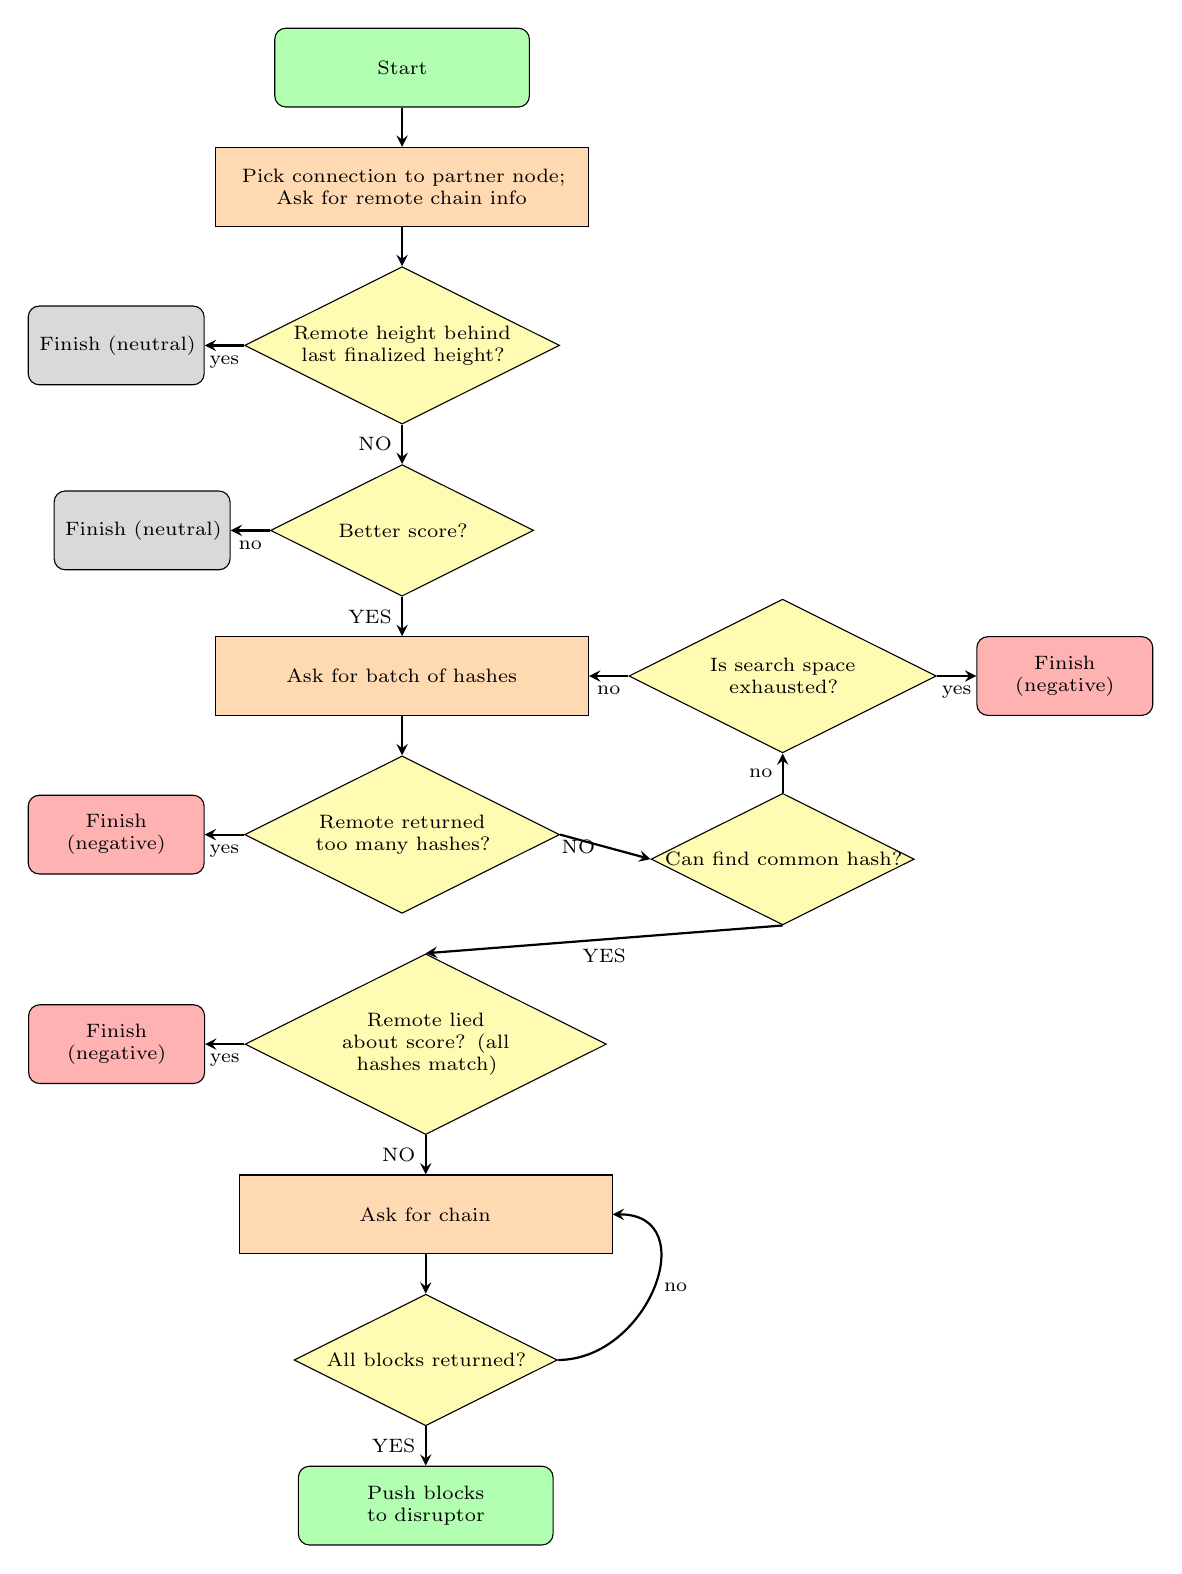
\begin{tikzpicture}[
	node distance=0.5cm and 0.5cm,
	font=\scriptsize
	]
\tikzset{
	base/.style = { rectangle, text centered, draw=black, minimum height=1cm },
	rounded/.style = { base, rounded corners },
	startfinish/.style = { rounded, fill=green!30, minimum width=2cm, text width=3cm },
	finishNeutral/.style = { rounded, fill=gray!30, minimum width=1.5cm, text width=2cm },
	finishNegative/.style = { rounded, fill=red!30, minimum width=1.5cm, text width=2cm },
	finishFailure/.style = { rounded, draw=black, fill=red!30, minimum width=1.5cm, text width=2cm },
	process/.style = { base, text width=4.5cm, fill=orange!30, minimum width=4cm },
	decision/.style = { diamond, text centered, draw=black, minimum height=1cm, aspect=2, text width=3cm, inner sep=0cm, fill=yellow!30, minimum width=2cm },
	arrow/.style ={ thick,->,>=stealth },
	line/.style = { thick,-,>=stealth },
	coord/.style={ coordinate },
	middleSpacing/.style = { xshift=0.3cm }
}

	% left column
	\node (start) [startfinish] {Start};
	\node (remoteScore) [process, below=of start] {Pick connection to partner node; \\ Ask for remote chain info};
	\node (decHeight) [decision, below=of remoteScore] {Remote height behind last finalized height?};
	\node (finishDecHeight) [finishNeutral, left=of decHeight] {Finish (neutral)};

	\node (decRemoteScore) [decision, below=of decHeight] {Better score?};
	\node (finishDecRemoteScore) [finishNeutral, left=of decRemoteScore] {Finish (neutral)};

	\node (remoteHashes) [process, below=of decRemoteScore] {Ask for batch of hashes};
	\node (decSearchSpace) [decision, right=of remoteHashes] {Is search space exhausted?};
	\node (finishDecSearchSpace) [finishNegative, right=of decSearchSpace] {Finish (negative)};

	\node (decHashesCount) [decision, below=of remoteHashes] {Remote returned too many hashes?};
	\node (finishDecHashesCount) [finishNegative, left=of decHashesCount] {Finish (negative)};
	\node (decHashesCommon) [decision, below=of decSearchSpace] {Can find common hash?};

	% right column
	\node (decHashesScoreLier) [decision, below=of decHashesCount, middleSpacing] {Remote lied about score? (all hashes match)};
	\node (finishDecHashesScoreLier) [finishNegative, left=of decHashesScoreLier] {Finish (negative)};

	\node (getBlocks) [process, below=of decHashesScoreLier] {Ask for chain};
	\node (decBlocksOk) [decision, below=of getBlocks] {All blocks returned?};

	\node (pushToDisruptor) [startfinish, below=of decBlocksOk] {Push blocks to disruptor};

	% paths
	\draw [arrow] (start) -- (remoteScore);
	\draw [arrow] (remoteScore) -- (decHeight);
	\draw [arrow] (decHeight) -- node[anchor=north] {\scriptsize{yes}} (finishDecHeight);
	\draw [arrow] (decHeight) -- node[anchor=east] {\scriptsize{NO}} (decRemoteScore);

	\draw [arrow] (decRemoteScore) -- node[anchor=north] {\scriptsize{no}} (finishDecRemoteScore);
	\draw [arrow] (decRemoteScore) -- node[anchor=east] {\scriptsize{YES}} (remoteHashes);

	\draw [arrow] (remoteHashes) -- (decHashesCount);
	\draw [arrow] (decHashesCount) -- node[anchor=north] {\scriptsize{yes}} (finishDecHashesCount);

	\draw [arrow] (decHashesCount.east) -- node[anchor=east] {\scriptsize{NO}} (decHashesCommon.west);

	\draw [arrow] (decSearchSpace)  -- node[anchor=north] {\scriptsize{no}} (remoteHashes.0);

	\draw [arrow] (decHashesCommon.south) -- node[anchor=north] {\scriptsize{YES}} (decHashesScoreLier.north);

	\draw [arrow] (decHashesScoreLier) -- node[anchor=north] {\scriptsize{yes}} (finishDecHashesScoreLier);
	\draw [arrow] (decHashesScoreLier) -- node[anchor=east] {\scriptsize{NO}} (getBlocks);

	\draw [arrow] (getBlocks) -- (decBlocksOk);
	\draw (decBlocksOk.0)  edge[arrow, out=0, in=0, looseness=1.5]  node[anchor=west] {\scriptsize{no}} (getBlocks.0);
	\draw [arrow] (decBlocksOk) -- node[anchor=east] {\scriptsize{YES}} (pushToDisruptor);

	\draw [arrow] (decHashesCommon) -- node[anchor=east] {\scriptsize{no}} (decSearchSpace);
	\draw [arrow] (decSearchSpace) -- node[anchor=north] {\scriptsize{yes}} (finishDecSearchSpace);
\end{tikzpicture}

		\caption{Blockchain synchronization flow chart\label{fig:blockchain:synchronizationFlowChart}}
	\end{center}
\end{figure}

\subsection{Blockchain Processing}

\subsubsection*{Execution}

Conceptually, when a new block is received, it is processed in a series of stages
\footnote{A more detailed description of these stages can be found in \nemref{sec:disruptor:consumers}.}.
Prior to processing, the block and its transactions are decomposed into an ordered stream of notifications.
A notification is the fundamental processing unit used in \codename.

In order to extract an ordered stream of notifications from a block, its transactions are decomposed in order followed by its block-level data.
The notifications produced by each decomposition are appended to the stream.
At the end of this process, the notification stream completely describes all state changes specified in the block and its transactions.

Once the stream of notifications is prepared, each notification is processed individually.
First, it is validated independent of blockchain state.
Next, it is validated against the current blockchain state.
If any validation fails, the containing block is rejected.
Otherwise, the changes specified by the notification are made to the in memory blockchain state and the next notification is processed.
This sequence allows transactions in a block to be dependent on changes made by previous transactions in the same block.

After all notifications produced by a block are processed, the \field{ReceiptsHash} \nemrefparens{sec:blocks:receiptshash} and \field{StateHash} \nemrefparens{sec:blocks:statehash} fields are calculated and checked for correctness.
Importantly, when \nemsetting{network}{enableVerifiableState} is enabled, this is the point at which all state patricia trees get updated.

\subsubsection*{Rollback}

Occasionally, a block that has been previously confirmed needs to be undone.
This is required in order to allow fork resolution.
For example, to replace a worse block with a better block.
In \codename, at most \nemsetting{network}{maxRollbackBlocks} can be rolled back at once.
Forks larger than this setting are irreconcilable.

When a block is being rolled back, it is decomposed into an ordered stream of notifications.
This stream is reversed relative to the stream used during execution.
Since transactions in a block may be dependent on changes made by previous transactions in the same block, they need to be undone before their dependencies are undone.

Once the stream of notifications is prepared, each notification is processed individually.
No validation is needed because the rollback operation is returning the blockchain to a previous state that is known to be valid.
Instead, the changes specified by the notification are simply reverted from the in memory blockchain state and the next notification is processed.

After all notifications produced by a \emph{blockchain part} are processed, the previous blockchain state is restored.
When \nemsetting{network}{enableVerifiableState} is enabled, the in memory state hash still needs to be updated.
Instead of individually applying all tree changes, the in memory state hash is forcibly reset to the state hash of the common block prior to the last rolled back block.

	\section{Disruptor}
\label{sec:disruptor}

\nemquote{%
Death is the great disruptor. It thrusts us opposite life's mirror, invites our truthful exploration, and reveals the naked truth from which rebirth is possible and we are free to reinvent ourselves anew.
}{B.G. Bowers}

\nemchapterfirstletter{O}{ne} main goal of \codenamespace is to achieve high throughput.
In order to help achieve this goal, the disruptor\footnote{ \url{https://en.wikipedia.org/wiki/Disruptor_(software)} } pattern is used to perform most data processing.
A disruptor uses a ring buffer data structure to hold all elements in need of processing.
New elements are inserted into the next free slot of the ring buffer.
Fully processed elements are removed to make space for new elements.
Since the ring buffer has a finite number of slots, it can run out of space if processing can't keep up with new insertions.
The behavior of \codename, in such a case, can be configured to either exit the server or discard new data until a slot becomes available.

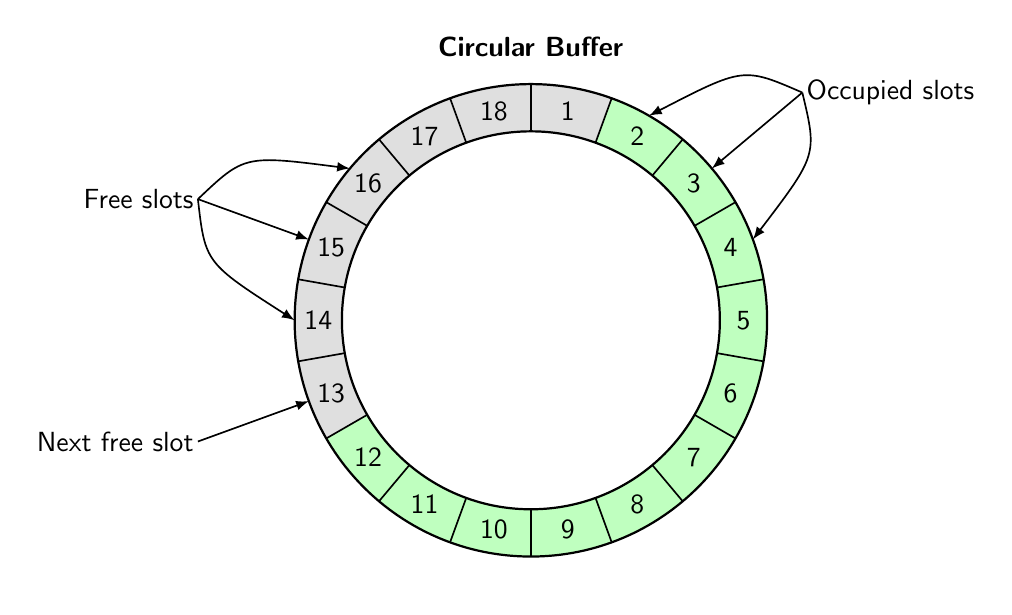
\begin{tikzpicture}[>=latex,font=\sffamily,semithick,scale=3,label distance=-2mm]
	\fill [green!25] (0,0) -- (70:1) arc [end angle=-150, start angle=70, radius=1] -- cycle;
	\fill [gray!25] (0,0) -- (70:1) arc [end angle=210, start angle=70, radius=1] -- cycle;
	\draw [thick,minimum size=6cm] (0,0) circle(1);
	\draw (90:1.1) node[label=above:\textbf{Circular Buffer}]{};
	\foreach \angle in {90,70,...,-70}
		\draw (\angle:1) -- (\angle-180:1);

	\foreach \angle [count=\anglei] in {80,60,...,-260}
		\draw (\angle:0.9) node[] {\anglei};

	\draw [thick,fill=white,minimum size=3cm] (0,0) circle(0.8);

	\draw [->] (160:1.5) .. controls (170:1.4) .. (180:1);
	\draw [->] (160:1.5) -- (160:1);
	\draw [->] (160:1.5) .. controls (150:1.4) .. (140:1);
	\draw [] (160:1.5) node[label=left:Free slots]{};

	\draw [->] (40:1.5) .. controls (50:1.4) .. (60:1);
	\draw [->] (40:1.5) -- (40:1);
	\draw [->] (40:1.5) .. controls (30:1.4) .. (20:1);
	\draw [] (40:1.5) node[label=right:Occupied slots]{};

	\draw [->] (200:1.5) -- (200:1);
	\draw (200:1.5) node[label=left:Next free slot]{};

	(Head.west);
\end{tikzpicture}

Each element in the ring buffer is processed by one or more consumers.
Each consumer takes a single element as input.
Some consumers calculate data from the input and attach it to the element, while others validate the element or alter the global chain state using the element's data.
Some consumers depend on the work done by previous consumers.
Therefore, consumers always need to act on input elements in a predefined order.
To ensure this, each consumer has an associated barrier.
The barrier prevents a consumer from processing an element that has not yet been processed by its immediately preceding consumer.
The last consumer reclaims all memory that was used during processing.
Consumers can set an element's completion status to \structField{CompletionStatus}{Aborted} in case it is already known or invalid for some reason.
Subsequent consumers ignore aborted elements.

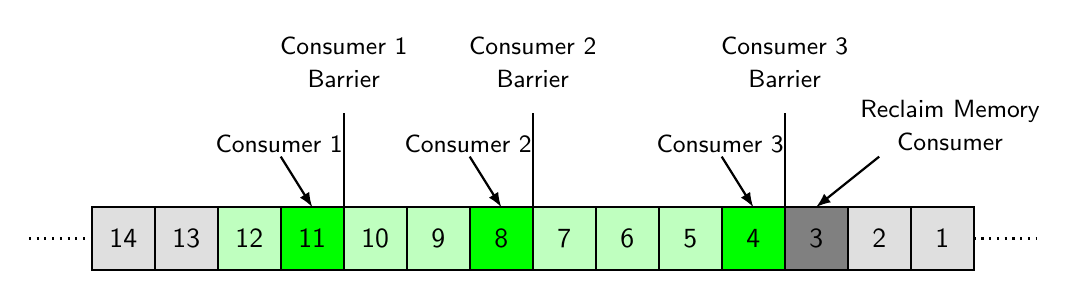
\begin{tikzpicture}[>=latex,font=\sffamily,thick,,scale=0.8]
	% Dots
	\draw[thick,dotted,step=.5] (0,0.5) grid (1,0.5);
	\draw[thick,dotted,step=.5] (15,0.5) grid (16,0.5);

	% Rectangles
	\foreach \i [] in {1,2,13,14}
		\filldraw[draw=black,fill=gray!25] (\i,0) rectangle (\i+1,1);
	\foreach \i [] in {3,5,6,8,9,10}
		\filldraw[draw=black,fill=green!25] (\i,0) rectangle (\i+1,1);
	\foreach \i [] in {4,7,11}
		\filldraw[draw=black,fill=green] (\i,0) rectangle (\i+1,1);
	\filldraw[draw=black,fill=gray] (12,0) rectangle (13,1);

	% Consumer 1
	\draw [] (5,2.0) node[xshift=0.25cm,label=left:\small{Consumer 1}]{};
	\draw [->] (4,1.8) -- (4.5,1);
	\draw [] (5,3.3) node[align=center]{\small{Consumer 1}\\\small{Barrier}};
	\draw [] (5,1) -- (5, 2.5);

	% Consumer 2
	\draw [] (8,2.0) node[xshift=0.25cm,label=left:\small{Consumer 2}]{};
	\draw [->] (7,1.8) -- (7.5,1);
	\draw [] (8,3.3) node[align=center]{\small{Consumer 2}\\\small{Barrier}};
	\draw [] (8,1) -- (8, 2.5);

	% Consumer 3
	\draw [] (12,2.0) node[xshift=0.25cm,label=left:\small{Consumer 3}]{};
	\draw [->] (11,1.8) -- (11.5,1);
	\draw [] (12,3.3) node[align=center]{\small{Consumer 3}\\\small{Barrier}};
	\draw [] (12,1) -- (12, 2.5);

	% Reclaim memory consumer
	\draw [] (13,2.3) node[align=center,xshift=1.3cm]{\small{Reclaim Memory}\\\small{Consumer}};
	\draw [->] (13.5,1.8) -- (12.5,1);

	% Numbers
	\foreach \index [count=\indexi] in {14,13,...,1}
	\draw (\indexi+0.5,0.5) node[] {\index};
\end{tikzpicture}

\subsection{Consumers}
\index{consumers}
\label{sec:disruptor:consumers}
In \codename, a block disruptor is used to process incoming blocks and blockchain parts.
A blockchain part is an input element composed of multiple blocks.
This disruptor is primarily responsible for validating, reconciling and growing the blockchain.

A transaction disruptor is used to process incoming, unconfirmed transactions.
Transactions that are fully processed get added to the unconfirmed transactions cache.

All disruptors are associated with a chain of consumers that perform all processing of their input elements.
Different disruptors are customized by using different consumer chains.
All consumers can inspect the data being processed and some can modify it.

\begin{figure}[H]
	\nemcenterwithcaption{
		\begin{subfigure}{.5\textwidth}
			\nemcenterwithcaption{
				\tikzstyle{consumer} = [rectangle, rounded corners, text centered, draw=black, minimum width=7cm, minimum height=0.5cm, text width=6.5cm]
				\vspace{0pt}
				\begin{tikzpicture}[>=latex,font=\small ,semithick,scale=1,node distance=1.1cm]
					% block consumers
					\node (audit consumer) [consumer] {Audit Consumer (optional)};
					\node (hash calculator consumer) [consumer, below of=audit consumer] {Hash Calculator Consumer};
					\node (hash check consumer) [consumer, below of=hash calculator consumer] {Hash Check Consumer};
					\node (blockchain check consumer) [consumer, below of=hash check consumer] {Blockchain Check Consumer};
					\node (stateless validation consumer) [consumer, below of=blockchain check consumer] {Stateless Validation Consumer};
					\node (batch signature consumer) [consumer, below of=stateless validation consumer] {Batch Signature Consumer};
					\node (blockchain sync consumer) [consumer, below of=batch signature consumer] {Blockchain Sync Consumer};
					\node (blockchain sync cleanup consumer) [consumer, below of=blockchain sync consumer] {Blockchain Sync Cleanup Consumer (optional)};
					\node (new block consumer) [consumer, below of=blockchain sync cleanup consumer] {New Block Consumer};

					% arrows
					\draw [semithick,->] (audit consumer) -- (hash calculator consumer);
					\draw [semithick,->] (hash calculator consumer) -- (hash check consumer);
					\draw [semithick,->] (hash check consumer) -- (blockchain check consumer);
					\draw [semithick,->] (blockchain check consumer) -- (stateless validation consumer);
					\draw [semithick,->] (stateless validation consumer) -- (batch signature consumer);
					\draw [semithick,->] (batch signature consumer) -- (blockchain sync consumer);
					\draw [semithick,->] (blockchain sync consumer) -- (blockchain sync cleanup consumer);
					\draw [semithick,->] (blockchain sync cleanup consumer) -- (new block consumer);
				\end{tikzpicture}
			}{Block Consumers}
		\end{subfigure}%
		\begin{subfigure}{.5\textwidth}
			\nemcenterwithcaption{
				\tikzstyle{consumer} = [rectangle, rounded corners, text centered, draw=black, minimum width=6cm, minimum height=0.6cm, text width=6.5cm]
				\vspace{0pt}
				\begin{tikzpicture}[>=latex,font=\small,semithick,scale=1,node distance=1.1cm]
					% transactions consumers
					\node (audit consumer) [consumer] {Audit Consumer (optional)};
					\node (hash calculator consumer) [consumer, below of=audit consumer] {Hash Calculator Consumer};
					\node (hash check consumer) [consumer, below of=hash calculator consumer] {Hash Check Consumer};
					\node (dummy1) [consumer, below of=hash check consumer, draw=none] {};
					\node (stateless validation consumer) [consumer, below of=dummy1] {Stateless Validation Consumer};
					\node (batch signature consumer) [consumer, below of=stateless validation consumer] {Batch Signature Consumer};
					\node (dummy2) [consumer, below of=batch signature consumer, draw=none] {};
					\node (dummy3) [consumer, below of=dummy2, draw=none] {};
					\node (new transactions consumer) [consumer, below of=dummy3] {New Transactions Consumer};

					% arrows
					\draw [semithick,->] (audit consumer) -- (hash calculator consumer);
					\draw [semithick,->] (hash calculator consumer) -- (hash check consumer);
					\draw [semithick,->] (hash check consumer) -- (stateless validation consumer);
					\draw [semithick,->] (stateless validation consumer) -- (batch signature consumer);
					\draw [semithick,->] (batch signature consumer) -- (new transactions consumer);
				\end{tikzpicture}
			}{Transactions Consumers}
		\end{subfigure}
	}{\codenamespace consumer chains}
\end{figure}

\subsubsection{Common Consumers}
\label{sec:disruptor:commonConsumers}
\index{consumers!common}
The block and transaction disruptors share a number of consumers.

\subsubsection*{Audit Consumer}
This consumer is optional and can be enabled via node configuration.
If enabled, all new elements are written to disk.
This makes it possible to replay the incoming network action and is helpful for debugging.

\subsubsection*{Hash Calculator And Hash Check Consumers}
It is very common for a server to receive the same element many times because networks consist of many servers that broadcast elements to several other servers.
For performance reasons, it is desirable to detect at an early stage whether an element has already been processed in order to avoid processing it again.

The hash calculator consumer calculates all the hashes associated with an element.
The hash check consumer uses the hashes to search the recency cache, which contains the hashes of all recently seen elements.
The consumer used by the transaction disruptor will also search the hash cache (containing hashes of confirmed transactions) and the unconfirmed transactions cache.
If the hash is found in any cache, the element is marked as \structField{CompletionStatus}{Aborted} and further processing is bypassed.

\subsubsection*{Stateless Validation Consumer}
This consumer handles state independent validation by validating each entity in an element.
This can be done in parallel using many threads.
Each plugin can add stateless validators.

An example of a stateless validation is the validation that a block does not contain more transactions than allowed by the network.
This check depends on the network configuration but not on the global blockchain state.

\subsubsection*{Batch Signature Consumer}
This consumer validates all signatures of all entities in an element.
This is separate from the \emph{Stateless Validation Consumer} because it uses batch verification.
For improved performance, this consumer processes many signatures at once in a batch instead of individually.
This can be done in parallel using many threads.

\subsubsection*{Reclaim Memory Consumer}
This consumer completes the processing of an element and frees all memory associated with it.
It triggers downstream propagation of the statuses of all transactions that were updated during processing.
The overall result of the sync operation is used to update the reputation of - and possibly ban - the sync partner \nemrefparens{sec:reputation}).

\subsubsection{Additional Block Consumers}
\label{sec:disruptor:blockConsumers}
\index{consumers!block}
The block disruptor also uses a few block-specific consumers.

\subsubsection*{Blockchain Check Consumer}
This consumer performs state-independent integrity checks of the chain part contained within an element.
It checks that:
\begin{itemize}
	\item{The chain part is not composed of too many blocks.}
	\item{The timestamp of the last block in the chain part is not too far in the future.}
	\item{All blocks within the chain part are linked.}
	\item{There are no duplicate transactions within the chain part.}
\end{itemize}

\subsubsection*{Blockchain Sync Consumer}
This consumer is the most complex one.
All tasks that require or alter the local server's chain state are performed in this consumer.

First, it checks that the new chain part can be attached to the existing chain.
If the chain part attaches to a block preceding the tail block, all blocks starting with the tail block are undone in reverse order until the common block is reached.

Next, it executes each block by performing stateful validation and then observing changes.
Stateless validation is skipped because it was performed by previous consumers.
If there are any validation failures, the entire chain part is rejected.
Otherwise, all changes are committed to the chain state (both the block and cache storages) and the unconfirmed transactions cache is updated.

\emph{This consumer is the only part of the \codenamespace system that modifies the chain state and needs write access to it.}

\subsubsection*{Blockchain Sync Cleanup Consumer}
This consumer is optional and can be enabled via node configuration.
If enabled, it removes all files that were created by the \emph{Blockchain Sync Consumer}.
This consumer should only be enabled when a server is running without a broker.

\subsubsection*{New Block Consumer}
This consumer forwards single blocks, either harvested by the server or pushed from a remote server, to other servers in the network.

\subsubsection{Additional Transaction Consumers}
\label{sec:disruptor:transactionConsumers}
\index{consumers!transaction}
The transaction disruptor uses a single transaction-specific consumer.

\subsubsection*{New Transactions Consumer}
This consumer forwards all transactions that have valid signatures and have passed stateless validation to the network.
Stateful validation is not performed on transactions until they're added to the unconfirmed transactions cache.
Forwarding is intentionally done before stateful validation because one server might reject transactions that could be accepted by other servers (e.g. if the transaction has too low a fee for the local server).
Subsequently, stateful validation is performed on the forwarded transactions, and the valid ones are stored in the unconfirmed transactions cache.

	\section{Unconfirmed Transactions}
\label{sec:unconfirmedTransactions}

\nemquote{%
I don’t believe one reads to escape reality.
A person reads to confirm a reality he knows is there, but which he has not experienced.
}{Lawrence Durrell}

\nemchapterfirstletter{A}{ny} transaction that is not yet included in a block is called an \emph{unconfirmed transaction}.
These transactions may be valid or invalid.
Valid unconfirmed transactions are eligible for inclusion in a harvested block.
Once a transaction is added to a block that is accepted in the blockchain, it is \emph{confirmed}.

Unconfirmed transactions can arrive at a node when:
\begin{enumerate}
	\item{A client sends a new transaction directly to the node.}
	\item{A bonded aggregate transaction is completed with all requisite cosignatures and is promoted from the partial transactions cache.}
	\item{A Peer node broadcasts transactions to the node.}
	\item{
		A Peer node responds to the node's request for unconfirmed transactions.
		As an optimization, the requesting node indicates what transactions it already knows in order to avoid receiving redundant transactions.
		Additionally, it supplies the minimum fee multiplier \nemrefparens{sec:blockchain:generation} it uses when creating blocks.
		This prevents the remote node from returning unconfirmed transactions that will be immediately rejected by the requesting node.
	}
\end{enumerate}

When an unconfirmed transaction arrives at a node, it is added to the transaction disruptor \nemrefparens{sec:disruptor}.
All transactions that haven't been previously seen and pass stateless validation will be broadcast to peer nodes.
At this point, it is still possible for the node to reject the broadcast transactions because stateful validation is performed after broadcasting.
Due to different node settings, it's possible for some nodes to accept a specific unconfirmed transaction and other nodes to reject it.
For example, the nodes could have different \nemsetting{node}{minFeeMultiplier} settings.

\subsection{Unconfirmed Transactions Cache}
\index{unconfirmed transactions!cache}

When a transaction passes all validation, it is eligible for inclusion in a harvested block.
At this point, the node tries to add it to the \emph{unconfirmed transactions cache}.
This can fail for two reasons:
\begin{enumerate}
	\item{The maximum cache size configured by \nemsetting{node}{unconfirmedTransactionsCacheMaxSize} has been reached.}
	\item{The cache contains at least as many unconfirmed transactions as can be included in a single block and the new transaction is rejected by the Spam throttle.}
\end{enumerate}

Whenever new blocks are added to the blockchain, the blockchain state changes and the unconfirmed transactions cache is affected.
Although all transactions in the cache are valid at the time they were added, this doesn't guarantee that they'll be valid in perpetuity.
For example, a transaction could have already been included in a block harvested by another node or a conflicting transaction could have been added to the blockchain.
This means that transactions in the cache that were perfectly valid previously could be invalidated after changes to the blockchain state.
Additionally, when blocks with transactions are reverted, it's possible that some of those previously confirmed transactions are no longer included in any block in the new chain.
Those reverted transactions should be added to the cache.

As a result of these considerations, the entire unconfirmed transactions cache is completely rebuilt whenever the blockchain changes.
Each transaction is rechecked by the stateful validators and purged if it has become invalid or has already been included in a block.
Otherwise, it is added back to the cache.

\subsection{Spam Throttle}
\index{unconfirmed transactions!spam throttle}

The initiator of an unconfirmed transaction does not have to pay a fee to nodes holding the transaction in the unconfirmed transactions cache.
Since the cache uses valuable resources, a node must have some protection against being spammed with lots of unconfirmed transactions.
This is especially important if the node is generous and accepts zero fee transactions.

Simply limiting the number of unconfirmed transactions that a node accepts is suboptimal because normal actors should still be able to send a transaction even when a malicious actor is spamming the network.
Limiting the number of unconfirmed transactions per account is also not a good option because accounts are free to create.

\codenamespace implements a smart throttle that prevents an attacker from filling the cache completely with transactions while still letting honest actors successfully submit new unconfirmed transactions.
\nemsetting{node}{enableTransactionSpamThrottling} can be used to activate the throttle.
Assuming the cache is not full, it works in the following way:
\begin{enumerate}
	\item{If the cache contains fewer unconfirmed transactions than can be included in a single block, throttling is bypassed.}
	\item{If the new transaction is a bonded aggregate transaction, throttling is bypassed.}
	\item{Else the Spam throttle is applied.}
\end{enumerate}

Let $\mathvar{curSize}$ be the current number of transactions in the cache and $\mathvar{maxSize}$ the configured maximum size of the cache.
Also let $\mathname{rel. importance of A}$ be the relative importance of $A$, i.e. a number between 0 and 1.
If a new unconfirmed transaction $T$ with signer $A$ arrives, then the $\mathname{fair share}$ for account $A$ is calculated:
\begin{align*}
	\mathvar{maxBoostFee} &= \nemsetting{node}{transactionSpamThrottlingMaxBoostFee} \\
	\mathvar{maxFee} &= \min(\mathvar{maxBoostFee}, \structField{T}{MaxFee}) \\
	\mathname{eff. importance} &= (\mathname{rel. importance of A}) + 0.01 \cdot \frac{\mathvar{maxFee}}{\mathvar{maxBoostFee}} \\
	\mathname{fair share} &= 100 \cdot (\mathname{eff. importance}) \cdot (\mathvar{maxSize} - \mathvar{curSize}) \cdot \exp\left(-3 \frac{\mathvar{curSize}}{\mathvar{maxSize}}\right)
\end{align*}

If account $A$ already has as many transactions in the cache as its fair share, then the new transaction is rejected.
Otherwise, it is accepted.
The formula shows that an increase in a transaction's maximum fee increases the number of slots available in the cache.
Nonetheless, this mechanism for boosting the effective importance is limited by \nemsetting{node}{transactionSpamThrottlingMaxBoostFee}.

\begin{figure}[ht]
	\nemcenterwithcaption{
		\pgfplotsset{
			legend entry/.initial=,
			every axis plot post/.code={%
				\pgfkeysgetvalue{/pgfplots/legend entry}\tempValue
				\ifx\tempValue\empty
					\pgfkeysalso{/pgfplots/forget plot}%
				\else
					\expandafter\addlegendentry\expandafter{\tempValue}%
				\fi
			},
		}
		\begin{tikzpicture}[trim axis left]
			\begin{axis}[
					scale only axis,
					xlabel = \text{cache fill level [\%]},
					xticklabel={\pgfmathparse{int(\tick / 100)}\pgfmathprintnumber{\pgfmathresult}},
					scaled x ticks=false,
					ylabel = fair share,
					height = 5cm,
					width=(4 * \textwidth) / 5
				]
				\addplot[color=blue,domain=1500:10000,legend entry=$0.01\%$]{100 * 0.0001 * (10000 - x) * exp(-3 * x / 10000)};
				\addplot[color=red,domain=1500:10000,legend entry=$0.005\%$]{100 * 0.00005 * (10000 - x) * exp(-3 * x / 10000)};
				\addplot[color=green,domain=1500:10000,legend entry=$0.001\%$]{100 * 0.00001 * (10000 - x) * exp(-3 * x / 10000)};
			\end{axis}
		\end{tikzpicture}
	}{Fair share for various effective importances with max cache size = 10000}
	\label{fig:unconfirmedTransactions:fairShare}
\end{figure}

\autoref{fig:unconfirmedTransactions:fairShare} shows the fair share of slots relative to the fill level of the cache for various effective importances.
An attacker that tries to occupy many slots cannot gain much by using many accounts because the importance of each account will be very low.
The attacker can increase maximum transaction fees but that will be more costly and expend funds at a faster rate.

	\include{chapters/partial}
	\section{Network}
\label{sec:network}

\nemquote{%
Pulling a good network together takes effort, sincerity and time.
}{Alan Collins}

\nemchapterfirstletter{D}{ynamic} discovery of nodes\index{node} allows a peer-to-peer network to grow.
\codenamespace implements this dynamic discovery in the \emph{node discovery extension}.
Public networks are typically open and allow any node to join.
Private networks can restrict the nodes that are allowed to join and behave as a federated system
\footnote{
	By carefully distributing harvesting and currency mosaics, a private network can delegate permissions to different accounts.
	For example, only accounts owning sufficient harvesting mosaic can create blocks and only accounts with nonzero currency can initiate transactions with nonzero fees.
}.
\codenamespace is flexible enough to even allow private networks to specify all node relationships via configuration files.

\codenamespace supports a configurable node identification policy configured by \nemsetting{network}{nodeEqualityStrategy}.
Valid policies allow identifying a node by either its \emph{resolved IP} (\texttt{host})
\footnote{
	A node's resolved IP is only broadcast to other nodes when it doesn't specify a hostname.
	Hostnames are preferentially propagated in order to support nodes with dynamic IPs.
} or \emph{public boot key} (\texttt{public-key}).
The former is preferred for public networks.

\subsection{Beacon Nodes}

A freshly booted node is initially isolated and not connected with any peers.
It needs to join a network before it can make any meaningful contributions, like validating or harvesting blocks.
In \codename, a list of \emph{static}\index{node!static} beacon nodes are stored in a peers configuration file.
In order to join a network, a new node first connects to these nodes.
These files don't need to be identical across all nodes in a network.

A public network is recommended to specify a set of high availability beacon node candidates.
Each node's peers configuration file should contain a random subset of these nodes.
The random subset can be selected once before connecting to the network for the first time or more frequently before every boot.
The important thing is that beacon nodes are well distributed.
This reduces stress on individual beacon nodes and makes DoS attacks on beacon nodes more difficult.
These nodes are given slight preference in node selection \nemrefparens{sec:reputation:NodeSelection} relative to non-beacon nodes because they are assumed to have high-availability.
They aren't conferred any other special privileges or responsibilities.
They can be thought of as doors into the network.

Certain extensions may require their own set of beacon nodes.
For example, the \emph{partial transaction extension} stores its own set of beacon nodes in a separate peers configuration file.
Nodes with this extension enabled need to additionally synchronize partial transactions among other nodes that also have this extension enabled  \nemrefparens{sec:partials}.

A node's roles specify the capabilities it supports.
Typically, these are used by a connecting node to choose appropriate partners.
Nodes with the \texttt{Peer} role support basic synchronization.
Nodes with the \texttt{API} role support partial transaction synchronization.
Nodes with the \texttt{Voting} role participate in the finalization voting procedure when deterministic finalization is enabled.
Nodes with the \texttt{IPv4} role support IPv4 communication.
Nodes with the \texttt{IPv6} role support IPv6 communication\footnote{
	If a node does not explicitly specify an \texttt{IPv4} and/or \texttt{IPv6} role, it is assumed to support \texttt{IPv4} communication only.
}.
Roles are not mutually exclusive.
Nodes are allowed to support multiple roles.

\subsection{Connection Handshake}
\label{sec:network:connectionHandshake}
\index{TLS}

All connections among \codenamespace nodes are made over TLS v1.3 with a custom verification procedure.
Each node is expected to have a two level deep X509 certificate chain composed of a \emph{root} certificate and a \emph{node} certificate.
All certificates must be X25519 certificates.
\codenamespace doesn't support any other certificate types.

The root certificate is expected to be self-signed with an account's \emph{signing private key}.
This account is assumed to be a node's unique owner.
Cryptographically linking a node and an account allows selection algorithms to perform node weighting based on the node owner's importance.
Additionally, partner nodes use this verified identity to collate reputation \nemrefparens{sec:reputation} information\footnote{
	In the public network, nodes are primarily identified by their resolved IP.
}.
Importantly, this certificate is only used for signing the node certificate.
For security, its private key should not be kept on a running server.

The node certificate is signed by the root certificate.
It can contain a random public/private key pair.
This certificate is used for authenticating TLS sessions and deriving shared encryption keys for encrypting optional data\footnote{
	Currently, the only encryption key derived is the one used to encrypt and decrypt messages related to automatic delegated harvester detection
	\nemrefparens{sec:blockchain:delegatedHarvesterDetection}.
}.
It can be rotated as often as desired.

This authentication procedure is performed independently by each partner node.
If either node fails the handshake, the connection is immediately terminated.

\subsection{Packets}

\codenamespace uses TCP for network communication on the port specified by \nemsetting{node}{port}.
Communication is centered around a higher level \emph{packet} model on top of and distinct from TCP packets.
All packets begin with an 8-byte header that specifies each packet's size and type.
Once a complete packet is received, it is ready for further processing.

\begin{figure}[H]
	\nemcenter{
		\nemmemorylayout{
				\begin{leftwordgroup}{\texttt{0x00}}
					\bitbox{4}{Size} \bitbox{4}{Type}
				\end{leftwordgroup}
		}{Packet header binary layout}
	}{}
\end{figure}

A mix of long lived and short lived connections are used.
Long lived connections are used for repetitive activities like syncing blocks or transactions.
They support both push and request/response semantics.
The connections are allowed to last for \nemsetting{node}{maxConnectionAge} selection rounds \nemrefparens{sec:reputation:ConnectionManagement} before they are eligible for recycling.
Connections older than this setting are recycled primarily to allow direct interactions with other partner nodes and secondarily as a precaution against zombie connections.

Short lived connections are used for more complex multistage interactions between nodes.
For example, they are used for node discovery \nemrefparens{sec:network:discovery} and time synchronization \nemrefparens{sec:timesync}.
Short lived connections help prevent sync starvation, which can occur when all long lived connections are in use and no sync partners are available.

\emph{Handlers} are used to process packets.
Each handler is registered to accept all packets with a specified packet type.
When a complete packet is ready for processing, it is dispatched to the handler registered with its type.
All handlers must accept matching packets for processing.
Some handlers can also write response packets in order to allow request/response protocols.

\subsection{Connection Types}

In \codename, long lived connections are primarily identified as readers or writers.
This is orthogonal to whether they are incoming or outgoing.
They are secondarily identified by purpose, or \emph{service identifier}
\footnote{Although the terminology is similar, these are unrelated to services described in \nemref{sec:system:extensions}.}.
This allows connections to be selected by capability and more granular logging.

Reader connections are mostly passive and used to receive data from other nodes.
Each server asynchronously reads from each reader connection.
Whenever a new packet is received in its entirety, it is dispatched to an appropriate handler.
If no matching handler is available, the connection is closed immediately.

The \nemsetting{node}{maxIncomingConnectionsPerIdentity} limit is applied across all services and long and short lived connections.
Any incoming connections above this limit will be immediately closed.
This limit can be hit when multiple short lived connections are initiated with the same remote node for different operations.
This is more likely when connection tasks are more aggressively scheduled immediately after a node boots up.
These errors are typically transient and can be safely ignored if they don't persist.

Writer connections are more active and used to send data to other nodes.
\emph{Broadcast} operations push data to all active and available writers.
Additionally, writers can be selected individually and used for request/response protocols.
In order to simplify recipient processing, writers participating in an ongoing request/response protocol are not sent broadcast packets.

Service identifiers are only assigned to long lived connections.
Sync service is used to manage outgoing connections to nodes with \texttt{Peer} role.
API partial service is used to manage outgoing connections to nodes with \texttt{API} role.
Readers service is used to manage incoming connections.
API writers service is experimental and allows incoming connections on port \nemsetting{node}{apiPort} to register as writers.

\begin{figure}[H]
	\nemcenterwithcaption{
		\begin{tabular}{|c|c|c|}
			\hline
			Identifier & Name & Direction\\
			\hline
			0x50415254 & pt.writers & outgoing \\
			0x52454144 & readers & incoming \\
			0x53594E43 & sync & outgoing \\
			\hline
		\end{tabular}
	}{Service Identifiers}
	\label{tbl:network:serviceIdentifiers}
\end{figure}

For the purposes of node selection described in \nemref{sec:reputation:NodeSelection}, node aging and selection are both scoped per service.
Reputational information is aggregated across all services.
Specifically, assume a node has made both a Sync and API partial connection to another node.
Each connection can have a different age because age is scoped per service.
Interaction results, from any connection, are always attributed to the node, not the service.

\subsection{Peer Provenance}

A node collects data about all nodes in its network.
The reputability of the data is dependent on its provenance.
Possible provenances, ranked from best to worst are:
\begin{enumerate}
	\item{Local - Node is specified in \nemsetting{node}{localnode}.}
	\item{Static - Node is in one of the peers configuration files.}
	\item{Dynamic - Node was discovered and supports connections.}
	\item{Dynamic Incoming - Node has made a connection but does not support connections.}
\end{enumerate}

It is important to note that the distinguishing characteristic of a \emph{static} node is that it is listed in at least one local peers configuration file.
For emphasis, it is possible for one partner to view a node as static while another partner views it as dynamic.
Excepting the \emph{local} node, all other nodes are \emph{dynamic}\index{node!dynamic}.
A subset of dynamic nodes are \emph{incoming}.
These nodes have only been seen in incoming but not outgoing connections.
As a result, their preferred port is unknown and they can't be connected with.

Existing node data can only be updated if the new data does not have worse provenance than the existing data.
For example, updated information about a static node with dynamic provenance is discarded, but updated information about a dynamic node with dynamic or static provenance is allowed.

The above is a slight simplification due to how connections are actually managed.
When a node disconnects completely from a remote node and reconnects, the update can be a two step process.
Consider a dynamic node that attempts to reconnect to a remote with a different identity public key.
When the node initiates a connection, the remote will classify the connection as dynamic incoming, which has a worse provenance than dynamic.
As a result, the remote will not update the node's information.
Instead, it will set a flag indicating a possible identity update in progress.
Later on, when the remote directly connects to the node, it will get the same updated information as before.
At this point, the remote will update the information even though an active (dynamic incoming) connection is present because an in progress identity update was detected previously.
Without this flag, the active connection with worse provenance would block updates, which is undesirable.

When \nemsetting{network}{nodeEqualityStrategy} is \texttt{public-key}, the secondary identity component is the resolved IP.
When there are no active connections, this is allowed to change.
This strategy does not support reputational migration.

When \nemsetting{network}{nodeEqualityStrategy} is \texttt{host}, the secondary identity component is the node identity public key.
When there are no active connections, this is allowed to change.
The resolved IP primary identity component can also be changed when there are no active connections assuming the secondary identity component is unchanged.
In this case, all reputation data associated with the original host is migrated to the new host.
When there is an ambiguous match, data with the matching primary identity component is migrated and data with the matching secondary identity component is discarded.

\subsection{Node Discovery}
\label{sec:network:discovery}

After starting up, a node attempts to make short lived connections to all static nodes it has loaded from its peers configuration files.
These connections are primarily intended to retrieve the resolved IP addresses of all static nodes.
This allows hostnames to be used in the peers configuration files and simplifies node management.
As long as the node is running, this procedure is periodically repeated with a linear backoff.

Periodically, a node will broadcast identifying information about itself to its remote partner nodes.
The remote will process the received payload and check it for validity and compatibility.
In order to be valid, the identity public key specified by the node must match the public key of its root X509 certificate.
In order to be compatible, both the broadcasting and receiving nodes must target the same network.
If no hostname is provided, the node's resolved IP will be used in place.
If all checks succeed, the node will be added as a new potential partner and will be eligible for selection in the next sync round.

Periodically, a node will request all known peers from its remote partner nodes.
The remote nodes will respond with all of their active static and dynamic peers.
To the requesting node, these will all be treated as dynamic nodes.
The original node will request the identifying information from each of these nodes directly.
This direct communication is required to prevent a malicious actor from relaying false information about other nodes and to ensure a connection can be established with each new node.
The original node will process the received payload and check it for validity and compatibility as above.
If all checks succeed, the new node will be added as a new potential partner and will be eligible for selection in the next sync round.

	\section{Reputation}
\label{sec:reputation}

\nemquote{%
It takes many good deeds to build a good reputation, and only one bad one to lose it.
}{Benjamin Franklin}

\codenamechapterfirstword uses a peer-to-peer (P2P) network.
P2P networks have the great advantage of being robust because they cannot be shut down by eliminating a single node.
Nevertheless, a public network comes with its own challenges.
The participants of the network are anonymous and anyone can join.
This makes it very easy to inject hostile nodes into the network that spread invalid information or try to disturb the network in some way.

There is a need to identify hostile nodes and reduce communication with them.
There have been many approaches to achieve this.
One of the most successful is building a reputation system for nodes.
\codenamespace follows this approach by implementing a simple reputation system.
This system attempts to prioritize connections to well-behaved nodes over those to misbehaving nodes.
Importantly, reputation doesn't affect the blockchain consensus at all.
It only influences the network graph.
This chapter will outline the heuristics used.

\subsection{Connection Management}
\index{reputation!connection management}
\label{sec:reputation:ConnectionManagement}

Each node can establish at most \nemsetting{node}{maxConnections} persistent connections at once.
This limit is expected to be much smaller than the hundreds of thousands of nodes that make up the network as a whole.
In order to avoid isolated node groups from forming, a node will periodically drop existing connections to make room for new connections to different nodes.

When determining the nodes from which to disconnect, a node inspects the ages of all of its connections.
In order to minimize connection overhead, only connections that have been established for at least \nemsetting{node}{maxConnectionAge} rounds are eligible for removal.
The next time a node selection round is done, these connections are dropped and replaced with new connections to other nodes.
This guarantees that over time each node will make connections to many different nodes in the network.

\subsection{Weight Based Node Selection}
\index{node!selection}
\index{reputation!node selection|see {node, selection}}
\label{sec:reputation:NodeSelection}

Nodes primarily communicate with each other via the current persistent connections they have established.
A node can query another node for new transactions or blocks, or ask for a list of other nodes with which the partner node has interacted.
Nodes can also voluntarily send data to other nodes.
Each communication between nodes is considered an interaction and each interaction is scored as either successful, neutral or failed.
For example, when a remote node sends new valid data, the interaction is considered successful because it has contributed to the synchronization of the two nodes.
If the remote node has no new data, the interaction is neutral.
Otherwise, the interaction is considered failed.

Each node keeps track of the outcomes of its own interactions with other nodes.
These outcomes are only used locally and not shared with other nodes.
A node's interactions with other nodes influence the partner nodes it selects.
Interaction results are stored for at most one week but reset on node restart.
These results are time-limited to allow nodes that are having transient failures to reestablish themselves as good partners.

When selecting partner nodes, a node first determines a set of candidate nodes.
Each candidate node is assigned a raw weight between 500 and 10000 according to the following criteria:

\begin{itemize}
	\item{
		If there were 3 or fewer non-neutral interactions with the remote node, it is given a medium raw weight of 5000.
		This gives new nodes a good chance of getting selected.
	}
	\item{
		Else let $s$ be the number of successful and $f$ the number of failed interactions.
		Then the raw weight is calculated by the following formula:

		\begin{figure}[t!]
			\nemcenterwithcaption{
				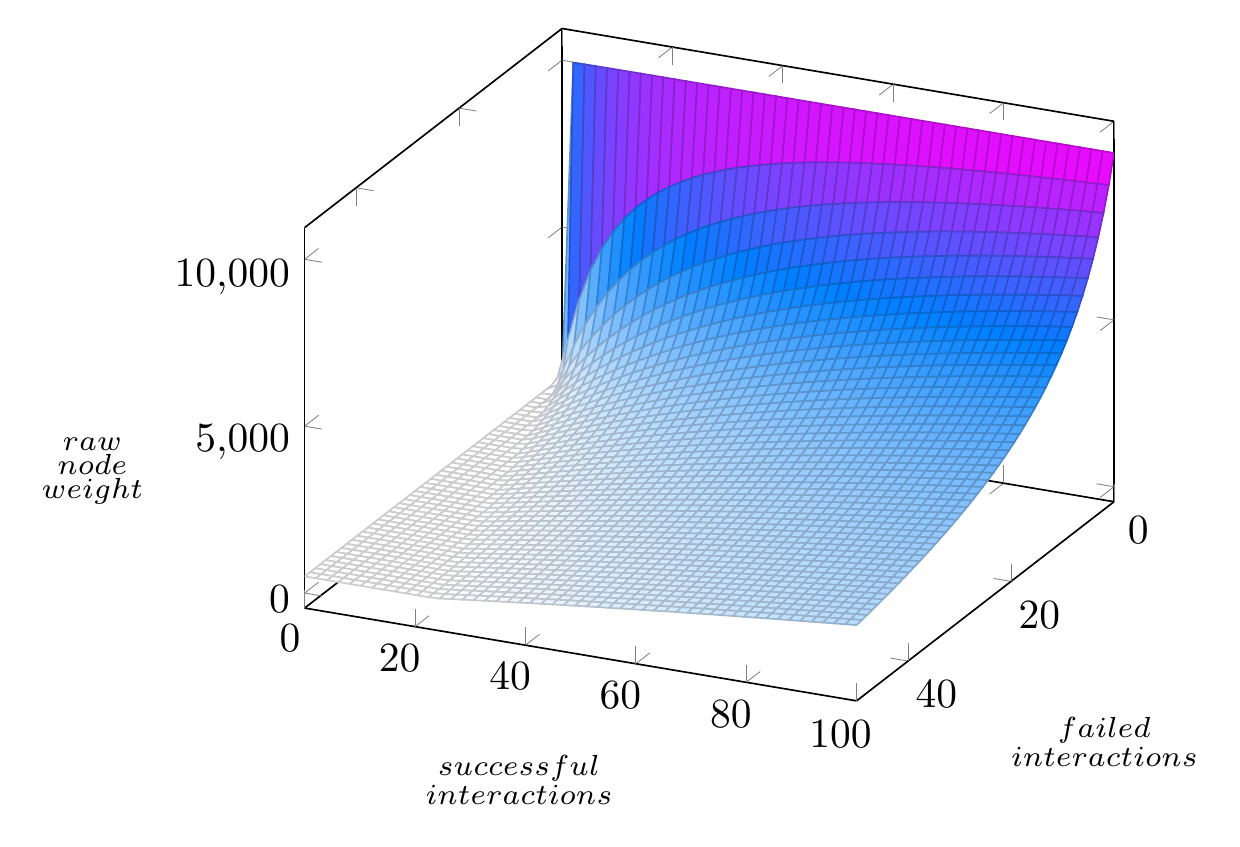
\begin{tikzpicture}[scale=1.5]
					\begin{axis}[
							scaled z ticks=false,
							colormap/cool,
							y dir=reverse,
							zlabel style={rotate=-90},
							xlabel = {$\substack{successful\\interactions}$},
							ylabel = {$\substack{failed\\interactions}$},
							zlabel = {$\substack{raw\\node\\weight}$}
						]
						\addplot3[surf, samples=50, domain=0:100, y domain=50:0] {max(500, x * 10000 / (x + 9 * y))};
					\end{axis}
				\end{tikzpicture}
			}{Raw Node Weight}
		\end{figure}

		\begin{align*}
			\mathvar{rawWeight} = \max\left(500, \frac{s \cdot 10000}{s + 9 \cdot f}\right)
		\end{align*}
	}
\end{itemize}

This formula guarantees that failed interactions rapidly decrease the weight of a remote node and its likelihood of getting selected.
The presence of a minimum score still gives a node with many failures a slight chance for being selected and possibly improving its score with more interactions.

The raw weight is multiplied with a weight multiplier to give the final weight of a node.
For static nodes, the multiplier is 2.
For dynamic nodes, it is 1.
If a node is banned due to consecutive interaction failures \nemrefparens{sec:reputation:NodeBanning}, the multiplier is decreased by 1.
This ensures that a node does not connect to dynamic banned nodes.
The chance of connecting to static banned nodes is reduced by half.

Removal candidates are determined based on their connection age.
Each removal candidate that will be closed is replaced with a connection to a new node so that the node maintains the desired level of connections.
Finally, for each free slot, a candidate node has a chance of getting selected given by:

\begin{align*}
	P(\textrm{node is getting selected}) = \frac{\mathname{node weight}}{\sum\limits_{\substack{candidates\\nodes}} \mathname{candidate node weight}}
\end{align*}

\subsection{Node Banning}
\index{node!banning}
\index{reputation!node banning|see {node, banning}}
\label{sec:reputation:NodeBanning}

In a public network there could be potentially malicious nodes that try to disturb normal processing of the network.
Therefore, if a node considers a remote node malicious, it will prevent connecting to that node and will not accept incoming connections from it.

Banning is applied at node level and is attached to a node's network scoped identifier \nemrefparens{sec:network:discovery}.
A misbehaving node will be immediately banned for a period of \nemsetting{node}{defaultBanDuration}.
Even after a node is no longer actively banned, the local node will remember for some time (\nemsetting{node}{keepAliveDuration}) that the node was behaving badly and treat repeat violations more severely by banning the node for longer periods up to \nemsetting{node}{maxBanDuration}.
During banning, no connections with the banned node will be established.
After banning has expired, the node is treated like a normal interaction partner again.
There are various scenarios where a remote node will get banned.
The penalties vary based on the cause.

\makeatletter
\setlength{\@fptop}{0pt}
\makeatother
\begin{figure}[H]
	\nemcenterwithcaption{
		\begin{tabular}{|c|c|c|c|c|}
			\hline
			& \makecell{Connection\\closed} & \makecell{Remote\\can\\reconnect} & \makecell{Remote\\can be\\selected} & \makecell{Remote\\can send\\data}\\
			\hline
			\makecell{Consecutive\\interaction\\failures} & No & - & \makecell{Yes Static\\No Dynamic} & Yes\\
			\hline
			\makecell{Invalid\\data} & Yes - All\footnotemark & No & No & No\\
			\hline
			\makecell{Exceeded\\read rate} & Yes - All & No & No & No\\
			\hline
			\makecell{Unexpected\\data} & Yes & Yes & \makecell{Yes\\(after reconnect)} & \makecell{Yes\\(after reconnect)}\\
			\hline
		\end{tabular}
	}{Banning Rules}
\end{figure}
\footnotetext{All active connections associated with the misbehaving node are closed immediately, not just the connection triggering the violation.}

\subsubsection*{Consecutive Interaction Failures}
If interactions with the same node fail for too many consecutive times due to networking or stateful failures, it is better to suspend all interactions with that node for some time, hoping the node will behave better in the future.
The number of consecutive interaction failures before the node gets banned as an interaction partner can be configured.
The amount of time the node gets banned is measured in selection rounds and can also be configured.
While the node is banned, it will not be actively selected as an interaction partner, but it still can send new data.
This violation, therefore, only results in a partial ban.

\subsubsection*{Invalid Data}
Data can be invalid in many ways.
For example, if a remote node is on a fork, it might send a new block that does not fit into the local node's chain.
Little forks with a depth of one or two blocks happen frequently.
Though the sent data is invalid, it is not considered malicious because the remote node's internal state was understandably different.
On the other hand, sending data with invalid signatures clearly indicates that the remote node is malicious because signature verification is independent of a node's state.
The same is true for other verification failures that do not depend on the state of a node.
In all those cases, the remote node gets banned.

\subsubsection*{Exceeded Read Data Rate}
Each node monitors the read rates of all sockets accepting data from peers.
This allows a node to detect when a faulty peer is producing an unexpected amount of data.
If the data read during a configured time interval exceeds a maximum, the socket is closed and the node is banned.
The maximum read rate is configurable.

\subsubsection*{Unexpectedly Receiving Data}
There are situations during node communication where the local node is not expecting to receive any data from the remote.
If the remote still sends data in such a situation, it is violating the protocol and the connection is closed.
In this case, the connection is immediately closed but there is no persistent banning of the node.

	\section{Consensus}
\label{sec:consensus}

\pgfplotsset{consensusAxisBasicStyle/.style={
	axis lines = center,
	scaled x ticks = false,
	scaled y ticks = false,
	legend columns = 3,
	xmin = 0,
	height = 5cm,
	width=(4 * \textwidth) / 5,
}}

\pgfplotsset{consensusAxisEvStyle/.style={
	consensusAxisBasicStyle,
	xlabel = P,
	ylabel = EV,
	ymin = -150,
	ymax = 150,
}}

\nemquote{%
You know what, sometimes it seems to me we’re living in a world that we fabricate for ourselves.
We decide what’s good and what isn’t, we draw maps of meanings for ourselves...
And then we spend our whole lives struggling with what we have invented for ourselves.
The problem is that each of us has our own version of it, so people find it hard to understand each other.
}{Olga Tokarczuk}

\nemchapterfirstletter{B}{yzantine} consensus is a key problem faced by all decentralized systems.
Essentially, the crux of the problem is finding a way to get independent actors to cooperate without cheating.
Bitcoin's key innovation was a solution to this problem that is based on Proof of Work (PoW).
After each new block is accepted into Bitcoin's main chain, all miners begin a competition to find the next block.
All miners are incentivized to extend the main chain instead of forks because the chain with the greatest cumulative hashing power is the reference chain.
Miners calculate hashes as quickly as possible until one produces a candidate block with a hash below the current network difficulty target.
A miner's probability of mining a block is proportional to the miner's hash rate relative to the network's total hash rate.
This necessarily leads to a computational arms race and uses a lot of electricity.

Proof of Stake (PoS)\cite{King:2012:PPP}\cite{Nxt2013} blockchains were introduced after Bitcoin.
They presented an alternative solution to the Byzantine consensus problem that did not require significant power consumption.
Fundamentally, these chains behaved similarly to Bitcoin with one important difference.
Instead of predicating the probability of creating a block on a node's relative hash rate the probability is based on a node's relative stake in the network.
Since richer accounts are able to produce more blocks than poorer accounts, this scheme tends to allow the rich to get richer.

\codenamespace uses a modified version of PoS that borrows key concepts from Proof of Importance (PoI).
This new weighting attempts to capture the original intent of PoI, which was to award \emph{users} preferentially relative to \emph{hoarders}, but not suffer from the scaling issues inherent in the original PoI algorithm.

There are multiple factors that contribute to a healthy ecosystem.
All else equal, accounts with larger stakes making more transactions and running nodes have more skin in the game and should be rewarded accordingly.
Firstly, accounts with larger balances have larger stakes in the network and have greater incentives to see the ecosystem as a whole succeed.
The amount of the currency an account owns is a measure of its stake.
Secondly, accounts should be encouraged to use the network by making transactions.
Network usage can be approximated by the total amount of fees paid by an account.
Thirdly, accounts should be encouraged to run nodes to strengthen the network.
This can approximated by the number of times an account is the beneficiary of a block
\footnote{
	This measure is strongly correlated with stake when all accounts are actively running nodes.
	Its intent is to differentiate accounts running nodes from accounts idling.
}.
Since the node owner has complete control over defining its beneficiary, any benevolent node owner can alternatively boost this measure for a third-party.

Importances are recalculated every \nemsetting{network}{importanceGrouping} blocks.
This reduces the pressure on the blockchain because the importance calculation is relatively expensive and processing it every block would be prohibitive.
Additionally, recalculating importances periodically allows for automatic state aging.
Overall, it is beneficial to calculate importances periodically rather than every block.

In order to encourage good behavior, accounts active in an older time period should not obtain an eternal advantage due to their previous virtuous behavior.
Instead, importance boosts granted by transaction and node scores are time limited.
The boost lasts for five \nemsetting{network}{importanceGrouping} intervals.

\subsection{Weighting Algorithm}
\label{sec:consensus:weighting}

All accounts that have a balance of at least \nemsetting{network}{minHarvesterBalance} participate in the importance calculation and are called \emph{high value accounts}.
Notice that this set of accounts is a superset of the set of accounts eligible for block generation \nemrefparens{sec:blockchain:generation}.
In other words, a nonzero importance at the most recent importance recalculation is a necessary but not sufficient condition for block generation.

An account's \emph{importance score} is calculated by combining three component scores: stake, transaction and node.

The stake score, $S_A$, for an account $A$ is the percentage of currency it owns relative to the total currency owned by all high value accounts.
This percentage is no less than the percentage of currency the account owns relative to all outstanding currency.
Let $B_A$ represent the amount of currency owned by account $A$.
The stake score for account $A$ is calculated for each eligible account as follows:

\begin{equation}
S_A = \frac{B_A}{\sum\limits_{\substack{a \in \mathname{high value accounts}}} B_a}
\end{equation}

The transaction score, $T_A$, for an account $A$ is the percentage of transaction fees it has paid relative to all fees paid by high value accounts within a time period $P$.
Let $\mathfunc{FeesPaid}{A}$ represent the amount of fees paid by $A$ in the time period $P$.
The transaction score for account $A$ is calculated for each eligible account as follows:

\begin{equation}
T_A = \frac{\mathfunc{FeesPaid}(A)}{\sum\limits_{\substack{a \in \mathname{high value accounts}}} \mathfunc{FeesPaid}(a)}
\end{equation}

The node score, $N_A$, for an account $A$ is the percentage of times it has been specified as a beneficiary relative to the total number of high value account beneficiaries within a time period $P$.
Let $\mathfunc{BeneficiaryCount}{A}$represent the number of times $A$ has been specified as a beneficiary in the time period $P$.
The node score for account $A$ is calculated for each eligible account as follows:

\begin{equation}
N_A = \frac{\mathfunc{BeneficiaryCount}(A)}{\sum\limits_{\substack{a \in \mathname{high value accounts}}} \mathfunc{BeneficiaryCount}(a)}
\end{equation}

Together, the transaction and node scores are called the \emph{activity score} because they are both dynamic and derived from an account's activity as opposed to its stake.
The transaction score is weighted at 80\% and the node score at 20\%.
Additionally, the combined score is scaled relative to an account's balance so that there is a dampening effect of activity on importance as stake increases
\footnote{The activity score is rescaled after dampening so that it contributes the desired \nemsetting{network}{importanceActivityPercentage} to the importance calculation.}.
This effectively allows active smaller accounts to gain an outsized boost relative to active larger accounts.
This partially redistributes importance away from rich accounts towards poorer accounts and somewhat counteracts the rich getting richer phenomenon inherent in PoS.
The prominence of activity relative to stake can be configured by \nemsetting{network}{importanceActivityPercentage}.
When this value is zero, \codenamespace behaves like a pure PoS blockchain.
Setting this to too a high value could weaken blockchain security by lowering the cost for an attacker to obtain majority importance and execute a 51\% attack.

As a performance optimization, activity information is only collected for accounts that are \emph{high value} at the time of the most recent importance calculation.
Between importance recalculations, new data is stored in a working bucket.
At each importance recalculation, existing buckets are shifted, the working bucket is finalized and a new working bucket is created.
Each bucket influences at most five importance recalculations.
As a result, activity information quickly expires.

\begin{figure}[ht]
	\nemcenterwithcaption{
		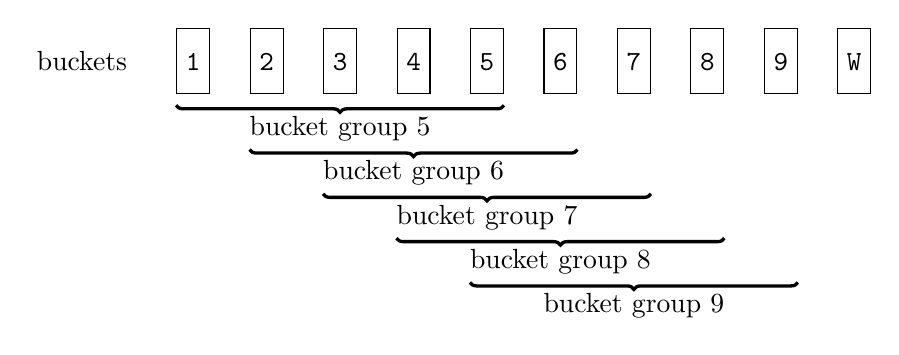
\begin{tikzpicture}[node distance=0.2cm and 0.5cm]
			\node[anchor=center] (lbl1) {buckets};
			\node[crecb,right=of lbl1] (bucket1) {\texttt{1}};
			\node[crecb,right=of bucket1] (bucket2) {\texttt{2}};
			\node[crecb,right=of bucket2] (bucket3) {\texttt{3}};
			\node[crecb,right=of bucket3] (bucket4) {\texttt{4}};
			\node[crecb,right=of bucket4] (bucket5) {\texttt{5}};
			\node[crecb,right=of bucket5] (bucket6) {\texttt{6}};
			\node[crecb,right=of bucket6] (bucket7) {\texttt{7}};
			\node[crecb,right=of bucket7] (bucket8) {\texttt{8}};
			\node[crecb,right=of bucket8] (bucket9) {\texttt{9}};
			\node[crecb,right=of bucket9] (bucketW) {\texttt{W}};

			\draw[decorate,decoration={brace,mirror},very thick]
				([yshift=-4pt] bucket1.south west)
				-- node[below] (xd1) {bucket group 5}
				([yshift=-4pt] bucket5.south east);

			\draw[decorate,decoration={brace,mirror},very thick]
				([yshift=-20pt] bucket2.south west)
				-- node[below] {bucket group 6}
				([yshift=-20pt] bucket6.south east);

			\draw[decorate,decoration={brace,mirror},very thick]
				([yshift=-36pt] bucket3.south west)
				-- node[below] {bucket group 7}
				([yshift=-36pt] bucket7.south east);

			\draw[decorate,decoration={brace,mirror},very thick]
				([yshift=-52pt] bucket4.south west)
				-- node[below] {bucket group 8}
				([yshift=-52pt] bucket8.south east);

			\draw[decorate,decoration={brace,mirror},very thick]
				([yshift=-68pt] bucket5.south west)
				-- node[below] {bucket group 9}
				([yshift=-68pt] bucket9.south east);
		\end{tikzpicture}
	}{Activity buckets}
\end{figure}

The \nemsetting{network}{totalChainImportance} setting specifies the total importance that is distributed among all accounts in a network.
Given that, the spot importance of the account $A$, $I'_A$, can be calculated as follows
\footnote{
	There is some additional edge case handling that is not reflected in the equation around how zero component scores are handled.
	If either the transaction or node scores is zero, the other will be scaled up and serve as the fully weighted activity score.
	If both are zero, the stake score will be scaled up and used exclusively.
}:
\begin{align*}
	\gamma = \: & \nemsetting{network}{importanceActivityPercentage} \\
	\mathvar{ActivityScore}'_A = \: & \frac{\nemsetting{network}{minHarvesterBalance}}{B_A} \cdot \left( 0.8 \cdot T_A + 0.2 \cdot N_A \right) \\
	\mathvar{ActivityScore}_A = \: & \frac{ActivityScore'_A}{\sum\limits_{\substack{a \in \mathname{high value accounts}}} ActivityScore'_a} \\
	I'_A = \: & \nemsetting{network}{totalChainImportance} \cdot \left( \left(1 - \gamma \right) \cdot S_A + \gamma \cdot ActivityScore_A \right)
\end{align*}

The final importance score, $I_A$ for account $A$ is calculated as the minimum of $I'_A$ at the current and previous importance calculations.
This serves as a precaution against a stake grinding attack and a general incentive to minimize unnecessary stake movement.
There is no rescaling, so the sum of $I_A$ for all high value accounts might be less than \nemsetting{network}{totalChainImportance}.

\subsection{Sybil Attack}
\index{sybil attack}

A \emph{Sybil attack} on a peer-to-peer network occurs when an attacker creates multiple identities in order to gain a disproportionately large influence over the network or some other advantage.
In \codename, an attacker might attempt such an attack to boost importance.
Each component of the importance score needs to be robust against such attacks.

As described in \nemref{sec:consensus:weighting}, an account's activity score is dampened relative to its balance.
Accordingly, splitting an account's balance among multiple accounts will lower the average dampening factor applied.
Assuming a constant level of activity is \emph{sustained} before and after redistribution, the cumulative importance will be higher post split
\footnote{
	This assumes that only one account splits.
	The effect is lessened when multiple accounts split because activity scores are relative.
}.
This effect is by design and encourages virtuous behavior because the importance boost is only realized if activity is sustained.
Preservation of the transaction score encourages transacting and paying fees from multiple accounts.
Preservation of the node score encourages running additional nodes and connecting them to the network.

Assume $\mu := \nemsetting{network}{minHarvesterBalance}$ and an attacker that owns $N \cdot \mu$ total currency.
Consider two extremes:

\begin{enumerate}
	\item{The attacker has a single account with $N \cdot \mu$ currency}
	\item{The attacker has $N$ accounts with $\mu$ currency}
\end{enumerate}

\subsubsection*{Boosting Stake Score}

In both extremes, the total currency owned by the attacker is the same.
Accordingly, the stake score is the same and there is no benefit gained from splitting accounts.
For emphasis:

\begin{equation}
B_A = \sum\limits_{a \in \{1, \dotso, N\}} B_a
\end{equation}

\subsubsection*{Boosting Node Score}

\codenamespace allows a node owner to specify a beneficiary for every block harvested on their node.
Each time an account is specified as a beneficiary, assuming it is already a \emph{high value account}, it will get a slight boost in its node score.

In both extremes, the total beneficiary count for the attacker is the same.
Accordingly, the node score is the same and there is no undeserved benefit gained from splitting accounts.
For emphasis:

\begin{equation}
\mathfunc{BeneficiaryCount}(A) = \sum\limits_{a \in \{1, \dotso, N\}} \mathfunc{BeneficiaryCount}(a)
\end{equation}

The attacker might obtain a higher node score if running more nodes allows the attacker's nodes to host more delegated harvesters.
This is not a bad outcome and by design.
It encourages more nodes in the network, which is a good thing that strengthens the network.

The attacker could try to cheat by setting up $N$ virtual nodes pointing to a single physical machine.
Each of these virtual nodes would be treated by the rest of the network as a normal node, and the underlying physical node would be interacted with $N$ times more often than a normal node in the network.
This implies that the virtual nodes are running on a strong physical server, which is still beneficial to the network relative to a weaker physical server.

\subsubsection*{Boosting Transaction Score}

The transaction score is solely based on fees.
There is no difference between one huge account spending $X$ on fees and $N$ smaller accounts each spending $\frac{X}{N}$ on fees.
For emphasis:

\begin{equation}
\mathfunc{FeesPaid}(A) = \sum\limits_{a \in \{1, \dotso, N\}} \mathfunc{FeesPaid}(a)
\end{equation}

The only possibility to boost transaction score is a \emph{fee attack}, which is discussed in detail in \nemref{sec:consensus:feeAttack}.

\subsection{Nothing At Stake Attack}

A general criticism of PoS consensus is the \emph{nothing at stake} attack.
This attack theoretically exists when the opportunity cost of creating a block is negligible.
There are two variations of this attack.

In the first variation, all harvesters except the attacker harvest on all forks.
Simplifying the description to assume a binary fork, the attacker would submit a payment to one branch and immediately start harvesting on the other branch.
Assuming the attacker has sufficient importance to harvest blocks, eventually the branch without the attacker's payment will become the reference chain because it will have a a higher score
\footnote{This assumes that there is only a single attacker or all attackers collude to withhold harvesting from the same branch.}.
The attacker's payment is not included in this branch, so the attacker's funds are effectively returned.

There are three primary defenses against this attack.
First, the attacker has a limited amount of time to produce a better chain because at most \nemsetting{network}{maxRollbackBlocks} blocks can be rolled back.
If the merchant waits to render services until at least this many blocks are confirmed, the attack is impossible.
Second, in order to execute a successful nothing at stake attack, the attacker must own a significant importance in the network
\footnote{
	Theoretically, an attacker would need just \nemsetting{network}{minHarvesterBalance} to execute this attack.
	In practice, in order to guarantee successful execution, the attacker would need a large enough importance to always harvest a block within the rollback interval.
}.
Third, successful execution of this attack against the network will likely have a negative influence on the currency value.
Since other harvesters, by harvesting on all forks, enable this attack, profit-maximizing harvesters should only harvest on a single chain to preclude it.

In the second variation, a single attacker harvests on all forks and attempts to capture all fees irrespective of which chain becomes the reference chain.
An attacker could harvest on all forks starting from the second block searching for the chain in which the attacker has harvested the most fees.
Since block acceptance is probabilistic, in theory, an attacker could spend infinite time building the perfect chain in which the attacker has harvested all blocks.

Most theoretical nothing at stake attacks imagine an idealized blockchain and ignore protocol-level safeguards that protect against such attacks.
In practice, this type of attack is impractical if the attacker owns a minority of currency.
The aforementioned two defenses are also applicable here.
In addition, changes in block difficulty \nemrefparens{sec:blockchain:difficulty} are capped at 5\%.
It will take some time for the difficulty of the attacker's chain to adjust downward, which will cause the block times at the beginning of the secret chain to significantly lag those of the main chain.
These large time differences will make it unlikely for the attacker to produce a chain with a better score \nemrefparens{sec:blockchain:score}.

A small amount of stake aging also decreases the likelihood of this second variation.
Requiring accounts to have nonzero importances for two consecutive importance recalculations as a precondition for harvesting makes generation hash grinding\footnote{This is an attempt to brute force the block hit \nemrefparens{sec:blockchain:generation}, which is dependent on generation hash.} attacks nonviable.
In order to exploit this, the attacker would need to move all currency to a specific account more than \nemsetting{network}{importanceGrouping} blocks before the attack could be carried out.
Since the attacker can't know all the blocks that will be confirmed in the intervening period, such movement cannot result in any benefit.

\subsection{Fee Attack}
\label{sec:consensus:feeAttack}

A \emph{fee attack} is an attempt by an attacker to exploit the transaction score by paying large fees in order to boost its own importance.
The attack is considered effective if it yields a positive expected value.

The analysis in this section will be performed using recommended public network settings.
These include \nemsetting{network}{totalChainImportance} equal to 9 billion, \nemsetting{network}{importanceGrouping} equal to 359 blocks and \nemsetting{minHarvesterBalance} equal to 10000 currency.
Additionally, \nemsetting{network}{importanceActivityPercentage} is 5, so the cumulative transaction score accounts for 4\% of importance.

\subsubsection*{Large Account}

Consider an account that is large enough to harvest one block per importance recalculation interval without any activity boosting.
Assuming only 2 of 9 billion currency is actively harvesting, the account will need at least 5.57 million currency to harvest this frequently.

The account might try to make a profit by adding a transaction with a high fee to one of its own harvested blocks each recalculation interval.
This would boost the account's importance and allow it to harvest more blocks in the future and, consequently, collect more fees.
However, this activity is not risk free.
The account risks paying the high fee if a better block replaces its block.
When the original block is unwound, the high fee transaction will enter the unconfirmed transactions cache and be eligible for inclusion in a new block created by a different harvester.
This scenario is a net loss because the account will have to pay the high fee.

Let $P$ be the probability of a fork resulting in a loss, $F$ be the high fee in a block, and $\bar{F}$ be the average fee in a block.
The expected value, $EV$, can be approximated as follows:
\begin{align*}
	\tag{importance boost}\beta &= 0.04 \cdot \frac{1}{557} \cdot \frac{F}{359 \cdot \bar{F} + F} \\
	\tag{expected value} EV &= \beta \cdot \frac{359}{P} \cdot \bar{F} - F
\end{align*}

The expected value is positive for small values of $P$.
As $P$ or $F$ increases, it quickly becomes negative.
Using the recommended public network settings, $P$ needs to be less than 0.0001 for the expected value to be positive.
This implies a fork resulting in a loss occurs less than once every 10000 blocks.
Given the mechanism of distributed consensus, this is a near impossibility.
Small one or two block forks occur quite frequently.

\begin{figure}[H]
	\nemcenterwithcaption{
		\begin{tikzpicture}[trim axis left]
			\begin{axis}[consensusAxisEvStyle, xtick distance=0.000025, xmax = 0.0001]
				\addplot[color=red,domain=0:0.0001]{(0.04 / 557 * 100 / (359 * 0.1 + 100)) * (359 / x) * 0.1 - 100};
				\addlegendentry{$\bar{F} = 0.1$}

				\addplot[color=green,domain=0:0.0001]{(0.04 / 557 * 100 / (359 * 1 + 100)) * (359 / x) * 1 - 100};
				\addlegendentry{$\bar{F} = 1$}

				\addplot[color=blue,domain=0:0.0001]{(0.04 / 557 * 100 / (359 * 10 + 100)) * (359 / x) * 10 - 100};
				\addlegendentry{$\bar{F} = 10$}
			\end{axis}
		\end{tikzpicture}
	}{Fee attack large account analysis (F = 100)}
\end{figure}

\subsubsection*{Small Account}

Consider an account that has a balance equal to \nemsetting{network}{minHarvesterBalance}.
Assume the account makes one transaction with high fees in two consecutive recalculation intervals.
These fees are lost to other harvesters because the probability of the account harvesting a block is quite small.
The high fees paid boost the account’s importance enough so that it is able to harvest at least one block per importance recalculation interval.
From this point forward, the account behaves like the large account in the previous section.
It will also add a transaction with a high fee to one of its own harvested blocks each recalculation interval.
The account hopes that due to the increased probability of harvesting a block, its additional collected fees will exceed its costs.

\begin{figure}[H]
	\nemcenterwithcaption{
		\begin{tikzpicture}[trim axis left]
			\begin{axis}[consensusAxisEvStyle, xtick distance=0.01, xmax = 0.04]
				\addplot[color=red,domain=0:0.04]{(0.04 / 557 * 100 / (359 * 1 + 100)) * (359 / x) * 1 - 100};
				\addlegendentry{large}

				\addplot[color=green,domain=0:0.04]{(0.04 / 56 * 100 / (359 * 1 + 100)) * (359 / x) * 1 - 100};
				\addlegendentry{medium}

				\addplot[color=blue,domain=0:0.04]{(0.04 * 100 / (359 * 1 + 100)) * (359 / x) * 1 - 100};
				\addlegendentry{small}
			\end{axis}
		\end{tikzpicture}
	}{Fee attack balance sensitivity (F = 100, $\bar{F} = 1$)}
\end{figure}

Let $P$ be the probability of a fork resulting in a loss, $F$ be the high fee in a block, and $\bar{F}$ be the average fee in a block.
The expected value, $EV$, excluding the initial transaction fees, can be approximated as follows\footnote{
The difference relative to the large account example is that the damping factor is completely removed.}:
\begin{align*}
	\tag{importance boost}\beta &= 0.04 \cdot \frac{F}{359 \cdot \bar{F} + F} \\
	\tag{expected value} EV &= \beta \cdot \frac{359}{P} \cdot \bar{F} - F
\end{align*}

The expected value is positive for larger values of $P$ than in the large account scenario.
A fee attack confers an outsized benefit to a small account relative to a large account because the activity scores of the latter are dampened more aggressively than those of the former.
Specifically, a damping factor of $\frac{1}{557}$ is applied to the large account's activity score, but no damping factor is applied to the small account's activity score.

The expected value increases as $\bar{F}$ increases.
As $P$ or $F$ increases, it quickly becomes negative.
Using the recommended public network settings, $P$ needs to be less than 0.05 for the expected value to be positive.
This implies a fork resulting in a loss occurs less than once every 20 blocks.
Given the mechanism of distributed consensus, this is possible.

\begin{figure}[H]
	\nemcenterwithcaption{
		\begin{tikzpicture}[trim axis left]
			\begin{axis}[consensusAxisEvStyle, xtick distance=0.01, xmax = 0.04]
				\addplot[color=red,domain=0:0.04]{(0.04 * 100 / (359 * 0.1 + 100)) * (359 / x) * 0.1 - 100};
				\addlegendentry{$\bar{F} = 0.1$}

				\addplot[color=green,domain=0:0.04]{(0.04 * 100 / (359 * 1 + 100)) * (359 / x) * 1 - 100};
				\addlegendentry{$\bar{F} = 1$}

				\addplot[color=blue,domain=0:0.04]{(0.04 * 100 / (359 * 10 + 100)) * (359 / x) * 10 - 100};
				\addlegendentry{$\bar{F} = 10$}
			\end{axis}
		\end{tikzpicture}
	}{Fee attack small account analysis (F = 100)}
\end{figure}

\subsubsection*{Further Discussion}

Although a single small account can obtain a positive expected value by executing this attack, the payoff decreases as multiple accounts attempt it simultaneously.
Since there is a positive expected value, profit maximizing actors should all attempt this attack.
As more accounts attempt it, the importance boost obtained by each individual account decreases rapidly and, consequently, the expected value also decreases.\footnote{
	As more accounts produce high fee transactions to attempt this attack, $\bar{F}$ increases.
	For large numbers of attackers, if $F$ is not raised in proportion, the expected value of the attack can increase even though the importance boost per account decreases.
	This is an expected outcome since the value of blocks also increases significantly.
}.

Additionally, there is an upper limit on the number of small accounts that can execute this attack simultaneously.
In order for this attack to be successful, an account needs to be able to to harvest at least one block per importance recalculation interval.
This presupposes the small account can boost its importance score by exploiting the transaction score component.
There is a theoretical limit on the number of accounts that can achieve a significant enough boost because both the importance allotted to the transaction score and the recalculation interval are finite.
Considering the recommended public network settings, this limit is approximately $0.04 \div \frac{1}{359} \approx 14.36$ accounts.

Let $N$ be the number of small accounts attempting the attack, $P$ be the probability of a fork resulting in a loss, $F$ be the high fee in a block, and $\bar{F}$ be the average fee in a block.
The expected value, $EV$, can be approximated as follows:
\begin{align*}
	\tag{importance boost}\beta &= 0.04 \cdot \frac{F}{359 \cdot \bar{F} + N \cdot F} \\
	\tag{expected value} EV &= \beta \cdot \frac{359}{P} \cdot \left( \bar{F} + \frac{\left( N - 1\right ) \cdot F \cdot P}{359} \right) - F
\end{align*}

\begin{figure}[H]
	\nemcenterwithcaption{
		\begin{tikzpicture}[trim axis left]
			\begin{axis}[consensusAxisEvStyle, xtick distance=0.01, xmax = 0.04]
				\addplot[color=red,domain=0:0.04]{(0.04 * 100 / (359 * 1 + 100)) * (359 / x) * (1 + 0) - 100};
				\addlegendentry{one}

				\addplot[color=green,domain=0:0.04]{(0.04 * 100 / (359 * 1 + 2 * 100)) * (359 / x) * (1 + 1 * 100 * x / 359) - 100};
				\addlegendentry{two}

				\addplot[color=blue,domain=0:0.04]{(0.04 * 100 / (359 * 1 + 8 * 100)) * (359 / x) * (1 + 7 * 100 * x / 359) - 100};
				\addlegendentry{eight}
			\end{axis}
		\end{tikzpicture}
	}{Fee attack declining with more attackers (F = 100, $\bar{F} = 1$)}
\end{figure}

	\section{Finalization}
\label{sec:finalization}

\nemquote{%
And it feels like, finally.
}{Patrick Ness}

The CAP Theorem posits that, in the presence of a network failure or partition,
a distributed system must choose either \emph{consistency} or \emph{availability}.

In a consistent system, requests sent to two nodes will always return the same value.
If the value is not globally agreed upon, the request will fail.
This ensures that all clients have a uniform view of the system.
BFT systems typically choose consistency and risk network stalls.
A naive consistent system could require all stakeholders to vote on each block
and only allow the next block when $\frac{2}{3}$ of stakeholders approve.
If stakeholders fail to vote promptly, there could be a delay in block production.

In an available system, requests sent to two nodes will always return a value immediately.
The returned values can be different, so different clients could have different views of the system.
PoW and NXT-style PoS systems typically chose availability and eventual consensus.
They risk propagating different (potentially unresolvable) views of the system.
Available PoW-like systems, like Bitcoin, have a simple fork rule that chooses the chain with the most work.
If the network is split into partitions with equal hash power, all partitions will proceed independently without knowing they’re partitioned.
When they are eventually reconnected, there will be an expensive (and potentially deep) fork resolution.

\codenamespace always prefers availability over consistency, but it optionally supports the use of a finality gadget on top of its native consensus \nemrefparens{sec:consensus}.
This gadget introduces a BFT-inspired voting system that is orthogonal to block production and block consensus.
As a result of its optionality, \codenamespace is able to support networks that use either deterministic finalization (when the gadget is enabled) or probabilistic finalization (when the gadget is disabled).
The gadget is automatically enabled when \nemsetting{node}{maxRollbackBlocks} is zero\footnote{
	The finalization extension must also be enabled.
}.

The gadget approach is modeled after GRANDPA \cite{Stewart2020grandpa} used by Polkadot.
GRANDPA, in turn, in influenced by CASPER \cite{CasperFfg}, which itself is influenced by PBFT \cite{Pbft1999}.
Traditionally, PBFT uses three types of messages: pre-prepare, prepare and commit.
Pre-prepare messages, which are used to start rounds, are not used in \codenamespace.
Instead, elapsed network time \nemrefparens{sec:timesync} is used to start rounds.
Prepare and commit messages in PBFT roughly correspond to prevote and precommit messages in \codenamespace.

\subsection{High Level Overview}

Block finalization is a complicated process that involves two types of messages: prevotes and precommits.
At the beginning of a round, each voter only knows the blocks stored in its local chain.
No voter knows the blocks stored in the chains of any other voter.
Consequently, it is impossible for a voter to know which of its blocks will receive a supermajority of votes and be finalized ahead of time.

To illustrate the general procedure of finalization, consider a network composed of three equally weighted voters.
A supermajority requires at least two of the three voters to vote for the same hash.
$F$ refers to the last finalized block.

\begin{figure}[H]
	\nemcenter{
		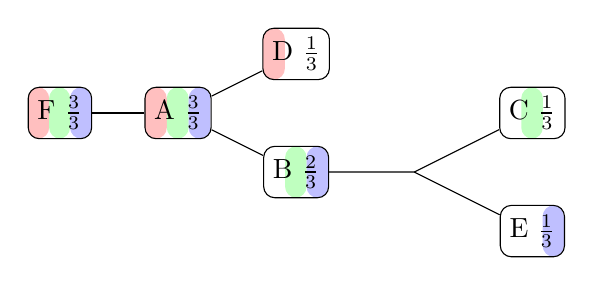
\begin{tikzpicture}[every node/.style = {shape=rectangle, rounded corners, draw, align=center}]
			\tikzset{
				fill fraction/.style n args={3}{
					path picture={
						\fill[#1]
							($(path picture bounding box.south west)!#2!(path picture bounding box.south east)$)
							rectangle
							($(path picture bounding box.north west)!#3!(path picture bounding box.north east)$);
					}
				}
			}

			\tikzset{ vote1/.style = { fill fraction={red!25}{0.00}{0.33} } }
			\tikzset{ vote2/.style = { fill fraction={green!25}{0.33}{0.66} } }
			\tikzset{ vote3/.style = { fill fraction={blue!25}{0.66}{0.99} } }

			\tikzset{ vote23/.style = {
					path picture={
						\fill[green!25]
							($(path picture bounding box.south west)!0.33!(path picture bounding box.south east)$)
							rectangle
							($(path picture bounding box.north west)!0.66!(path picture bounding box.north east)$);
						\fill[blue!25]
							($(path picture bounding box.south west)!0.66!(path picture bounding box.south east)$)
							rectangle
							($(path picture bounding box.north west)!0.99!(path picture bounding box.north east)$);
					}
				}
			}

			\tikzset{ vote123/.style = {
					path picture={
						\fill[red!25]
							($(path picture bounding box.south west)!0.00!(path picture bounding box.south east)$)
							rectangle
							($(path picture bounding box.north west)!0.33!(path picture bounding box.north east)$);
						\fill[green!25]
							($(path picture bounding box.south west)!0.33!(path picture bounding box.south east)$)
							rectangle
							($(path picture bounding box.north west)!0.66!(path picture bounding box.north east)$);
						\fill[blue!25]
							($(path picture bounding box.south west)!0.66!(path picture bounding box.south east)$)
							rectangle
							($(path picture bounding box.north west)!0.99!(path picture bounding box.north east)$);
					}
				}
			}

			\node [vote123] {F $\frac{3}{3}$}
			child[grow=right] {
				node [vote123] {A $\frac{3}{3}$}
				child {
					node [vote23] {B $\frac{2}{3}$}
					child {
						child { node [vote3] {E $\frac{1}{3}$} }
						child { node [vote2] {C $\frac{1}{3}$} }
					}
				}
				child { node [vote1] {D $\frac{1}{3}$} }
			};
		\end{tikzpicture}
	}{}
\end{figure}

Subsequently, the voters will be referenced by their colors in the figure \texttt{red}, \texttt{green} and \texttt{blue}.

Finalization is greedy, and it attempts to finalize as many blocks as possible each round.
In the first \emph{prevote stage}, each voter constructs and publishes a hash chain representing its local chain starting with the hash of the last finalized block ($F$).
In this example, the prevote chains will be:

\begin{enumerate}
	\item{\texttt{\space\space red}: $\hf(F)$, $\hf(A)$, $\hf(D)$}
	\item{\texttt{green}: $\hf(F)$, $\hf(A)$, $\hf(B)$, $\hf(C)$}
	\item{\texttt{ blue}: $\hf(F)$, $\hf(A)$, $\hf(B)$, $\hf(E)$}
\end{enumerate}

Assume that \texttt{red}, due to bad network connections, only receives the prevote from \texttt{green} but not \texttt{blue}.
Assume that \texttt{green} and \texttt{blue} receive prevotes from all voters.
At this point, each voter has the following prevote chains:

\begin{enumerate}
	\item{\texttt{\space\space red}:
		\begin{enumerate}
			\item{$\hf(F)$, $\hf(A)$, $\hf(D)$}
			\item{$\hf(F)$, $\hf(A)$, $\hf(B)$, $\hf(C)$}
		\end{enumerate}
	}
	\item{\texttt{green}:
		\begin{enumerate}
			\item{$\hf(F)$, $\hf(A)$, $\hf(D)$}
			\item{$\hf(F)$, $\hf(A)$, $\hf(B)$, $\hf(C)$}
			\item{$\hf(F)$, $\hf(A)$, $\hf(B)$, $\hf(E)$}
		\end{enumerate}
	}
	\item{\texttt{ blue}:
		\begin{enumerate}
			\item{$\hf(F)$, $\hf(A)$, $\hf(D)$}
			\item{$\hf(F)$, $\hf(A)$, $\hf(B)$, $\hf(C)$}
			\item{$\hf(F)$, $\hf(A)$, $\hf(B)$, $\hf(E)$}
		\end{enumerate}
	}
\end{enumerate}

Each voter inspects all prevote hash chains to calculate the best block that \textbf{might} be finalized this round.
\texttt{red} only sees a supermajority for $A$ but \texttt{green} and \texttt{blue} see a supermajority for $B$.
In the next \emph{precommit stage}, each voter publishes the hash of its calculated best block:

\begin{enumerate}
	\item{\texttt{\space\space red}: $\hf(A)$}
	\item{\texttt{green}: $\hf(B)$}
	\item{\texttt{ blue}: $\hf(B)$}
\end{enumerate}

Assume that \texttt{green}, due to bad network connections, only receives the precommit from \texttt{red} but not \texttt{blue}.
Assume that \texttt{red} and \texttt{blue} receive precommits from all voters.
At this point, each voter has the following precommits:

\begin{enumerate}
	\item{\texttt{\space\space red}: $\hf(A)$, $\hf(B)$, $\hf(B)$}
	\item{\texttt{green}: $\hf(A)$, $\hf(B)$}
	\item{\texttt{ blue}: $\hf(A)$, $\hf(B)$, $\hf(B)$}
\end{enumerate}

Each voter inspects all precommit hashes to calculate the best block that can be finalized.
Importantly, a precommit for a block is also a precommit for all of the block's ancestors.
\texttt{green} only sees a supermajority for $A$ but \texttt{red} and \texttt{blue} see a supermajority for $B$.
In the final \emph{commit stage}, each voter finalizes the following blocks:

\begin{enumerate}
	\item{\texttt{\space\space red}: $\hf(A)$, $\hf(B)$}
	\item{\texttt{green}: $\hf(A)$}
	\item{\texttt{ blue}: $\hf(A)$, $\hf(B)$}
\end{enumerate}

The following sections discuss the finalization algorithm in more detail.

\subsection{Rounds}

A \nind{finalization round} represents a step in the finalization process and is composed of a \nind{finalization epoch} and a \nind{finalization point}.

An epoch is a group of blocks.
All blocks within an epoch are finalized by a single voting set, which is recalculated every \nemsetting{network}{votingSetGrouping} blocks.
The first epoch is defined as exclusively containing the nemesis block and is inherently considered to be finalized.
Subsequent epochs must end at a block with a height that is a multiple of \nemsetting{network}{votingSetGrouping}.
An epoch is considered \emph{finalized} when all blocks within it are finalized.
There will always be a finalization proof available for the last block within an epoch.

A point is a fine-grained step within an epoch that represents progress towards finalization of that epoch.
Each point can finalize zero or more blocks.
A point can only finalize blocks within its parent epoch.
This prevents any block from being potentially finalized by multiple voting sets, which could lead to a safety violation.
There is no limit on the number of points associated with an epoch.
There will be as many points as necessary to finalize all blocks within an epoch.
The last point within an epoch will always finalize that epoch's last block.
A block is considered \emph{finalized} when a point finalizes that block or any of its descendants.

When a network is partitioned, it is possible for a point to finalize zero additional blocks.
This happens when only the last finalized block receives a supermajority of votes.
This is not a fatal error and can occur naturally in the presence of network partitions.
Afterwards, the finalization procedure will continue and advance to the next point based on the conditions described in \nemref{sec:finalization:algorithm}.

The important difference between an epoch and a point is their relation to voting sets.
Different epochs may have different voting sets.
Different points within the same epoch must all use the same voting set associated with the epoch.

\begin{figure}[H]
	\nemcenterwithcaption{
		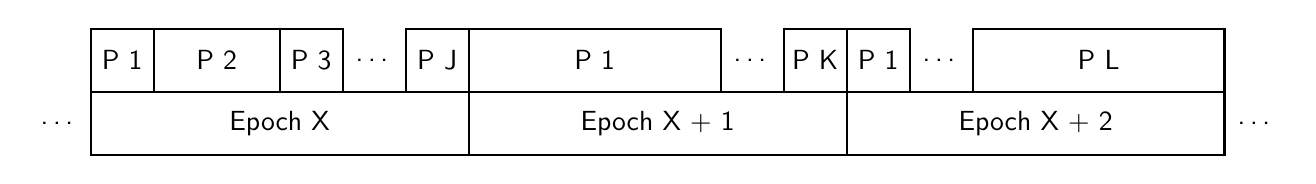
\begin{tikzpicture}[>=latex,font=\sffamily,thick,,scale=0.8, every fit/.style={inner sep=0pt, outer sep=0pt}]
			\tikzstyle{level 3}=[sibling distance=8em]

			\begin{scope}[y=1cm]
				\node [draw=none, fit={(0,0) (1,1)}, label=center:{\ldots}] {};
				\node [draw, fit={(1,0) (7,1)}, label=center:{Epoch X}] {};
				\node [draw, fit={(7,0) (13,1)}, label=center:{Epoch X + 1}] {};
				\node [draw, fit={(13,0) (19,1)}, label=center:{Epoch X + 2}] {};
				\node [draw=none, fit={(19,0) (20,1)}, label=center:{\ldots}] {};
			\end{scope}

			\begin{scope}[yshift=1cm,y=1cm]
				\node [draw, fit={(1,0) (2,1)}, label=center:{P 1}] {};
				\node [draw, fit={(2,0) (4,1)}, label=center:{P 2}] {};
				\node [draw, fit={(4,0) (5,1)}, label=center:{P 3}] {};
				\node [draw=none, fit={(5,0) (6,1)}, label=center:{\ldots}] {};
				\node [draw, fit={(6,0) (7,1)}, label=center:{P J}] {};

				\node [draw, fit={(7,0) (11,1)}, label=center:{P 1}] {};
				\node [draw=none, fit={(11,0) (12,1)}, label=center:{\ldots}] {};
				\node [draw, fit={(12,0) (13,1)}, label=center:{P K}] {};

				\node [draw, fit={(13,0) (14,1)}, label=center:{P 1}] {};
				\node [draw=none, fit={(14,0) (15,1)}, label=center:{\ldots}] {};
				\node [draw, fit={(15,0) (19,1)}, label=center:{P L}] {};
			\end{scope}
		\end{tikzpicture}
	}{Epoch and (P)oint relationship}
\end{figure}

\subsection{Voters}

An account is eligible to vote in a epoch if all of the following are true:
\begin{enumerate}
	\item{Harvesting balance at the last finalized block of the previous epoch is no less than the network defined \nemsetting{network}{minVoterBalance}.}
	\item{Voting key is registered such that \field{StartEpoch} $\leq$ epoch $\leq$ \field{EndEpoch}.}
\end{enumerate}

A voting set for an epoch is the set of all accounts that satisfy the previous conditions.
Importantly, only balance, not importance, is used when weighting votes.
This prevents a safety violation that could occur when using importances\footnote{
	When there are multiple network partitions, each partition would independently recalculate importances with potentially different activity scores.
	Since importances are scaled and not absolute, it's theoretically possible for multiple partitions to have supermajorities of importance and finalize conflicting blocks.
}.

All accounts eligible to vote are expected to vote.
A well-behaved voter is expected to vote in all rounds where it is eligible and not send multiple votes per round.
It is implicitly assumed that all voters will run high-availability nodes and turn on \nemsetting{finalization}{EnableVoting}.
Voters that violate these expectations are considered Byzantine and might be punished in the future.
Votes are weighted proportionally to balance such that the votes from voters with higher balances have more impact.

\subsection{Messages}

Prevote and precommit messages share a common layout.

\begin{figure}[H]
	\nemcenter{
		\nemmemorylayout{
			\begin{leftwordgroup}{\texttt{0x0000}}
				\bitbox{4}{Size} \bitbox{4}{Reserved}
			\end{leftwordgroup} \\
			\nemmemorymultiwordboxskipped{0x0008}{(BM) Signature}{} \\
			\begin{leftwordgroup}{\texttt{0x01B8}}
				\bitbox{4}{Version} \bitbox{4}{\tiny HashesCount}
			\end{leftwordgroup} \\
			\nemmemorysinglewordbox{0x1C0}{StepIdentifier} \\
			\nemmemorysinglewordbox{0x1C8}{Height} \\
			\nemmemorymultiwordboxskipped{0x1D0}{Hashes}{} \\
		}{Message layout}
	}{}
\end{figure}

\index{signature!BM tree}

\field{Signature} is the \emph{BM tree signature} \nemrefparens{sec:cryptography:voting} of the message.
The root public key must match the voting key registered for the message's epoch.
The bottom public key must match the public key in the tree corresponding to the epoch.

\field{Version} is the message version.

\field{Hashes} contains \field{HashesCount} hashes.
A prevote message will contain at least one hash and up to \nemsetting{finalization}{maxHashesPerPoint}.
A precommit message will always contain exactly one hash.

\field{StepIdentifier} indicates the finalization round of the message.
The high bit of the point is reserved to indicate the type of message where 0 indicates prevote and 1 indicates precommit.

\field{Height} is the block height of the first hash contained in \field{Hashes}.

\subsection{Algorithm}
\label{sec:finalization:algorithm}

Define function $g(\ldots)$ to select the last block that has cumulative weighted votes of at least a supermajority of available voting weight.
Define $V_{r,v}$ as a prevote at round $r$ by voter $v$.
Define $C_{r,v}$ as a precommit at round $r$ by voter $v$.
Define $E_{r,v}$ as the estimate by voter $v$ of what might have been finalized in the round $r$.
Notice that this is only an estimate and a greedy one at that.
$E_{r,v}$ must be the latest block on the chain containing $g(V_{r,v})$ that can receive a supermajority of $C_{r,v}$.
A round is \emph{completable} when either:
\begin{enumerate}
	\item{$E_{r,v} < g(V_{r,v})$}
	\item{It is impossible for any child of $g(V_{r,v})$ to have a supermajority of $C_{r,v}$}
\end{enumerate}

A voter $v$ can begin a round $r$ when the previous round is completable, and it has cast votes in all previous rounds where it was eligible.

\subsubsection{Prevote}

When either $1 * \nemsetting{finalization}{stepDuration}$ has elapsed or $r$ is completable, $v$ sends a prevote.

A voter determines the best block that can potentially be finalized.
It creates a prevote message composed of all hashes starting with the hash of the last (local) finalized block.
The prevote message hash chain will contain at most \nemsetting{finalization}{maxHashesPerPoint} hashes.
The last hash in the chain will correspond to a block with a height that is a multiple of \nemsetting{finalization}{prevoteBlocksMultiple}\footnote{
	In practice, \nemsetting{finalization}{maxHashesPerPoint} is expected to be much larger than \nemsetting{finalization}{prevoteBlocksMultiple}.
	Additionally, \nemsetting{network}{votingSetGrouping} should be a multiple of \nemsetting{finalization}{prevoteBlocksMultiple}.
}.
This increases the probability that nodes will send prevote messages with identical chains that can be aggregated more aggressively.

Hashes corresponding to unfinalized blocks are prohibited from spanning epochs.
This guarantees that there is exactly one voting set that can finalize a block at any height.
This property enables dynamic voting sets.

Prevote messages include hash chains, instead of single hashes, because each \codenamespace node stores a single block chain instead of a block tree.
The aggregation of hash chains allows \codenamespace to reconstruct a virtual block tree and apply votes to both seen and unseen branches.

Conceptually, a voter has one vote per height.
Effectively, it votes with its weight on every hash in the prevote hash chain.

\subsubsection{Precommit}

Next, a voter waits until $g(V_{r,v}) \geq E_{r-1,v}$.
When either $2 * \nemsetting{finalization}{stepDuration}$ (relative to the start of the round) has elapsed or $r$ is completable, $v$ sends a precommit.

A voter determines the best block that can potentially be finalized.
It creates a precommit message with a single hash corresponding to $g(V_{r,v})$.

Conceptually, a voter has one vote per height.
Effectively, it votes with its weight on every hash between the last finalized block and the precommit hash.

\subsubsection{Commit}

Asynchronously, a voter collects prevote and precommit messages for round $r$.
In practice, these messages will be associated with either the current round or the previous round.
When $g(C_{r,v})$ changes, that block as well as all blocks between that block and the local finalized block are finalized.

Given a finalization round with epoch $e$ and point $p$, in most cases, the next round will be $(e, p + 1)$.
The one exception to this is when the last block of epoch $e$ is finalized.
In that case, the next round is $(e + 1, 0)$.
Notice that it is possible for both $(e, p + 1)$ and $(e + 1, 0)$ to be started.
In that scenario, $(e + 1, 0)$ will eventually dominate and $(e, p + 1)$ will not complete.

\subsection{Proofs}

In order to minimize network traffic, non-voters do not send or receive individual prevote or precommit messages.
Instead, these nodes pull and individually verify finalization proofs from the network at the end of every epoch.
Upon verification, these nodes finalize the entire epoch at once.

\begin{figure}[H]
	\nemcenterwithcaption{
		\begin{subfigure}{.5\textwidth}
			\nemmemorylayout{
				\begin{leftwordgroup}{\texttt{0x00}}
					\bitbox{4}{Size} \bitbox{4}{Version}
				\end{leftwordgroup} \\
				\nemmemorysinglewordbox{0x08}{Round} \\
				\nemmemorysinglewordbox{0x10}{Height} \\
				\nemmemorymultiwordbox{0x18}{Hash}{3} \\
				\nemmemorymultiwordboxskipped{0x38}{MessageGroups}{} \\
			}{Proof header}
		\end{subfigure}%
		\begin{subfigure}{.5\textwidth}
			\nemmemorylayout{
				\begin{leftwordgroup}{\texttt{0x00}}
					\bitbox{4}{Size} \bitbox{4}{\tiny HashesCount}
				\end{leftwordgroup} \\
				\begin{leftwordgroup}{\texttt{0x08}}
					\bitbox{4}{\tiny Signatures-\\Count} \bitbox{4}{Stage}
				\end{leftwordgroup} \\
				\nemmemorysinglewordbox{0x10}{Height} \\
				\nemmemorymultiwordboxskipped{0x18}{Hashes}{} \\
				\nemmemorymultiwordboxskipped{}{Signatures}{} \\
			}{Message group}
		\end{subfigure}
	}{Finalization proof layouts}
\end{figure}

A finalization proof is composed of a header and a collection of message groups.
The header indicates last block finalized by the proof\footnote{
	Technically, a proof finalizes the last block and all of its ancestors, which are guaranteed to form a single chain.
}.
This block is uniquely identified by its height and hash.
The header also indicates the finalization round at which the block was finalized.

A message group is an aggregation of finalization messages that cryptographically verify the proof.
All finalization messages that differ only in \field{Signature} are grouped together into a single message group with all signatures appended.
There will always be at least two message groups in a proof - one for prevote and one for precommit - but there can be more due to the way votes are counted.

Verification of a finalization proof requires knowledge of the voting set associated with its epoch.
Importantly, the eligible voters and their weights need to be known.
In order to be verified, a proof must only contain valid supporting messages from eligible voters.
Additionally, the messages must indicate that the block specified in the proof header is $g(C_{r,v})$ and $g(V_{r,v}) \geq g(C_{r,v})$.

\subsection{Sybil Attack}

When deterministic finalization is enabled, a \emph{Sybil attack} among voters is prevented by weighting all votes by account balance.
The only way for an attacker to obtain more voting power is to obtain more stake.
Splitting an account's balance across multiple accounts will not change the overall voting power.

\subsection{Nothing at Stake Attack}

When deterministic finalization is enabled, the \emph{nothing at stake attack} can be prevented if a merchant waits to render services until a block is finalized.
If a merchant does not wait, there are additional defenses against this attack.

Most significantly, the attacker has a limited amount of time to produce a better chain.
The attacker must generate a better chain before the network finalizes the block that the attacker wants to rollback.
Additionally, the time required for a significant drop in difficulty will likely be longer than the time it takes to finalize a given chain part.

\subsection{Examples}

\tikzset{ superprevote/.style = {text=white, fill=violet} }
\tikzset{ superprecommit/.style = {text=white, fill=cyan} }

\tikzset{ gprevote/.style = {superprevote, label=below:{$g(V_{r,v})$}} }
\tikzset{ gestimate/.style = {label=below:{\\\\$E_{r,v}$}} }

In all the examples, consider a network with four equally weighted voters.
A supermajority requires at least three of the four voters to vote for the same hash.
$F$ always refers to the last finalized block.
A prevote message cast for a block $B$ implies a prevote hash chain composed of hashes from $F$ to $B$, inclusive.

\subsubsection*{Example 1}

Prevote messages are cast for $A$, $C$, $D$, $E$.
Since $C$ is on the branch of $D$ and $E$, it has a supermajority of votes even though only one voter voted for it explicitly.

\begin{figure}[H]
	\nemcenter{
		\begin{tikzpicture}[every node/.style = {shape=rectangle, rounded corners, draw, align=center}]
			\node [superprevote] {F $\frac{4}{4}$}
			child[grow=right] {
				child {
					node [superprevote] {B $\frac{3}{4}$}
					child {
						node [gprevote] {C $\frac{3}{4}$}
						child {
							child { node {E $\frac{1}{4}$} }
							child { node {D $\frac{1}{4}$} }
						}
					}
				}
				child { node {A $\frac{1}{4}$} }
			};
		\end{tikzpicture}
	}{}
\end{figure}

\subsubsection*{Example 2}

Consider a network split into two equally sized partitions.
Prevote messages are cast for $A$, $A$, $B$, $B$.
Since $F$ is on the branch of $A$ and $B$, it has a supermajority of votes even though no voter voted for it explicitly.
Importantly, notice that no new blocks are finalized because $F$ is already finalized.

\begin{figure}[H]
	\nemcenter{
		\begin{tikzpicture}[every node/.style = {shape=rectangle, rounded corners, draw, align=center}]
			\node [gprevote] {F $\frac{4}{4}$}
			child[grow=right] {
				child { node {B $\frac{2}{4}$} }
				child { node {A $\frac{2}{4}$} }
			};
		\end{tikzpicture}
	}{}
\end{figure}

\subsubsection*{Example 3a}

Prevote messages are cast for $A$, $B$, $C$, $D$ so that $B$ has a supermajority of prevotes.
Assume two voters see prevotes $A$, $B$, $C$ and send precommits for $A$.
Assume one voter sees prevotes $B$, $C$, $D$ and sends a precommit for $B$.
A voter can determine that the weight of unknown precommits (25\%) cannot cause a supermajority of precommits for $B$, which only has 25\% of precommits.
This satisfies condition 1 in \nemref{sec:finalization:algorithm}.

\begin{figure}[H]
	\nemcenter{
		\begin{tikzpicture}[every node/.style = {shape=rectangle, rounded corners, draw, align=center}]
			\node [superprecommit] {F $\frac{4}{4}\frac{3}{4}$}
			child[grow=right] {
				node [superprecommit, gestimate] {A $\frac{4}{4}\frac{3}{4}$}
				child {
					node [gprevote] {B $\frac{3}{4}\frac{1}{4}$}
					child {
						node {C $\frac{2}{4}$}
						child {
							node {D $\frac{1}{4}$}
						}
					}
				}
			};
		\end{tikzpicture}
	}{}
\end{figure}

\subsubsection*{Example 3b}

Consider a slight modification of the previous example where prevotes are received in a different order.
As above, prevote messages are cast for $A$, $B$, $C$, $D$ so that $B$ has a supermajority of prevotes.
Assume two voters see prevotes $B$, $C$, $D$ and send precommits for $B$.
Assume one voter sees prevotes $A$, $B$, $C$ and sends a precommit for $A$.
A voter can determine that the weight of unknown precommits (25\%) cannot cause a supermajority of precommits for $C$, which only has 0\% of precommits.
This satisfies condition 2 in \nemref{sec:finalization:algorithm}.

\begin{figure}[H]
	\nemcenter{
		\begin{tikzpicture}[every node/.style = {shape=rectangle, rounded corners, draw, align=center}]
			\node [superprecommit] {F $\frac{4}{4}\frac{3}{4}$}
			child[grow=right] {
				node [superprecommit] {A $\frac{4}{4}\frac{3}{4}$}
				child {
					node [gprevote, gestimate] {B $\frac{3}{4}\frac{2}{4}$}
					child {
						node {C $\frac{2}{4}$}
						child {
							node {D $\frac{1}{4}$}
						}
					}
				}
			};
		\end{tikzpicture}
	}{}
\end{figure}

\subsubsection*{Example 4}

Consider an extension of the previous example where $A$ is committed at point $r-1$ but $B$ is not.
Now, the voters have moved to the next point $r$.
Four prevote messages and four precommit messages are cast for $F$.
Blocks $B$, $C$, $D$ have all been pruned from the main chain even though precommits for $B$ were used to commit $A$ at $r-1$.
In order to verify the proof at $r-1$, there needs to be a record that $B$ is a descendant of $A$.
This information is stored in the prevote message hash chains but not in the precommit messages.
This is why the verification of finalization proofs requires prevotes.

\begin{figure}[H]
	\nemcenter{
		\begin{tikzpicture}[every node/.style = {shape=rectangle, rounded corners, draw, align=center}]
			\tikzset{ pruned/.style = {color=gray} }

			\node [superprecommit] {F $\frac{4}{4}\frac{4}{4}$}
			child[grow=right] {
				node [superprecommit, label=below:{$g(C_{r-1,v})$}] {A $\frac{4}{4}\frac{4}{4}$}
				child {
					node [superprecommit] {E $\frac{4}{4}\frac{4}{4}$}
					child {
						node [gprevote, gestimate] {F $\frac{4}{4}\frac{4}{4}$}
					}
				}
				child {
					node [pruned] {B}
					child {
						node [pruned] {C}
						child {
							node [pruned] {D}
						}
					}
				}
			};
		\end{tikzpicture}
	}{}
\end{figure}

	\section{Time Synchronization}
\label{sec:timesync}

\nemquote{%
Time and Tide wait for no man.
}{Geoffrey Chaucer}

\nemchapterfirstletter{L}{ike} most other blockchains, \codenamespace relies on timestamps for transactions and blocks.
Ideally, all nodes in the network should be synchronized with respect to time.
Even though most modern operating systems have time synchronization integrated,
nodes can still have local clocks that deviate from real time by more than a minute.
This causes those nodes to reject valid transactions or blocks, which makes it impossible for them to synchronize with the network.

It is therefore needed to have a synchronization mechanism to ensure all nodes agree on time.
There are basically two ways to do this:
\begin{enumerate}
\item Use an existing protocol, such as NTP
\item Use a custom protocol
\end{enumerate}

The advantage of using an existing protocol like NTP is that it is easy to implement and the network time will always be near real time.
This has the disadvantage that the network relies on servers outside the network.

Using a custom protocol that only relies on the P2P network itself solves this problem, but there is a trade off.
It is impossible to guarantee that the network time is always near real time.
For an overview of different custom protocols see \cite{Scipioni2009}.
\codenamespace uses a custom protocol based on Chapter 3 of this thesis in order to be completely independent from any outside entity.
The protocol is implemented in the timesync extension.

\subsection{Gathering Samples}
\index{time offset}

Each node in the network manages an integer \emph{offset} that is set to 0 at start.
The local system time in milliseconds adjusted by the offset (which can be negative) is the \nind{network time} (again in milliseconds) of the node.

After the start up of a node is completed, the node (hereafter called \emph{local node}) selects partner nodes for performing a time synchronization round.

For all selected partners, the local node sends out a request asking the partner for its current network time.
The local node remembers the network timestamps when each request was sent and when each response was received.
Each partner node responds with a sample that contains the timestamp of the arrival of the request and the timestamp of the response.
The partner node uses its own network time to create the timestamps.
\autoref{fig:timesync:img1} illustrates the communication between the nodes.

\begin{figure}
	\nemcenterwithcaption{
		\input{chapters/timesync_img1}
	}{Communication between local and partner node.\label{fig:timesync:img1}}
\end{figure}

Using the timestamps, the local node can calculate the round trip time
$$\mathvar{rtt} = (t_4 - t_1) - (t_3 - t_2)$$
and then estimate the offset o between the network time used by the two nodes as
$$o = t_2 - t_1 - \frac{\mathvar{rtt}}{2}$$

This is repeated for every time synchronization partner until the local node has a list of offset estimations.

\subsection{Applying Filters To Remove Bad Data}

There could be bad samples due to various reasons:
\begin{itemize}
\item A malicious node supplies incorrect timestamps.
\item An honest node has a clock far from real time without knowing it and without having synchronized yet.
\item The round trip time is be highly asymmetric due to internet problems or one of the nodes being very busy.
This is known as channel asymmetry and cannot be avoided.
\end{itemize}

Filters are applied that try to remove the bad samples. The filtering is done in three steps:
\begin{enumerate}
\item If the response from a partner is not received within an expected time frame (i.e. if $t_4-t_1 > 1000ms$) the sample is discarded.
\item If the calculated offset is not within certain bounds, the sample is discarded.
The allowable bounds decrease as a node's uptime increases.
When a node first joins the network, it tolerates a high offset in order to adjust to the already existing consensus of network time within the network.
As time passes, the node gets less tolerant with respect to reported offsets.
This ensures that malicious nodes reporting huge offsets are ignored after some time.
\item The remaining samples are ordered by their offset and then alpha trimmed on both ends.
In other words, on both sides a certain portion of the samples is discarded.
\end{enumerate}

\subsection{Calculation Of The Effective Offset}

The reported offset is weighted with the importance of the boot account of the node reporting the offset.
Only nodes that expose a minimum importance are considered as partners in order to avoid solely picking nodes with nearly zero importance.
This is done to prevent Sybil attacks.

An attacker that tries to influence the calculated offset by running many nodes with low importances reporting offsets close to the tolerated bound will therefore not have a bigger influence than a single node having the same cumulative importance reporting the same offset.
The influence of the attacker will be equal to the influence of the single node on a macro level.

Also, the numbers of samples that are available and the cumulative importance of all partner nodes should be incorporated.
Each offset is therefore multiplied with a scaling factor.

Let $I_j$ be the importance of the node reporting the $j$-th offset $o_j$,
$n$ be the number of nodes that were eligible for the last PoI calculation and $s$ be the number of samples.

Then the scaling factor used is
$$ \mathvar{scale} = \min\left(\frac{1}{\sum_j I_j}, \frac{1}{\frac{s}{n}}\right)$$

This gives the formula for the effective offset $o$
$$ o = \mathvar{scale} \sum_j I_j \: o_j$$

Note that the influence of an account with large importance is artificially limited because the term $\frac{n}{s} $ caps the scale.
Such an account can raise its influence on a macro level by splitting its balance into accounts that are not capped.
But, doing so will likely decrease its influence on individual partners because the probability that all of its split accounts are chosen as time-sync partners for any single node is low.

\subsection{Coupling And Threshold}

New nodes that just joined the network need to quickly adjust their offset to the already established network time.
In contrast, old nodes should behave a lot more rigid in order to not get influenced by malicious nodes or newcomers too much.

In order to enable this, nodes only adjust a portion of the reported effective offset.
Nodes multiply the effective offset with a coupling factor to build the final offset.

Each node keeps track of the number of time synchronization rounds it has performed.
This is called the node age.

The formula for this coupling factor $c$ is:
$$c = \max\left(\euler^{-0.3a},\: 0.1\right) \; \text{where} \; a = \max(nodeAge - 5,\: 0)$$

This ensures that the coupling factor will be 1 for 5 rounds and then decay exponentially to 0.1.

\begin{figure}
	\nemcenterwithcaption{
		\begin{tikzpicture}[trim axis left]
			\begin{axis}[
					scale only axis,
					xlabel = round,
					ylabel = coupling,
					height = 5cm,
					width=\textwidth / 2
				]
				\addplot[color=blue,domain=0.1:20,]{max(exp(-0.3*max(x-5, 0)), 0.1))};
			\end{axis}
		\end{tikzpicture}
	}{Coupling factor}
\end{figure}

Finally, a node only adds any calculated final offset to its internal offset if the absolute value is above a given threshold (currently set to 75ms).
This is effective in preventing slow drifts of the network time due to the communication between nodes having channel asymmetry.

	\section{Messaging}
\label{sec:messaging}

% custom message commands
\newcommand{\nemmemoryaddresstopic}[1]{
	\begin{leftwordgroup}{\texttt{topic part}}
		\bitbox{1}{\texttt{\small #1}} \bitbox[tlr]{7}{}
	\end{leftwordgroup} \\
	\wordbox[lr]{2}{Address (unresolved)} \\
	\bitbox[blr]{2}{} \bitbox[t]{6}{}
}

\nemquote{%
A good message will always find a messenger.
}{Amelia Barr}

\nemchapterfirstletter{B}{lockchain} client applications retrieve blockchain data and present it to their users.
In order for these clients to be most useful, they should always present the most up to date blockchain data and refresh their user interfaces whenever the displayed data changes.
A naive client could periodically poll a REST server or a local database for blockchain data.
This is inefficient because it requires using more network bandwidth and other resources than necessary.
Instead, \codenamespace allows clients to subscribe to data changes via a single message queue.

\subsection{Message Channels and Topics}
\index{messaging!channels}
\label{sec:messaging:channels}

The \codenamespace message queue exposed to clients supports multiple channels.
Each channel has a unique \emph{topic}.
A topic always starts with a topic marker that indicates the kind of messages that will be received.
In some cases, the marker is followed by an unresolved address that is used for additional filtering.
Since a client is usually not interested in every type of blockchain state change, it can subscribe to a subset of available topics.
\autoref{tbl:messaging:topicMarkers} lists all supported topic markers.

\begin{figure}[H]
	\nemcenterwithcaption{
		\begin{tabular}{|l|c|}
			\hline
			\rule{0pt}{20pt}\textbf{Topic marker name} & \textbf{Topic marker}\\[1.2ex]
			\hline
			Block & 0x9FF2D8E480CA6A49\\
			\hline
			Drop blocks & 0x5C20D68AEE25B0B0\\
			\hline
			Transaction & 0x61\\
			\hline
			Unconfirmed transaction add & 0x75\\
			\hline
			Unconfirmed transaction remove & 0x72\\
			\hline
			Partial transaction add & 0x70\\
			\hline
			Partial transaction remove & 0x71\\
			\hline
			Transaction status & 0x73\\
			\hline
			Cosignature & 0x63\\
			\hline
		\end{tabular}
	}{Topic Markers\label{tbl:messaging:topicMarkers}}
\end{figure}

\subsection{Connection and Subscriptions}
\index{messaging!messages}
\label{sec:messaging:messages}

Support for messaging is added by the zeromq extension.
If a node wants to support messaging, this extension must be enabled in the broker process.
The extension registers subscribers for block and transaction related events \nemrefparens{sec:system:extensions} and maps those events to message queue messages.
When enabled, the broker listens on port \nemsetting{messaging}{subscriberPort} for new subscribers.
Clients can connect and subscribe to the message queue for one or more topics.

\subsection{Block Messages}

The topics for block messages only consist of a topic marker.
The layouts for all block messages are displayed in \autoref{fig:messaging:blockMessages}.
The following block messages are supported:

\begin{itemize}
	\item{Block: A new block was added to the chain.}
	\item{Drop blocks: Blocks after a given height were dropped.}
\end{itemize}

\begin{figure}[H]
	\nemcenterwithcaption{
		\begin{subfigure}{.5\textwidth}
			\nemmemorylayout{
				\nemmemorysinglewordbox{topic part}{\texttt{\small 9FF2D8E480CA6A49}} \\
				\\
				\nemmemorymultiwordboxskipped{body part 1}{Block}{} \\
				\\
				\nemmemorymultiwordbox{body part 2}{EntityHash}{3} \\
				\\
				\nemmemorymultiwordbox{body part 3}{GenerationHash}{3} \\
			}{Block message layout}
		\end{subfigure}%
		\begin{subfigure}{.5\textwidth}
			\nemmemorylayout{
				\nemmemorysinglewordbox{topic part}{\texttt{\small 5C20D68AEE25B0B0}} \\
				\\
				\nemmemorysinglewordbox{body part 1}{Height}
			}{Drop blocks message layout}
		\end{subfigure}
	}{Block related messages\label{fig:messaging:blockMessages}}
\end{figure}

\subsection{Transaction Messages}

The topics for transaction messages consist of both a topic marker and an optional unresolved address filter.
When an unresolved address filter is supplied, only messages that involve the specified unresolved address will be raised.
For example, a message will be raised for a transfer transaction only if the specified unresolved address is the sender or the recipient of the transfer.
When no unresolved address filter is supplied, messages will be raised for all transactions.
The layouts for all transaction messages are displayed in \autoref{fig:messaging:unconfirmedTransactionMessages} , \autoref{fig:messaging:partialTransactionMessages} and \autoref{fig:messaging:transactionStatusMessage}.
The following transaction messages are supported:

\begin{itemize}
	\item{Transaction: A transaction was confirmed, i.e. is part of a block.}
	\item{Unconfirmed transaction add: An unconfirmed transaction was added to the unconfirmed transactions cache.}
	\item{Unconfirmed transaction remove: An unconfirmed transaction was removed from the unconfirmed transactions cache.}
	\item{Partial transaction add: A partial transaction was added to the partial transactions cache.}
	\item{Partial transaction remove: A partial transaction was removed from the partial transactions cache.}
	\item{Transaction status: The status of a transaction changed.}
\end{itemize}

\begin{figure}[H]
	\nemcenterwithcaption{
		\begin{subfigure}{.5\textwidth}
			\nemmemorylayout{
				\nemmemoryaddresstopic{75} \\
				\\
				\nemmemorymultiwordboxskipped{body part 1}{Transaction}{} \\
				\\
				\nemmemorymultiwordbox{body part 2}{EntityHash}{3} \\
				\\
				\nemmemorymultiwordbox{body part 3}{\tiny MerkleComponentHash}{3} \\
				\\
				\nemmemorysinglewordbox{body part 4}{Height}
			}{Add message}
		\end{subfigure}%
		\begin{subfigure}{.5\textwidth}
			\nemmemorylayout{
				\nemmemoryaddresstopic{72} \\
				\\
				\nemmemorymultiwordbox{body part 1}{EntityHash}{3} \\
			}{Remove message}
		\end{subfigure}
	}{Unconfirmed transactions related messages\label{fig:messaging:unconfirmedTransactionMessages}}
\end{figure}

\begin{figure}[H]
	\nemcenterwithcaption{
		\begin{subfigure}{.5\textwidth}
			\nemmemorylayout{
				\nemmemoryaddresstopic{70} \\
				\\
				\nemmemorymultiwordboxskipped{body part 1}{Transaction}{} \\
				\\
				\nemmemorymultiwordbox{body part 2}{EntityHash}{3} \\
				\\
				\nemmemorymultiwordbox{body part 3}{\tiny MerkleComponentHash}{3} \\
				\\
				\nemmemorysinglewordbox{body part 4}{Height}
			}{Add message}
		\end{subfigure}%
		\begin{subfigure}{.5\textwidth}
			\nemmemorylayout{
				\nemmemoryaddresstopic{71} \\
				\\
				\nemmemorymultiwordbox{body part 1}{EntityHash}{3} \\
			}{Remove message}
		\end{subfigure}
	}{Partial transactions related messages\label{fig:messaging:partialTransactionMessages}}
\end{figure}

\begin{figure}[H]
	\nemmemorylayout{
		\nemmemoryaddresstopic{73} \\
		\\
		\nemmemorymultiwordbox{body part 1 - 0x00}{Hash}{3} \\
		\nemmemorysinglewordbox{body part 1 - 0x20}{Deadline} \\
		\begin{leftwordgroup}{\texttt{body part 1 - 0x28}}
			\bitbox{4}{Status} \bitbox[l]{4}{}
		\end{leftwordgroup}
	}{Transaction status message\label{fig:messaging:transactionStatusMessage}}
\end{figure}

\subsubsection{Cosignature Message}

The topic for a cosignature message consists of both a topic marker and an optional unresolved address filter.
The message is emitted to the subscribed clients when a new cosignature for an aggregate transaction is added to the partial transactions cache.
When an unresolved address filter is supplied, messages will only be raised for aggregate transactions that involve the specified address.
Otherwise, messages will be raised for all changes.
The layout for the cosignature message is displayed in \autoref{fig:messaging:cosignatureMessage}.

\begin{figure}[H]
	\nemmemorylayout{
		\nemmemoryaddresstopic{63} \\
		\\
		\nemmemorysinglewordbox{body part 1 - 0x00}{Version} \\
		\nemmemorymultiwordbox{body part 1 - 0x08}{SignerPublicKey}{3} \\
		\nemmemorymultiwordbox{body part 1 - 0x28}{Signature}{7} \\
		\nemmemorymultiwordbox{body part 1 - 0x68}{ParentHash}{3}
	}{Cosignature message\label{fig:messaging:cosignatureMessage}}
\end{figure}


	\printbibliography[heading=bibintoc]

	\printindex
\end{document}

